\documentclass[ALICE,manyauthors]{ALICE_analysis_notes}
%\documentclass[ALICE,manyauthors]{ALICE_scientific_notes}
%
%\newcommand{\jpsi}{\rm J/$\psi$}
%\newcommand{\psip}{$\psi^\prime$}
%\newcommand{\jpsiDY}{\rm J/$\psi$\,/\,DY}
%\newcommand{\dd}{\mathrm{d}}
%\newcommand{\chic}{$\chi_{\rm c}$}
%\newcommand{\ezdc}{$E_{\rm ZDC}$}
%\newcommand{\red}{\textcolor{red}}
%\newcommand{\blue}{\textcolor{blue}}
\newcommand{\slfrac}[2]{\left.#1\right/#2}
\usepackage{rotating}
\usepackage{siunitx}
\usepackage{float}
\usepackage{lineno}
\linenumbers
%
\begin{document}%
%%%%%%%%%%%%% ptdr definitions %%%%%%%%%%%%%%%%%%%%%
%
%%%%%%%%%%%%%%%  Title page %%%%%%%%%%%%%%%%%%%%%%%%
%
\begin{titlepage}
%
\PHnumber{ALICE-ANA-2014-xxx} 
\PHdate{\today}
%
%%% Put your own title + short title here:
\title{Strangeness Production ($\Lambda$) in Jets and Medium in p-Pb collisions at $\sqrt{s_{NN} = }$ 5.02 TeV}
\ShortTitle{Hadron-$\Lambda$ Correlations}   % appears on right page headers
%
\author{Ryan Hannigan}
\author{
1. University of Texas at Austin\\
}
\author{Emails: ryan.hannigan@austin.utexas.edu}
%
\ShortAuthor{ALICE Analysis Note 2012}      % appears on left page headers, do not change
%
\begin{abstract}
By studying strange hadrons in proton-proton, proton-nucleus, and heavy ion collisions, one can investigate strange quark production and hadron formation with respect to increasing system size. Recent measurements show an enhancement of strange particles (e.g. an increase in the $\Lambda$/$\pi$ ratio) in p--Pb and high multiplicity pp collisions. In order to probe the origin of this increase, it is necessary to separate the strange particles produced in hard processes (jets) from those produced in soft processes (bulk). By examining this trend from low to high multiplicity p--Pb collisions, we are able to study the onset of this enhancement from small to large collision systems.

Two-particle jet-like angular correlations with identified strange hadrons in p--Pb collisions allow us to measure both the jet and non-jet components of strange particle production. Modifications in the production mechanisms across different system sizes can be probed by examining changes in the $\Lambda/h$ ratio within jets and in the underlying event separately. In addition, changes to the jet hadrochemistry via medium interactions are studied by measuring strangeness production in the away-side jet. In this note we present the first measurements of the $\Lambda$/h ratio in jets as a function of multiplicity using jet-like hadron-$\Lambda$ angular correlations in p-Pb collisions at $\sqrt{s_{NN}} =$ \SI{5.02}{TeV}.
\end{abstract}
\end{titlepage}
%
%\input{alice_mynote.tex}               %%%%%%%%%%% put the body of the article here
\tableofcontents

\section{Introduction}

Recent studies have shown that the ratio of the yield of $\Lambda$ baryons to charged pions differs between pp, p--Pb and PbPb collisions, specifically in the mid-$p_T$ region of $1-$\SI{4}{GeV/c}.  Additionally, similar studies have seen an increase in the $\Lambda/(\pi^{+} + \pi^{-})$ yields as a function of charged particle multiplicity in p--Pb collisions. The origin of this increase is still unknown.

By performing angular correlations of a high $p_T$ trigger hadron with an associated $\Lambda$ (or charged hadron as a proxy for a pion) in p-Pb events, we are able to separate out $\Lambda$ baryon production into three distinct kinematic regions:
\begin{itemize}
\item The near-side peak of the correlation, corresponding to jet-like production with no medium interactions,
\item The away-side peak of the correlation, corresponding to jet-like production with possible medium interaction, and
\item The underlying event, corresponding to soft production within the medium.
\end{itemize}

For this study, 1-d $\Delta\varphi$ angular correlations of jet-like $h-\Lambda$ and $h-h$ pairs were measured in p-Pb events independently for three multiplicity bins (0-20\%, 20-50\%, 50-80\%), and the final ratios of yields of correlated pairs were compared to study the onset of this enhancement. These correlations were measured using the \texttt{PWGLF/Strangeness/DPhi/AliAnalysisTaskLambdaHadronRatio} class.

\section{Event and Track Selection}

\subsection{Dataset}

Every event in this analysis was a p-Pb collision at $\sqrt{s_{NN}} =$\SI{5.02}{TeV} taken from the following runlist which consists of 32 runs during the LHC16q period:

\textbf{265525, 265521, 265501, 265500, 265499, 265435, 265427, 265426, 265425, 265424, 265422, 265421, 265420, 265419, 265388, 265387, 265385, 265384, 265383, 265381, 265378, 265377, 265344, 265343, 265342, 265339, 265338, 265336, 265335, 265334, 265332, 265309}


This analysis uses the data from these runs with the FAST reconstruction, corresponding to approximately 400 million minimum bias events.

For the majority of the MC studies (MC method test, MC Closure test), the analysis was performed using the standard purpose generated MC production LHC17f2b\_FAST, anchored to the LHC16q\_FAST production. This production consists of around 30 million minimum bias events.

Larger statistics were needed to correct for a pairwise hadron-$\Lambda$ inefficiency due to track merging, which was done using a template created from analyzing the standard purpose generated pp MC production LHC18j2\_FAST, which is anchored to the LHC17q\_FAST production consisting of 15 TeV pp data. 
% TODO: UPDATE THIS
This MC production contains around N million minimum bias events.

\subsection{Event Selection}

Events were selected by requiring a collision Z-vertex of less than \SI{10}{cm} and at least 3 reconstructed tracks in the event.  

This reduces the total number of events (FAST + CENT\_wo\_SDD) considered to approximately 420 million events (see Table \ref{event_table}). The V0A estimator was chosen to determine event multiplicity percentile, and the correlation measurement was performed in three multiplicity percentile bins: \textbf{0-20\%, 20-50\%, and 50-80\%}.

\begin{table}[h!]
    \centering
\begin{tabular}{| c | c | c | c || c | }
\hline
Multiplicity & Total Evts. & Has 3 Tracks & $|Z_{vtx}| <$  10cm + 3 tracks & \% Pass \\
\hline
0-20\% & 1.218E08 & 1.217E08 & 1.061E08 & 87.1\%\\
20-50\% & 1.840E08 & 1.835E08 & 1.590E08 & 86.4\%\\
50-80\% & 1.850E08 & 1.804E08 & 1.563E08 & 84.5\%\\
\hline
\end{tabular}
\caption{Number of events passing our criteria for each multiplicity bin considered.}
\label{event_table}
\end{table}

For all events, the standard Physics selection with pile-up cuts was applied with \texttt{AddTaskPhysicsSelection(kFALSE, kTRUE)}.

\subsection{Track Selection}

\subsubsection{Associated Hadron Track Cuts}
\label{assoccuts}
For all associated hadrons, a minimum $p_{T}$ cuts of $p_{T} >$ \SI{0.15}{GeV/c} was applied.  Additinally, an $\eta$ cut of $|{\eta}| < 0.8$ was required. Furthermore, all associated hadrons were required to meet the standard cuts supplied by \texttt{AliESDtrackCuts::GetStandardITSTPCTrackCuts2011()} corresponding to track filter bit 1024, with a modified number of MinNClustersTPC from the standard cut of 50:

\begin{itemize}
    \item TPC Refit
    \item ITS Refit
	\item \textbf{SetMinNClustersTPC: 80}
	\item SetMaxChi2PerClusterTPC: 4
	\item SetAcceptKinkDaughters: kFALSE
	\item SetMaxDCAToVertexZ: 2
	\item SetMaxDCAToVertexXYPtDep: $0.0105+0.0350/p_{T}^{1.1}$
	\item SetDCAToVertex2D: kFALSE
	\item SetMaxChi2TPCConstrainedGlobal: 36
	\item SetRequireSigmaToVertex: kFALSE
	\item SetMaxChi2PerClusterITS: 36
\end{itemize}

For the correlation, the associated hadron is selected only in the momentum region

$${1.0 < p_{T} < \SI{4.0}{GeV/c}},$$ 

with further binning performed offline. The $\it{p}_{T}$, $\varphi$ and $\eta$ distributions for the associated hadrons that pass these cuts in the 0-20\% multiplicity bin can be seen in Figure \ref{assoc_plots}.

\begin{figure}[ht]
\centering
\begin{subfigure}{
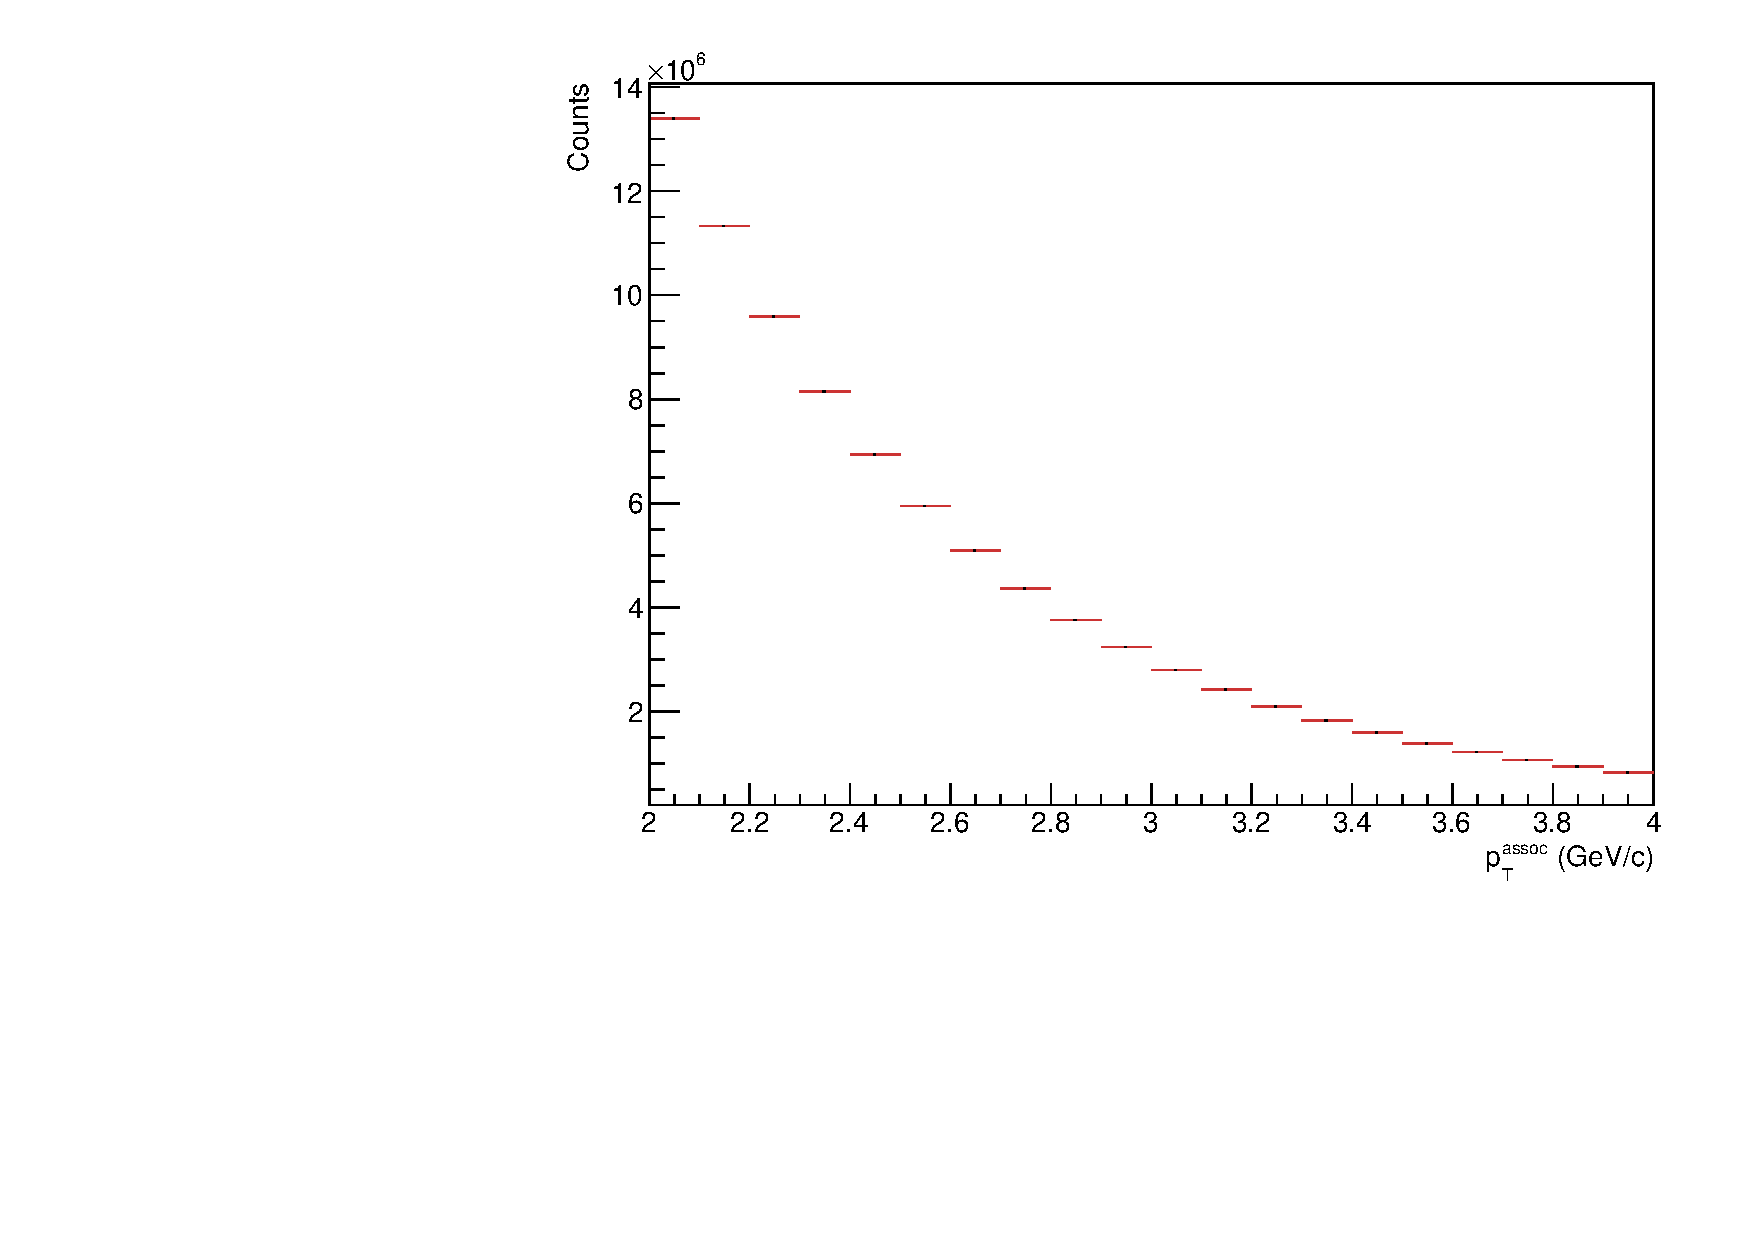
\includegraphics[width=2in]{figures/assoc_pt_dist_0_20.pdf}}
\end{subfigure}
\begin{subfigure}{
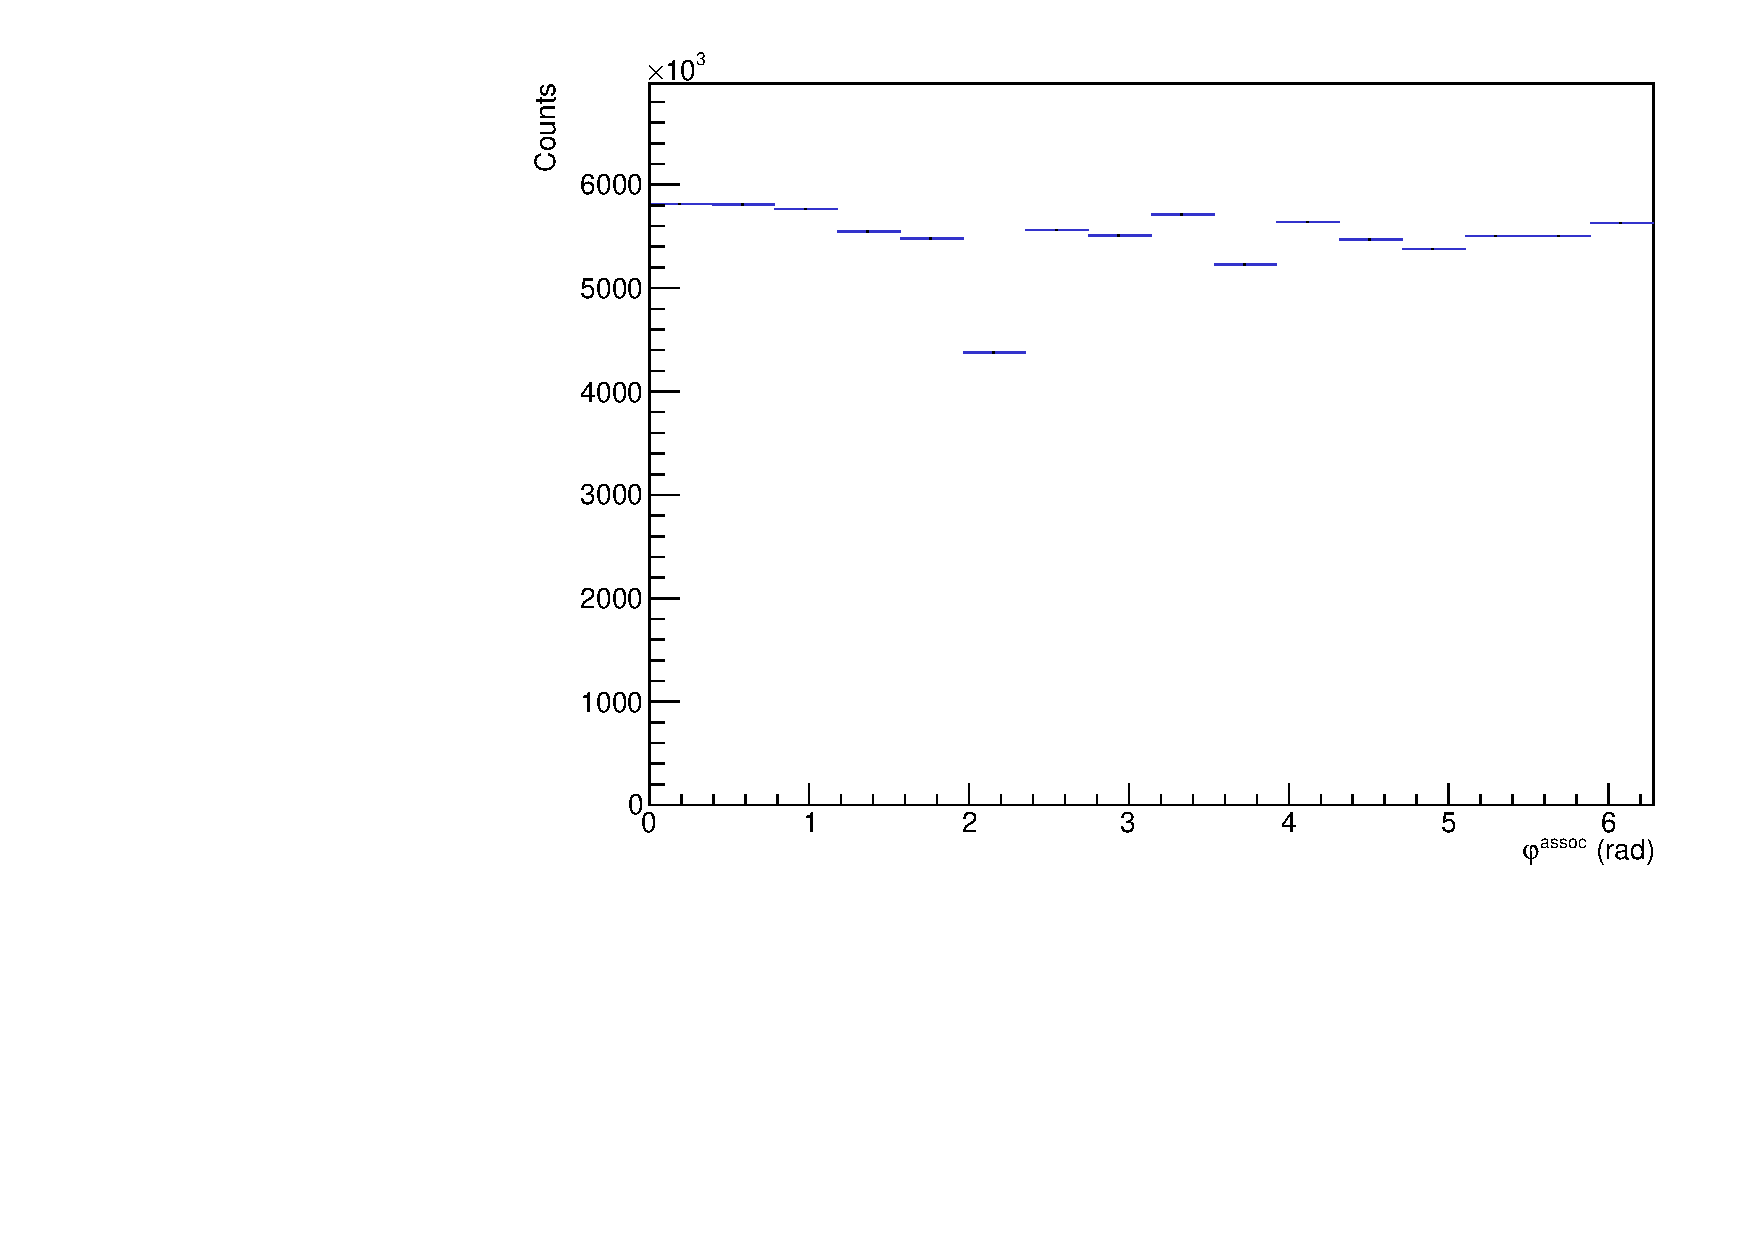
\includegraphics[width=2in]{figures/assoc_phi_dist_0_20.pdf}}
\end{subfigure}
\begin{subfigure}{
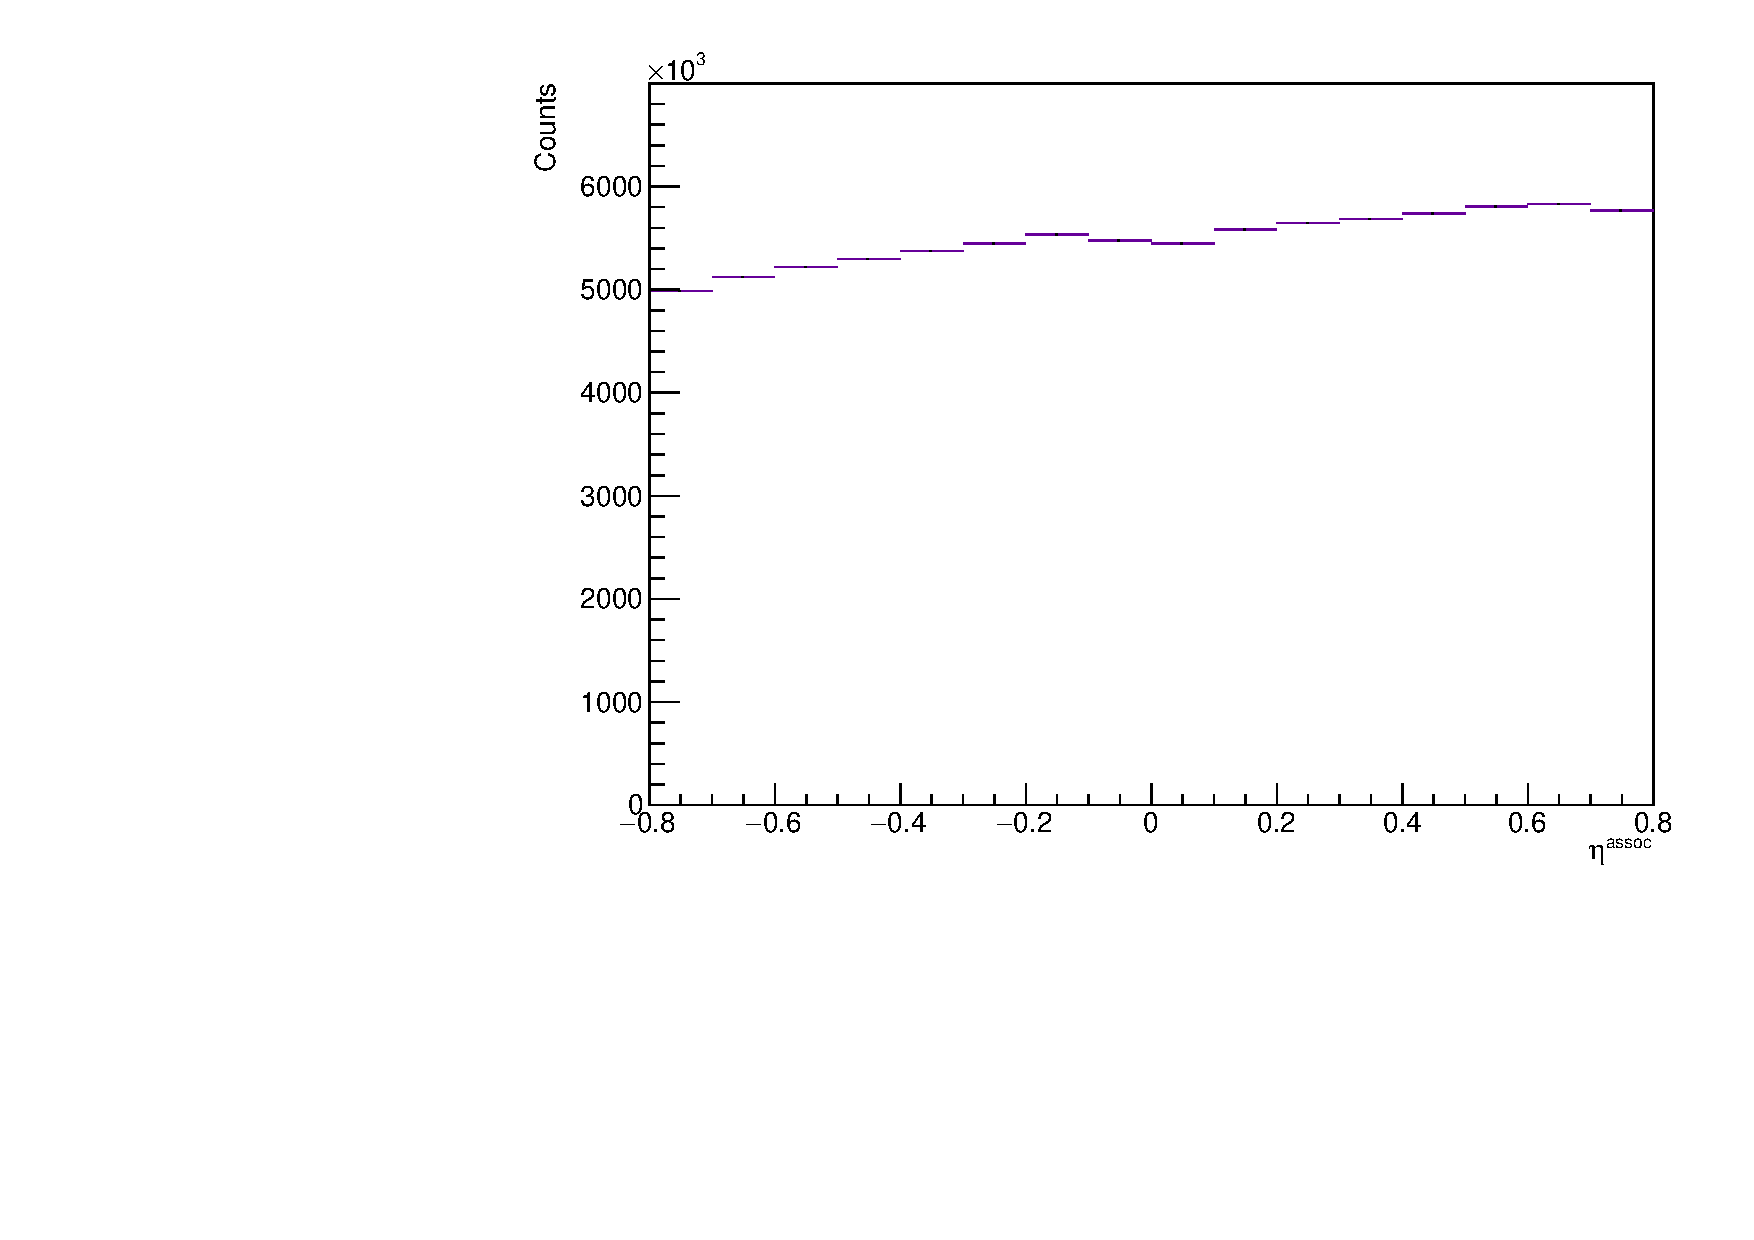
\includegraphics[width=2in]{figures/assoc_eta_dist_0_20.pdf}}
\end{subfigure}
\caption{The $\it{p}_{T}$ (left), $\varphi$ (center) and $\eta$ (right) distributions for the associated hadrons in the multiplicity range 0-20\%.}
\label{assoc_plots}
\end{figure}



\subsection{$\Lambda$ Daughter Proton and Pion Track Cuts}
\label{daughtercuts}
The proton and the pion are required to have a minimum $p_{T}$ of $p_{T} >$ \SI{0.15}{GeV/c} and an $\eta$ cut of $|{\eta}| < 0.8$. Furthermore, the proton and pion are required to meet the following quality cuts:
\begin{itemize}
	\item TPC refit flag enabled
	\item TPC crossed rows $>$ 70
	\item (TPC crossed rows)/(findable clusters) $>$ 0.8
\end{itemize}
All of these cuts are applied to the daughters of the reconstructed $\Lambda$, independent of the technique used for said reconstruction. For the correlation, the reconstructed $\Lambda$ is selected only in the momentum region

$${1.0 < p_{T} < \SI{4.0}{GeV/c}},$$

with further binning performed offline.

\subsubsection{Trigger Track Cuts}
\label{trigcuts}
For the trigger hadron tracks, Hybrid Global constrained tracks were accepted using the cuts supplied by \texttt{IsHybridGlobalConstrainedGlobal()}, or track bit 768:

\begin{itemize}
	\item SetMinNClustersTPC: 50
	\item SetMaxChi2PerClusterTPC: 4
	\item SetAcceptKinkDaughters: kFALSE
	\item SetMaxDCAToVertexZ: 3.2
	\item SetMaxDCAToVertexXY: 2.4
	\item SetDCAToVertex2D: kTRUE
	\item SetMaxChi2TPCConstrainedGlobal(36)
	\item SetMaxFractionSharedTPCClusters(0.4)
\end{itemize}

For the both the di-hadron and h-$\Lambda$ correlation, the trigger hadron is selected in the momentum region:

$${4.0 < p_{T} < \SI{8.0}{GeV/c}},$$

with further binning performed offline. The $\it{p}_{T}$, $\varphi$ and $\eta$ distributions for the trigger hadrons that pass these cuts in the 0-20\% multiplicity bin can be seen in Figure \ref{trig_plots}.

\begin{figure}[ht]
\centering
\begin{subfigure}{
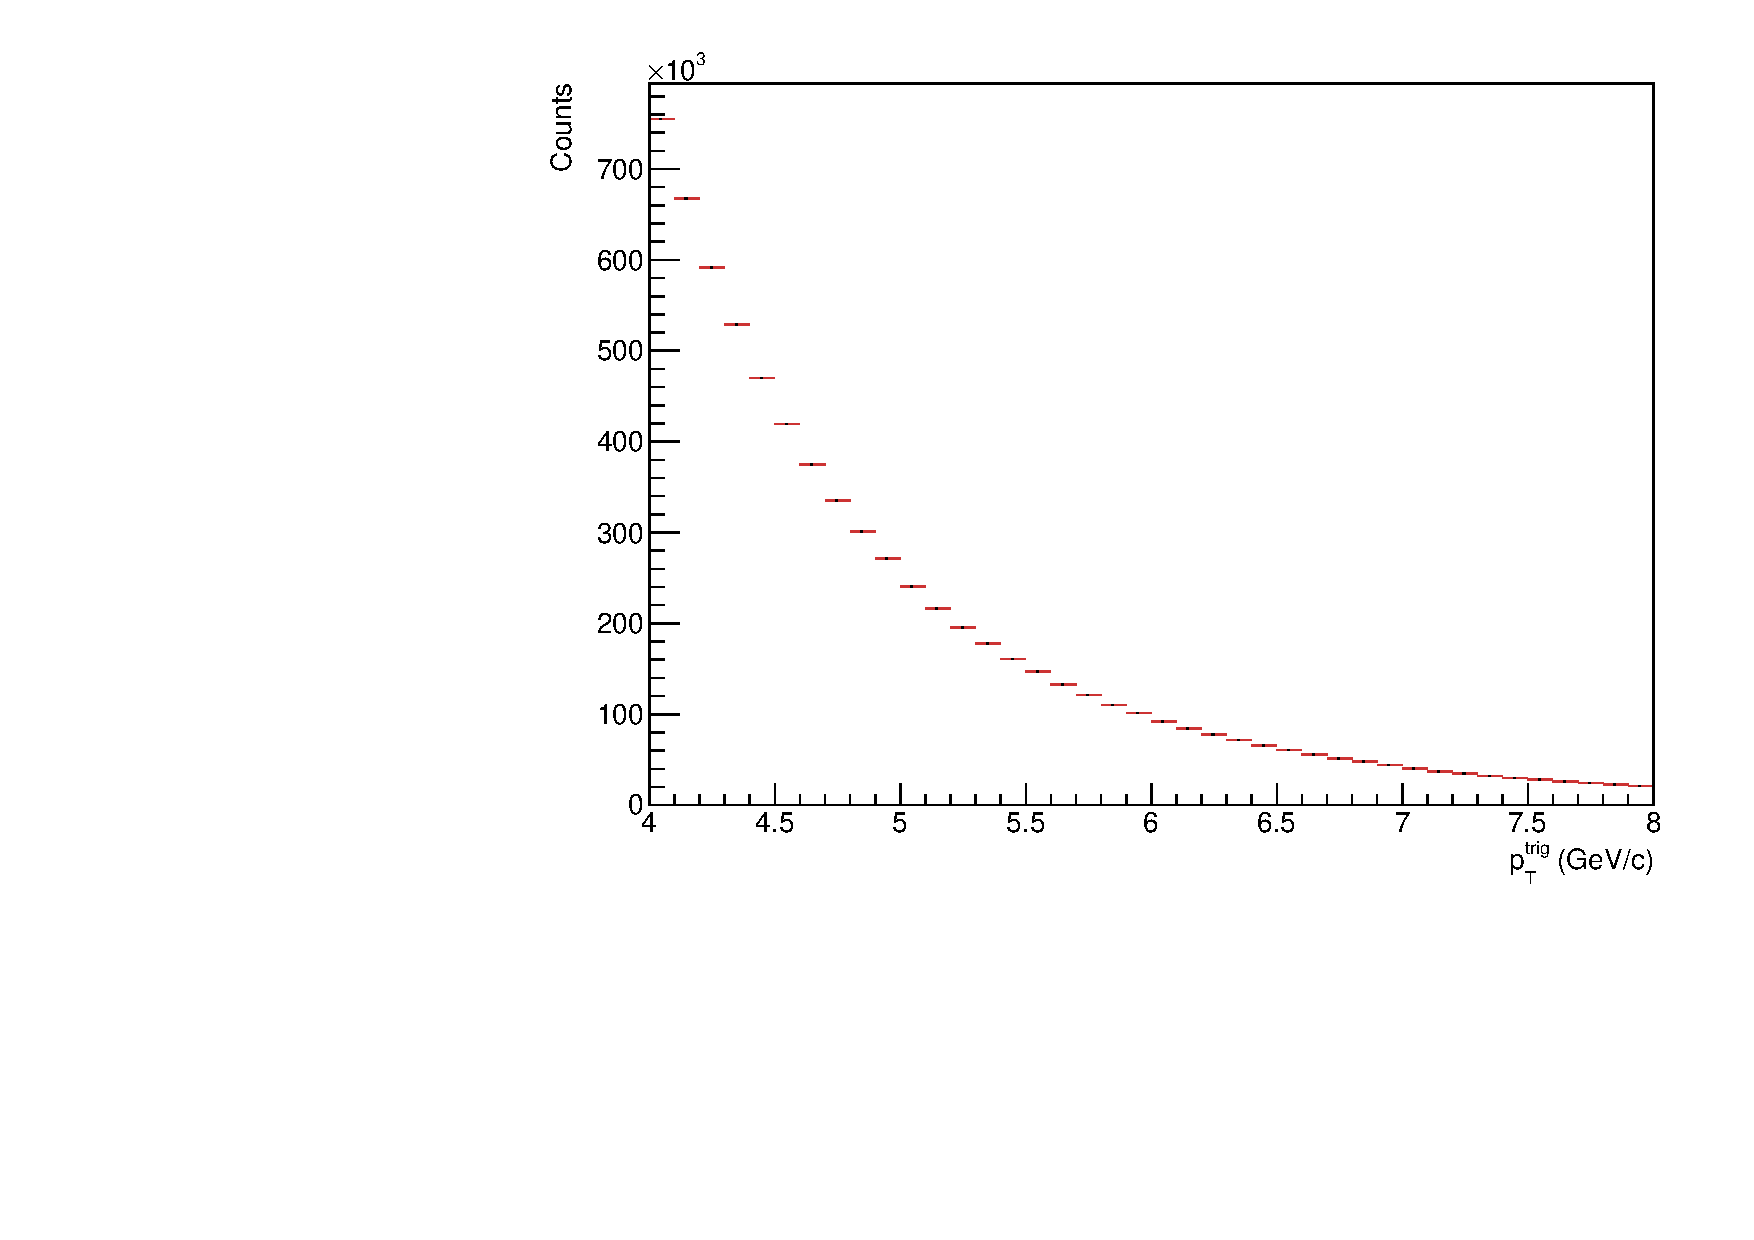
\includegraphics[width=2in]{figures/trig_pt_dist_0_20.pdf}}
\end{subfigure}
\begin{subfigure}{
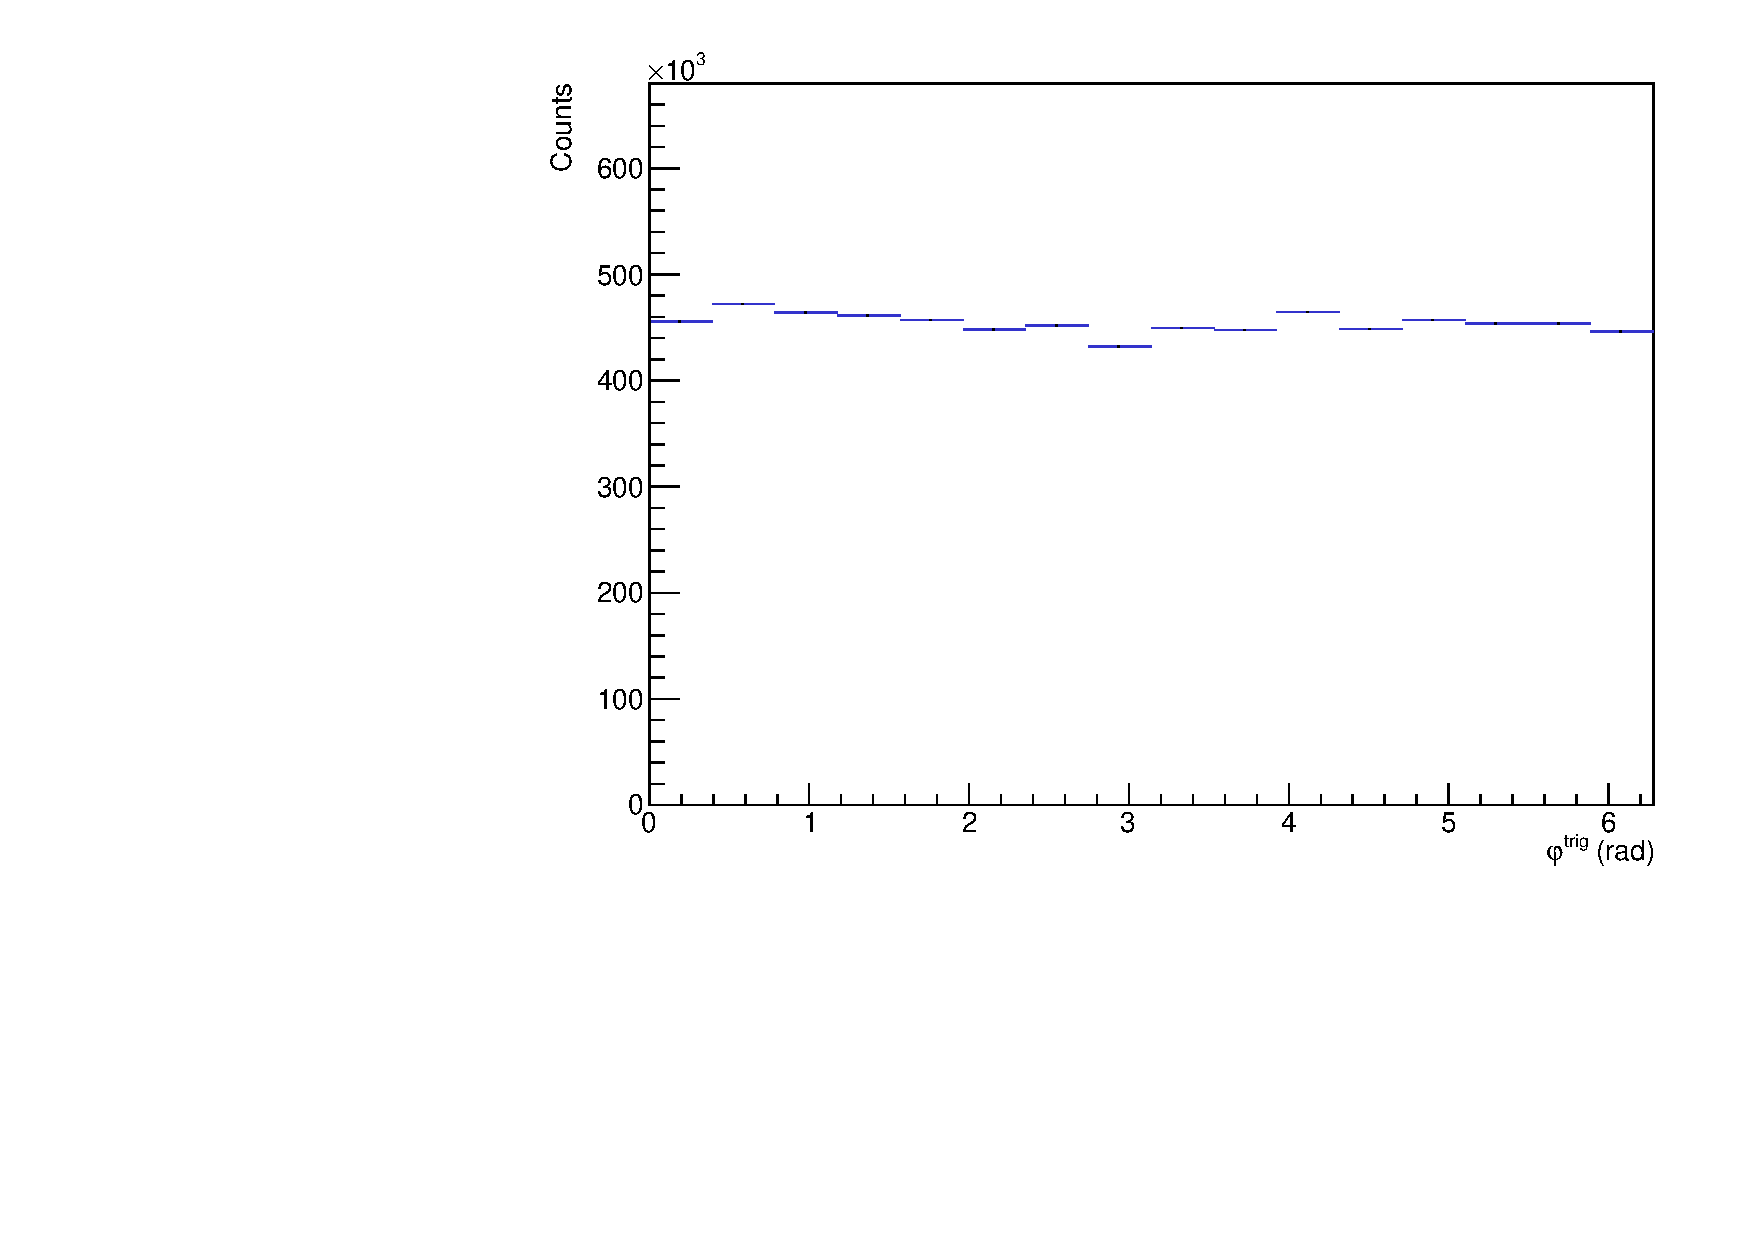
\includegraphics[width=2in]{figures/trig_phi_dist_0_20.pdf}}
\end{subfigure}
\begin{subfigure}{
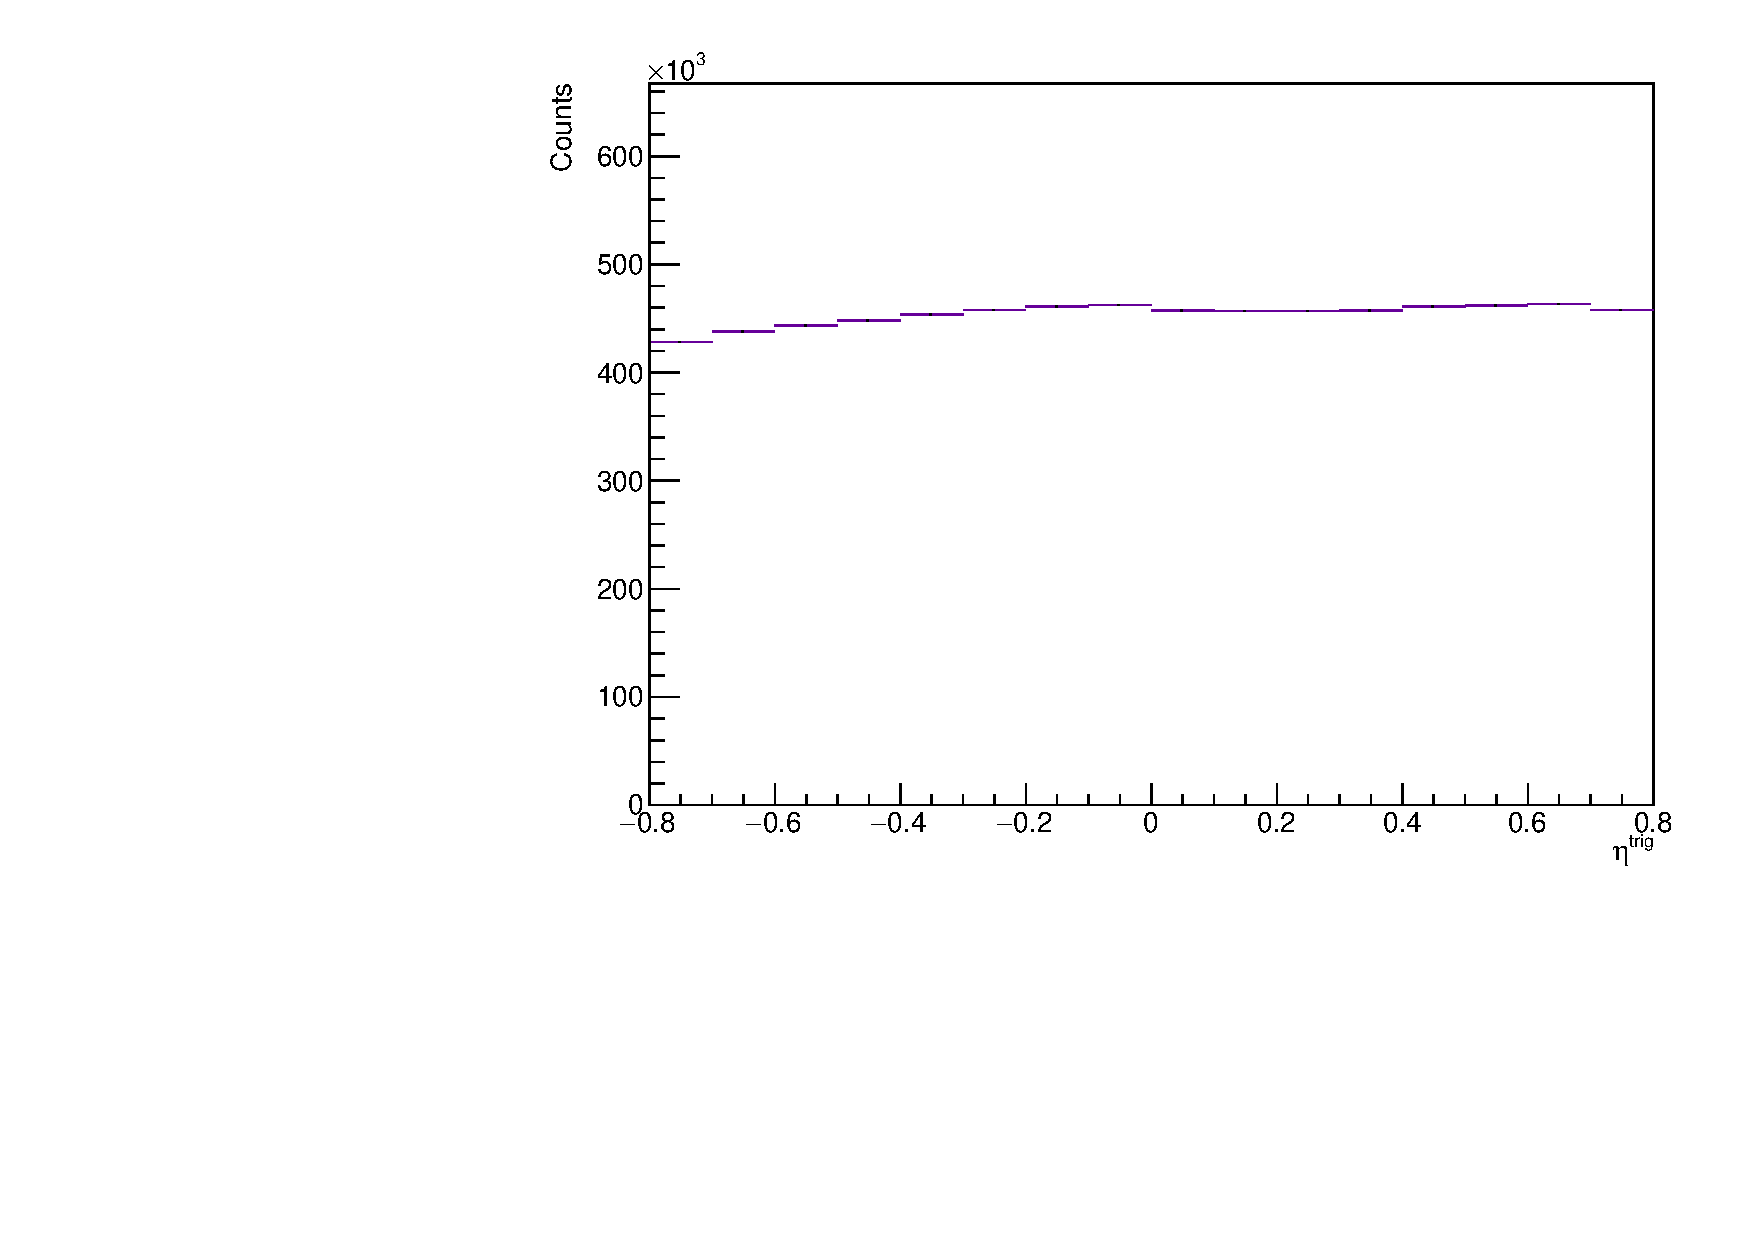
\includegraphics[width=2in]{figures/trig_eta_dist_0_20.pdf}}
\end{subfigure}
\caption{The $\it{p}_{T}$ (left), $\varphi$ (center) and $\eta$ (right) distributions for the trigger hadrons in the multiplicity range 0-20\%. Note that the $\varphi$ and $\eta$ distributions are uniform, indicating no geometric biases from track selection (TPC sector bounds, etc.) will be introduced into the angular correlations.}
\label{trig_plots}
\end{figure}

\section{$\Lambda$ Reconstruction}
\label{lambda_reconstruction}

The $\Lambda$ candidates were reconstructed through the $\Lambda \rightarrow p\pi^{-}$ ($\bar{\Lambda} \rightarrow \pi^{+}p$) decay channel with a branching ratio of 63.9\%. For the majority of this analysis, the $\Lambda$ and $\bar{\Lambda}$ are combined together. Thus, unless otherwise specified, $\Lambda = \Lambda + \bar{\Lambda}$. 

The $\Lambda$ candidates in this analysis were reconstructed using two separate techniques:
\begin{itemize}
	\item \textbf{V0 Finder Technique} - The V0 finder technique reconstructs the $\Lambda$ by combining the proton and pion tracks with the V0 finder algorithm, which can be found within the AliROOT framework.
	\item \textbf{Resonance Technique} - The resonance technique combines all oppositely charged proton-pion pairs to reconstruct the $\Lambda$, resulting in maximal statistics at the cost of a large combinatorial background.
\end{itemize}

The central points in this analysis are from $\Lambda$ candidates reconstructed using the V0 finder technique. The resonance technique serves as a powerful cross-check to ensure no topological biases are introduced within the V0 finder algorithm, and is investigated in detail in Section \ref{resonance_technique}.

\subsection{V0 Selection}
\label{v0_selection}
The central points in this analysis were generated using $\Lambda$s reconstructed using the V0-finder algorithm found within the AliROOT framework. All of the V0s found by the V0 finder algorithm were required to pass the following cuts:

\begin{itemize}
	\item $p_{T} > 0.2$ GeV/$c$
	\item $|\eta| < 0.8$
	\item On the fly status: disabled (offline V0s only)
\end{itemize}

There were no additional topological cuts applied to the V0s or their corresponding daughters. This was done to maximize statistics and to minimize any topological biases introduced by reconstructing $\Lambda$s using the V0-finder algorithm itself. 

\subsection{V0 Daughter PID Cuts}
\label{v0_daughter_pid}
The daughter protons and pions were required to meet the following PID cuts using both the TPC and TOF detectors:

\begin{itemize}
	\item[$\ast$] $|n\sigma_{TPC, p}| < 2$
	\item[$\ast$] $|n\sigma_{TPC, \pi}| < 3$
	\item[$\ast$] $|n\sigma_{TOF, p}| < 2$ (if signal exists)
	\item[$\ast$] $|n\sigma_{TOF, \pi}| < 3$ (if signal exists)
\end{itemize}


\begin{figure}[ht]
\centering
\begin{subfigure}{
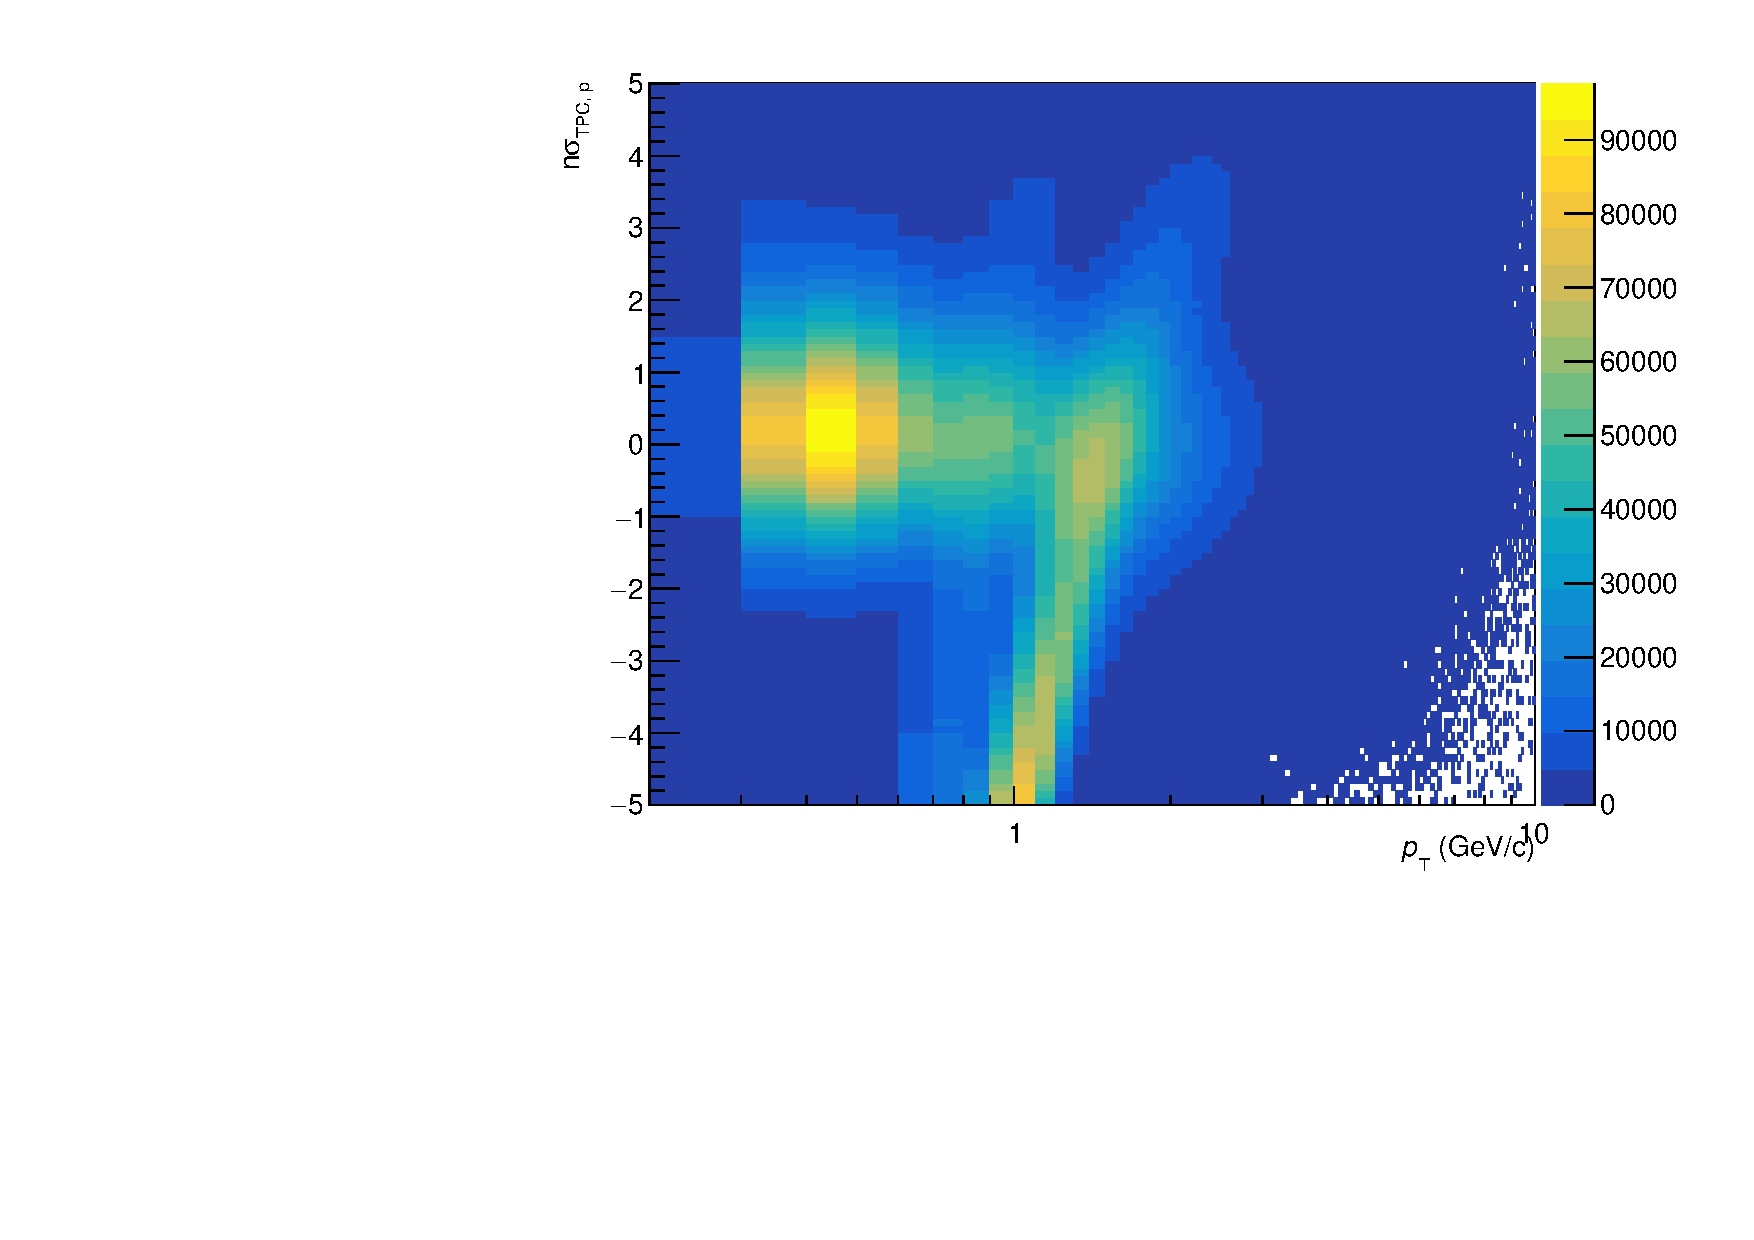
\includegraphics[width=3in]{figures/nsigma_tpc_proton.pdf}}
\end{subfigure}
\begin{subfigure}{
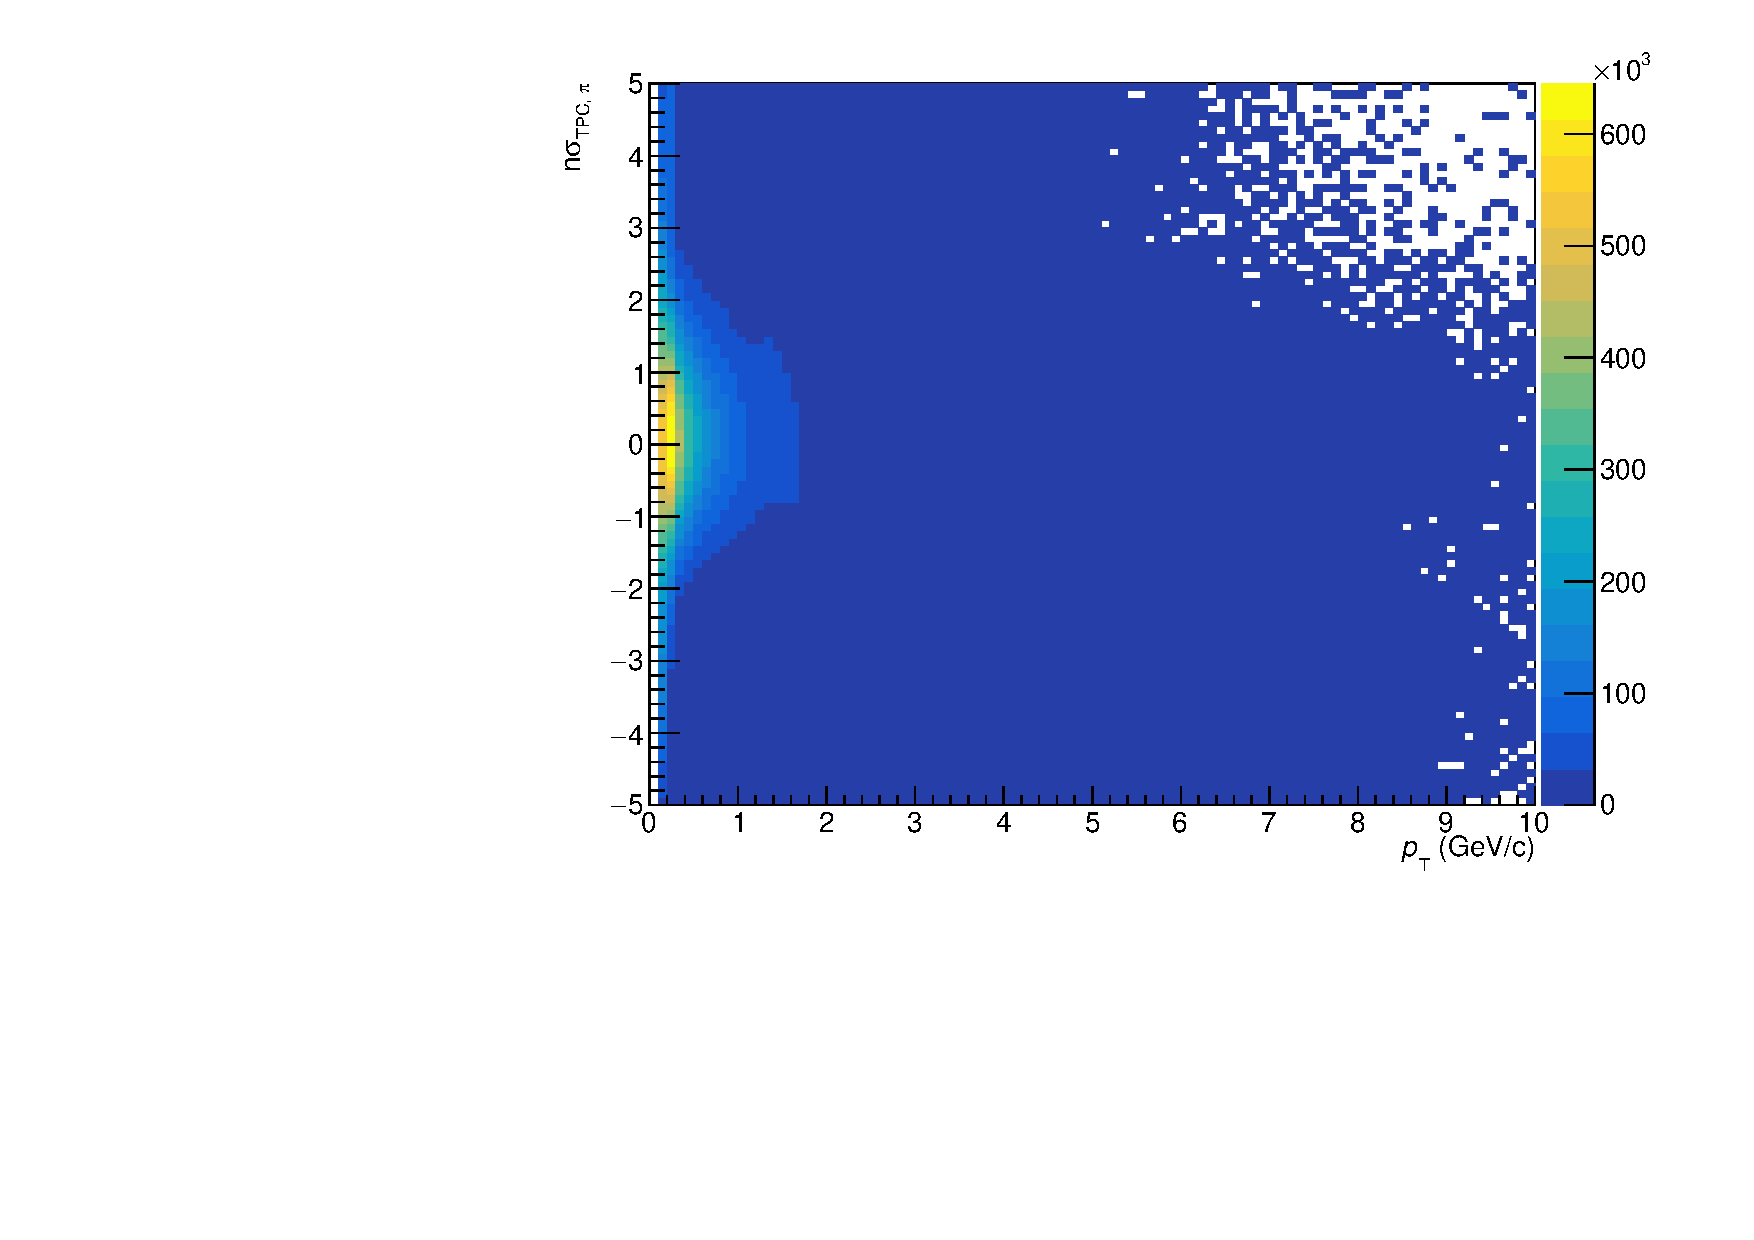
\includegraphics[width=3in]{figures/nsigma_tpc_pion.pdf}}
\end{subfigure}
\caption{$n\sigma$ for protons (left) and pions (right) in the TPC detector as a function of $p_{T}$. A wider PID cut is used for the pion to maximize the $\Lambda$ signal.}
\label{nsigma_tpc}
\end{figure}

\begin{figure}[ht]
\centering
\begin{subfigure}{
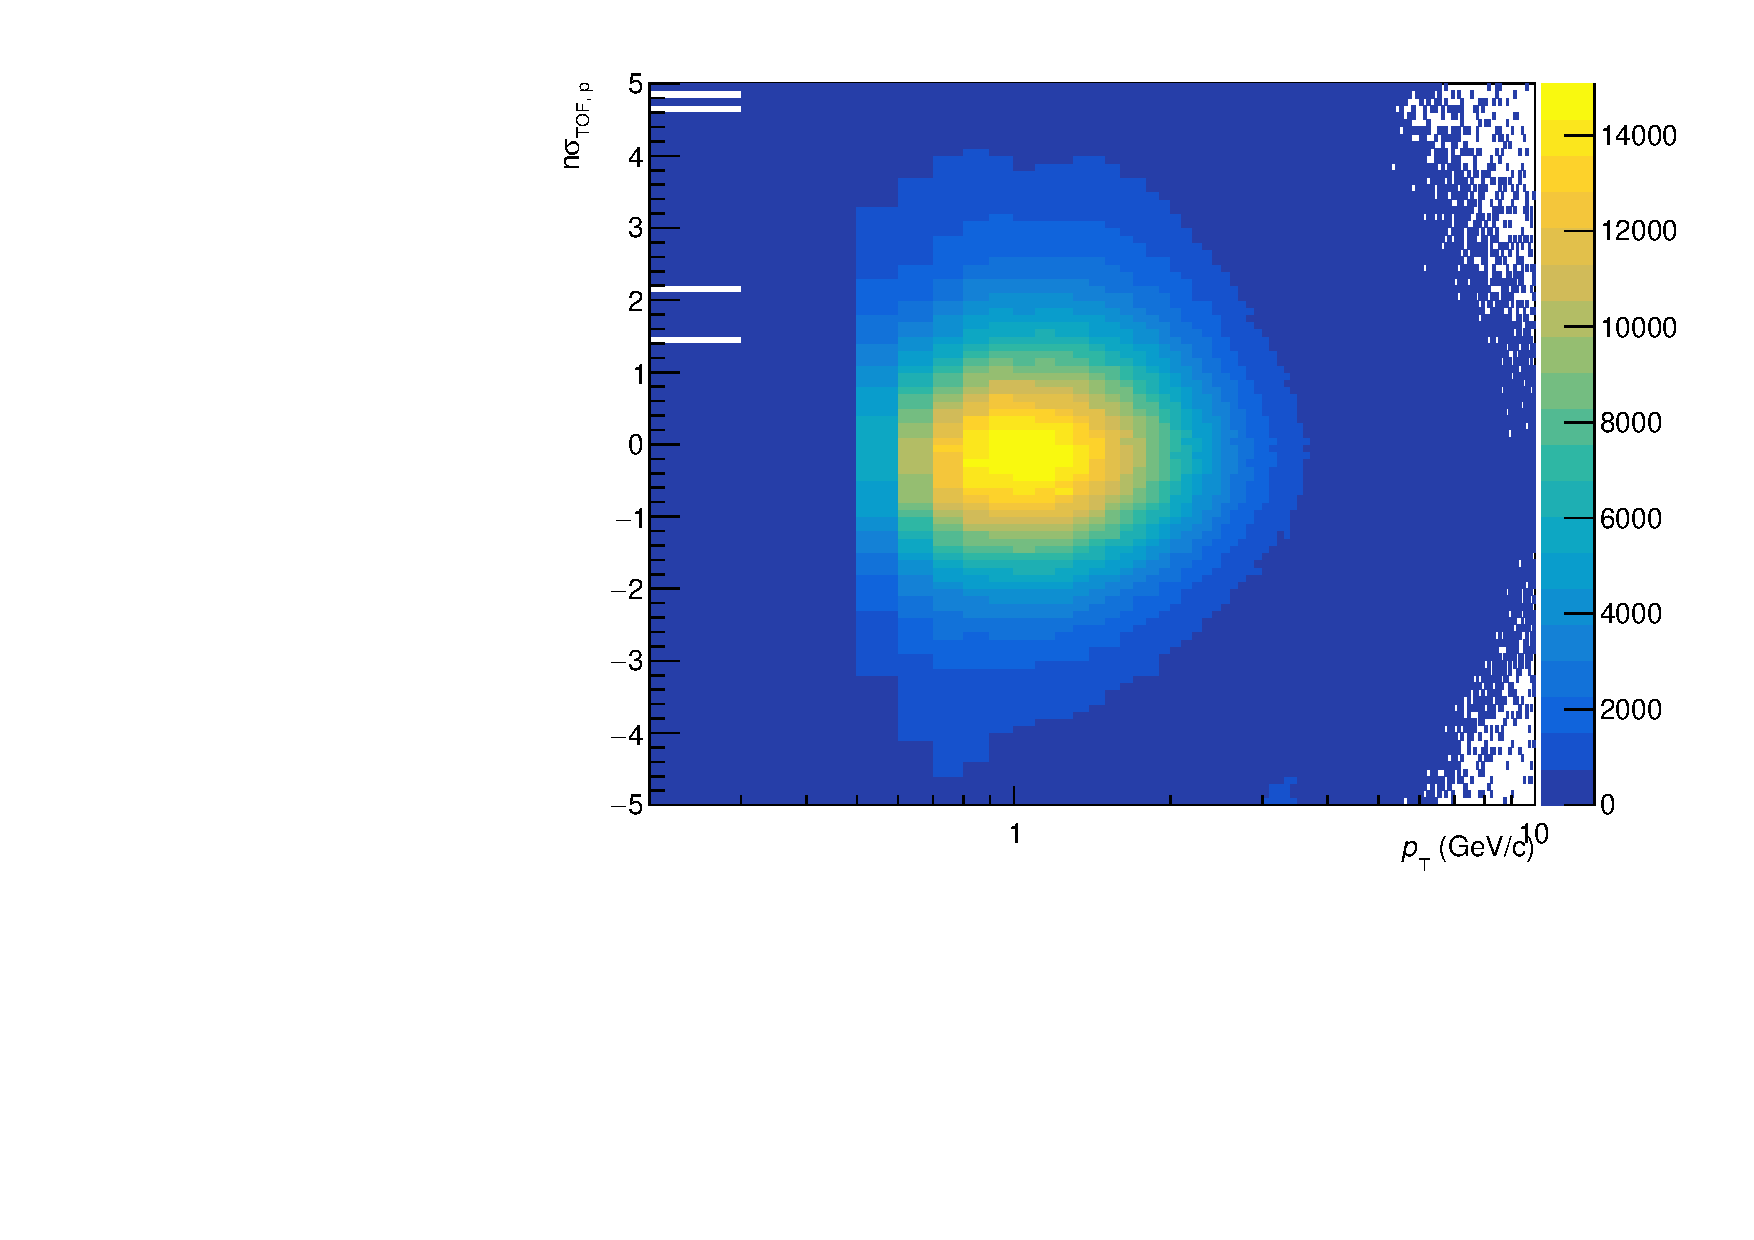
\includegraphics[width=3in]{figures/nsigma_tof_proton.pdf}}
\end{subfigure}
\begin{subfigure}{
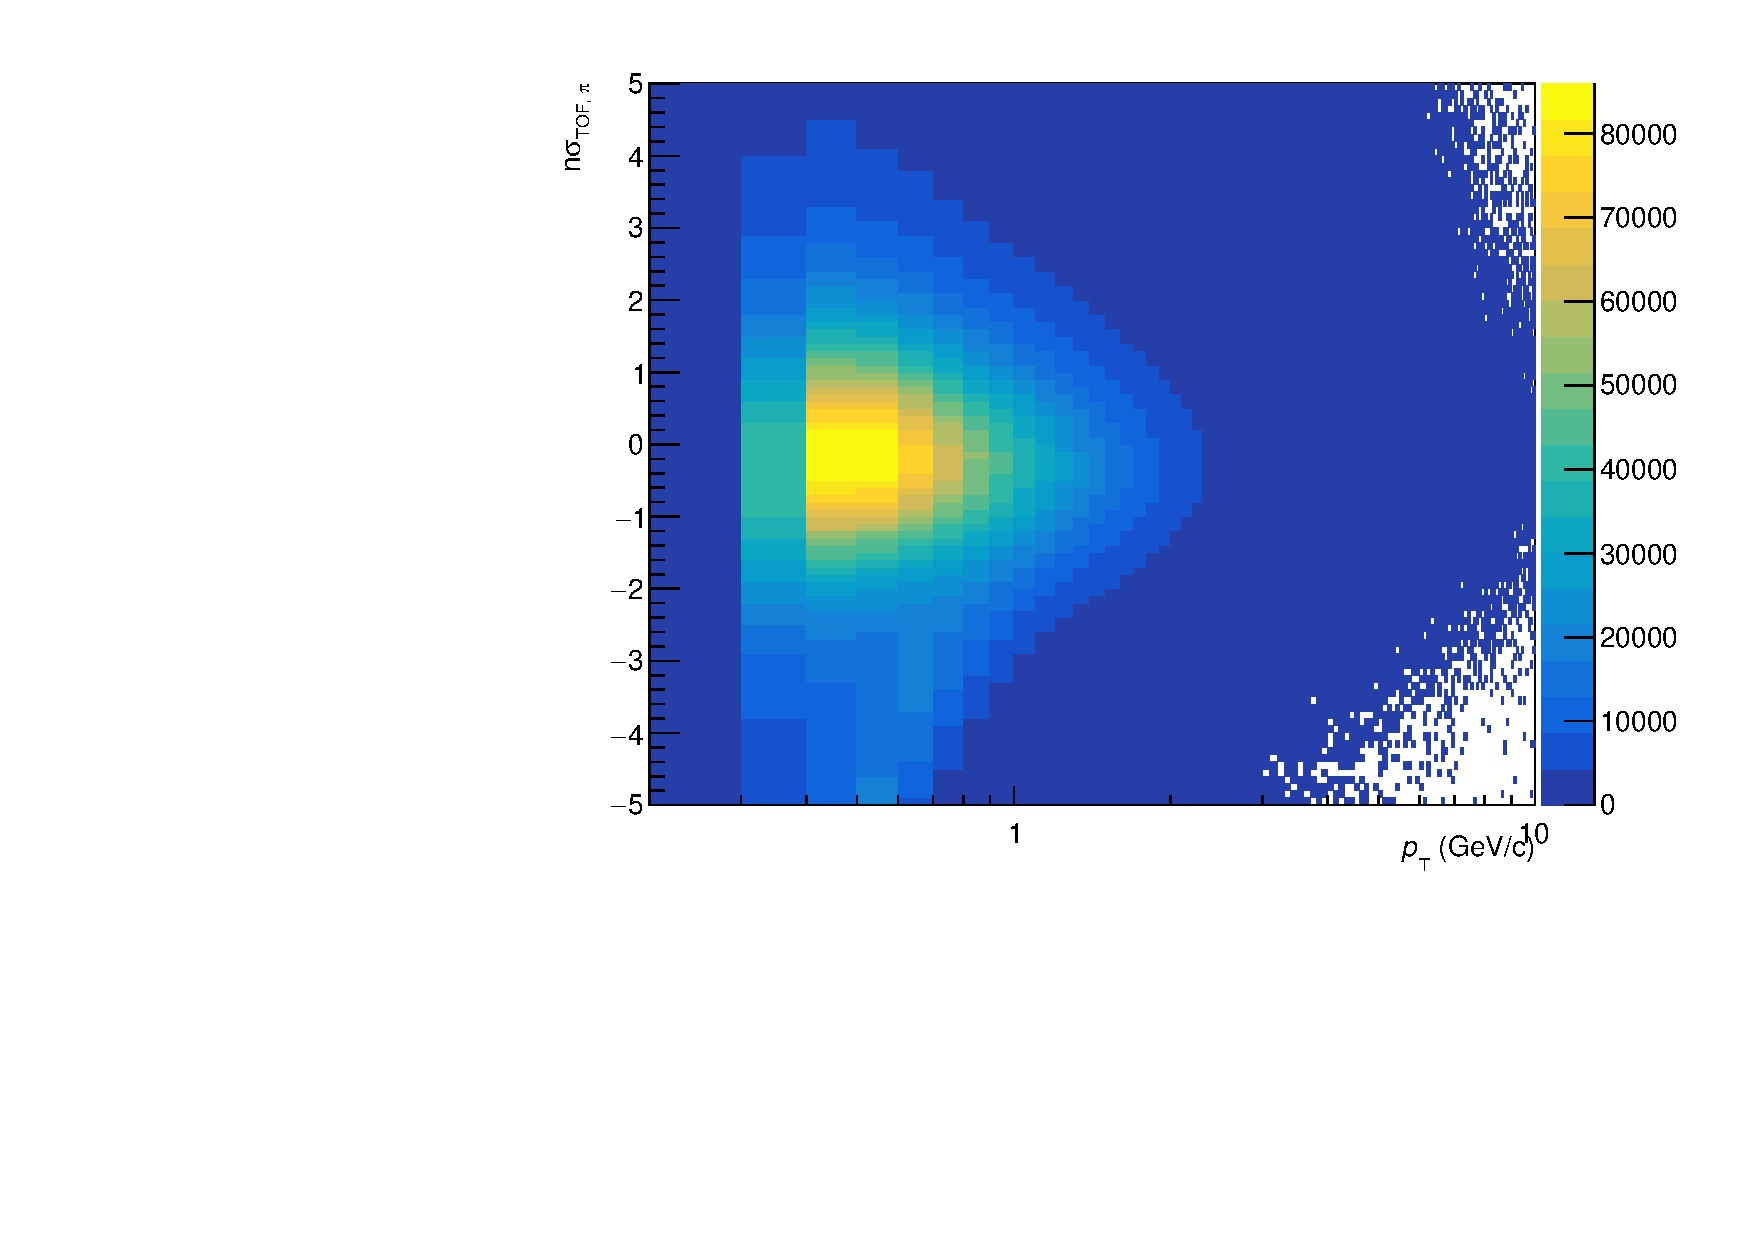
\includegraphics[width=3in]{figures/nsigma_tof_pion.pdf}}
\end{subfigure}
\caption{$n\sigma$ for pions (left) and pions (right) in the TOF detector as a function of $\it{p}_{T}$. If there is no TOF signal for the track, the TOF PID cut is not applied.}
\label{nsigma_tof}
\end{figure}

The $n\sigma$ values for both the TPC and TOF detectors of the daughter proton and pion are shown in Figure \ref{nsigma_tpc} and Figure \ref{nsigma_tof}, respectively. These values were obtained from the AOD tracks associated with every V0 found by the V0 finder algorithm, provided that those tracks also pass the aforementioned daughter track quality cuts.

\begin{figure}[ht]
\centering
\begin{subfigure}{
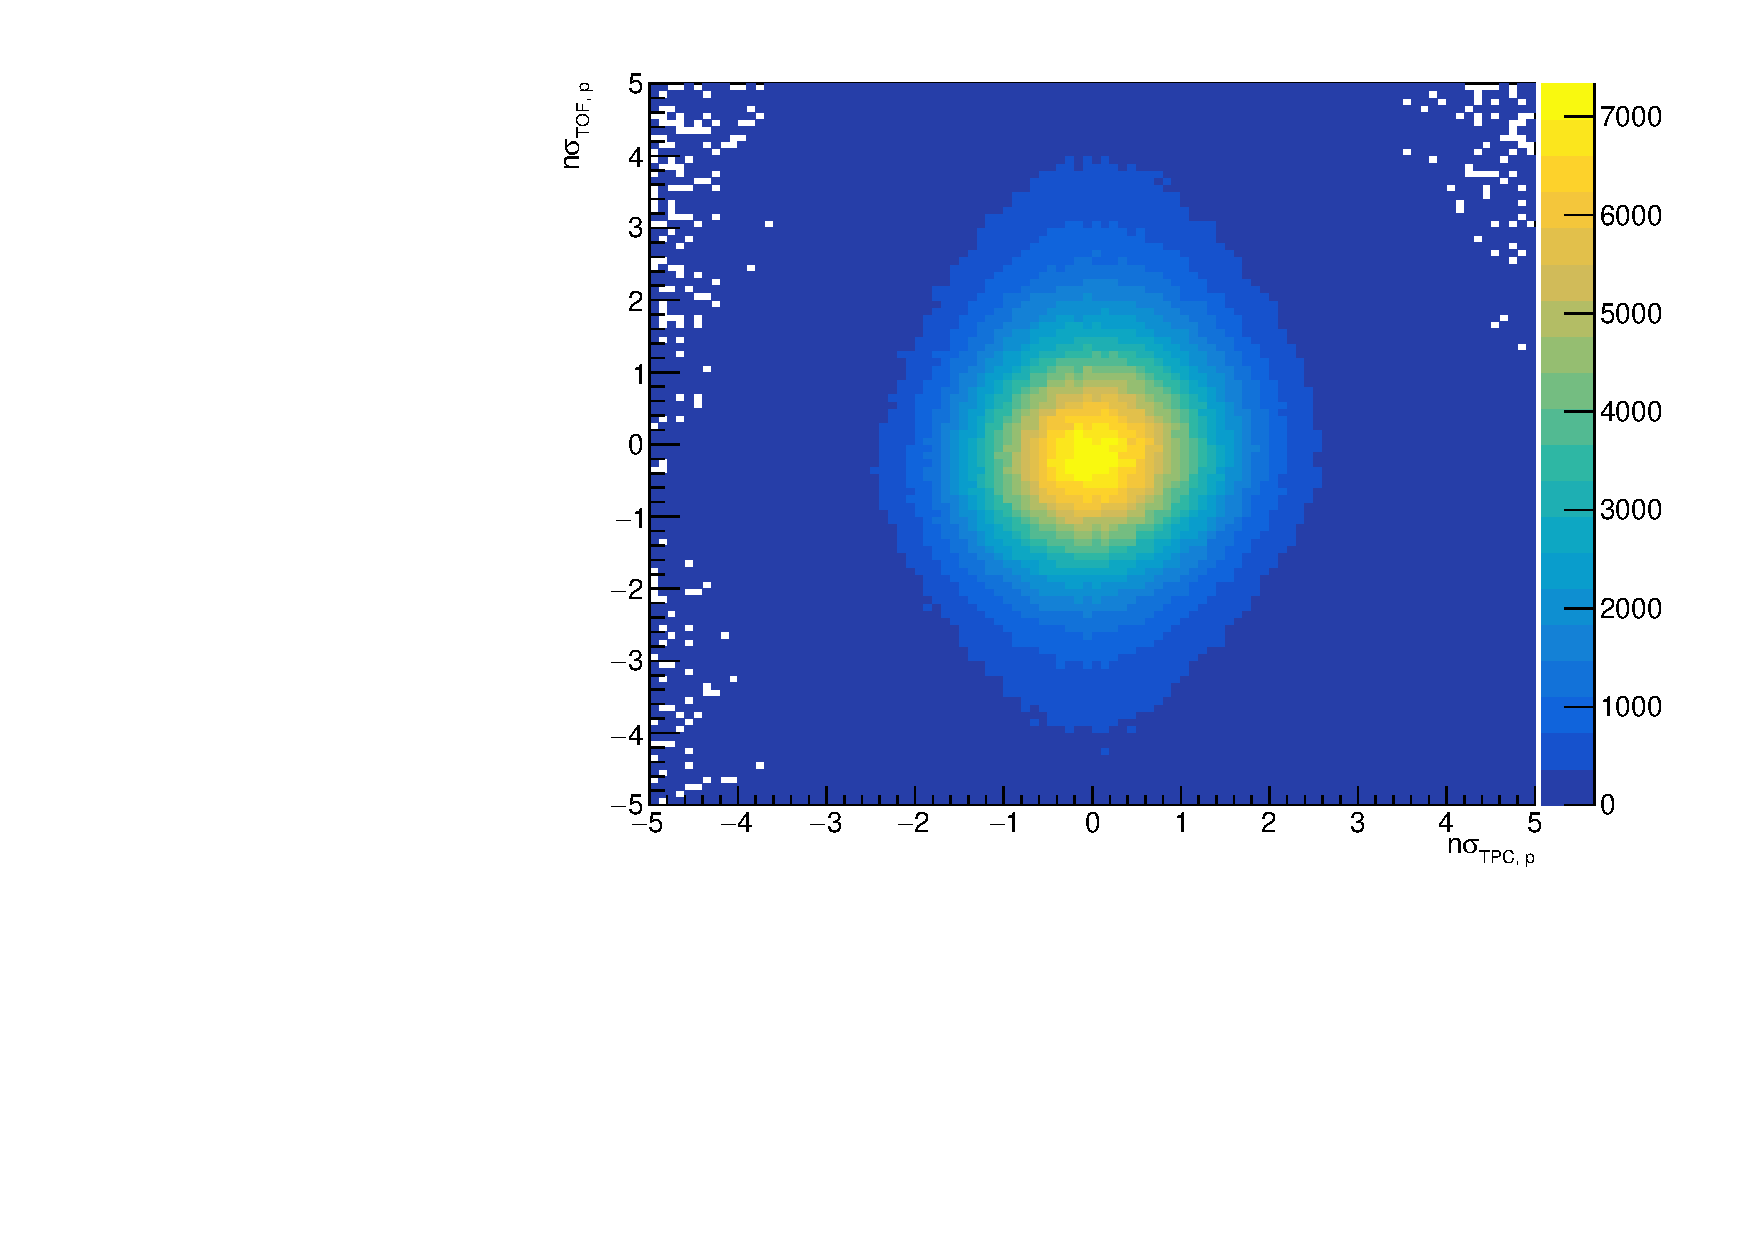
\includegraphics[width=3in]{figures/nsigma_tof_v_tpc_proton.pdf}}
\end{subfigure}
\begin{subfigure}{
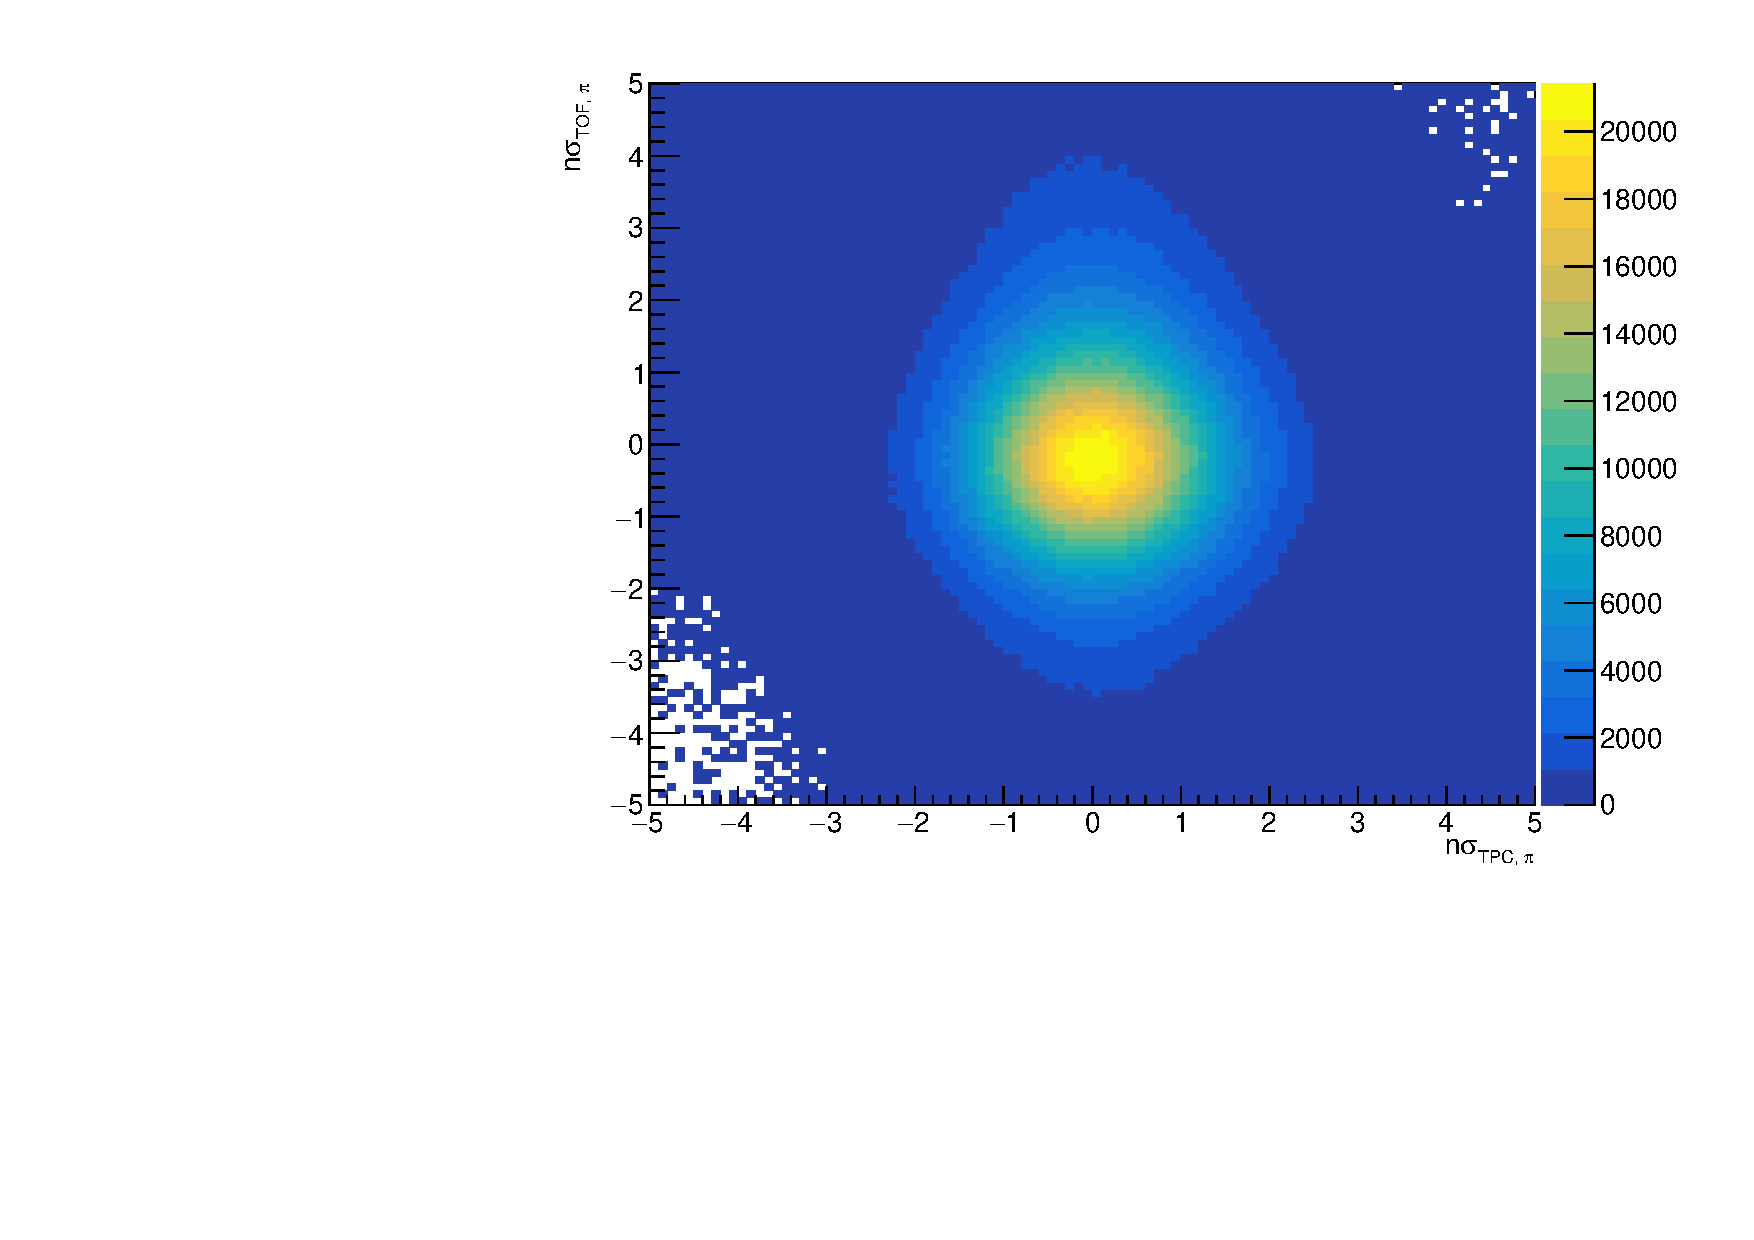
\includegraphics[width=3in]{figures/nsigma_tof_v_tpc_pion.pdf}}
\end{subfigure}
\caption{$n\sigma$ in TOF vs $n\sigma$ in TPC for protons (left) and pions (right). No contimatination is observed for both of the particle species.}
\label{nsigmatofvtpc}
\end{figure}
 
To account for any biases introduced from choosing daughter tracks from the V0 finder algorithm, the TPC and TOF $n\sigma_{p, \pi}$ distributions are shown for all AOD tracks in the tracklist in Figure \ref{nsigmatofvtpc}. There are no major differences between the $n\sigma$ distributions of the daughter tracks from the V0 finder algorithm and the AOD tracks in the tracklist. This indicates that the V0 finder algorithm is not introducing any biases in the PID selection of the daughter tracks. These plots also represent the PID cuts used for the resonance technique, which utilizes the full AOD track list and will be discussed in Section \ref{resonance_technique}.


\begin{figure}[ht]
\centering
\begin{subfigure}{
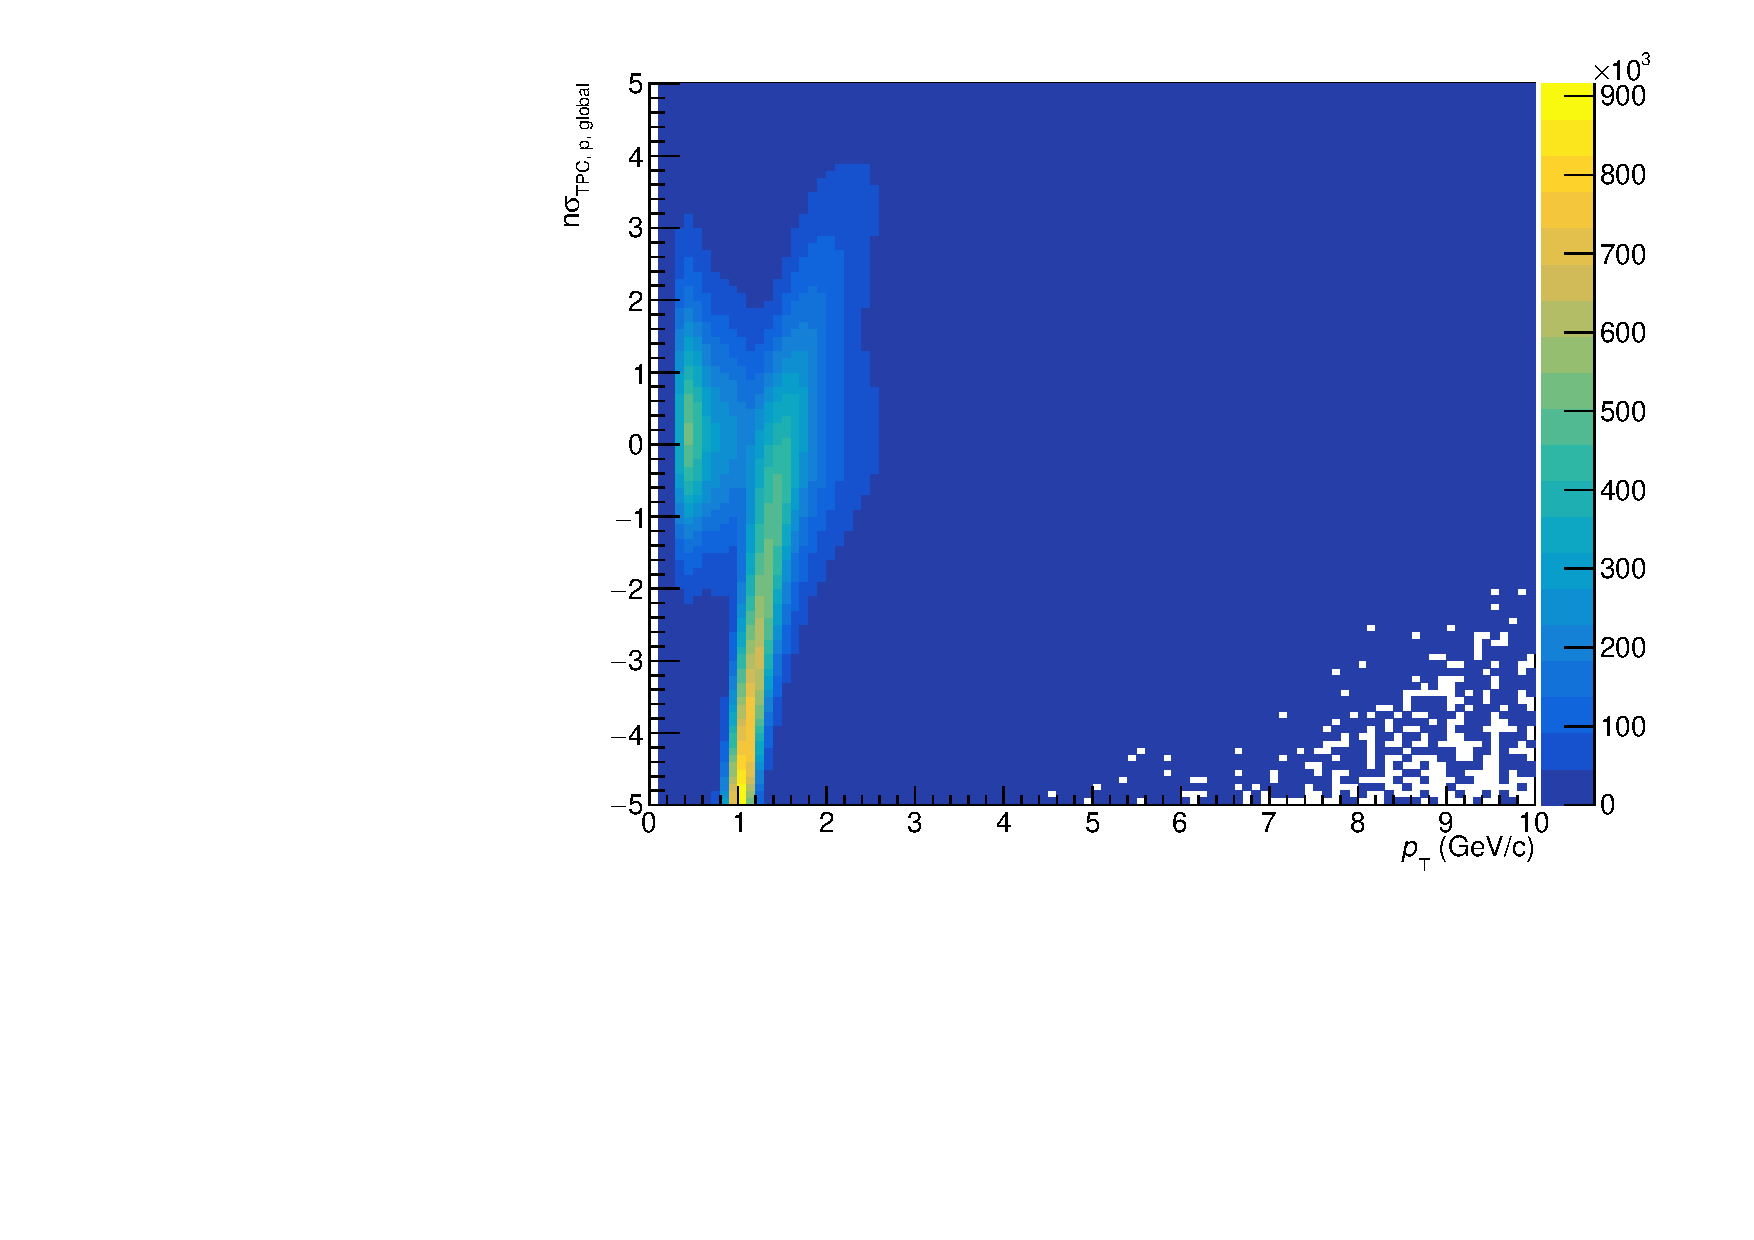
\includegraphics[width=3in]{figures/nsigma_tpc_proton_global.pdf}}
\end{subfigure}
\begin{subfigure}{
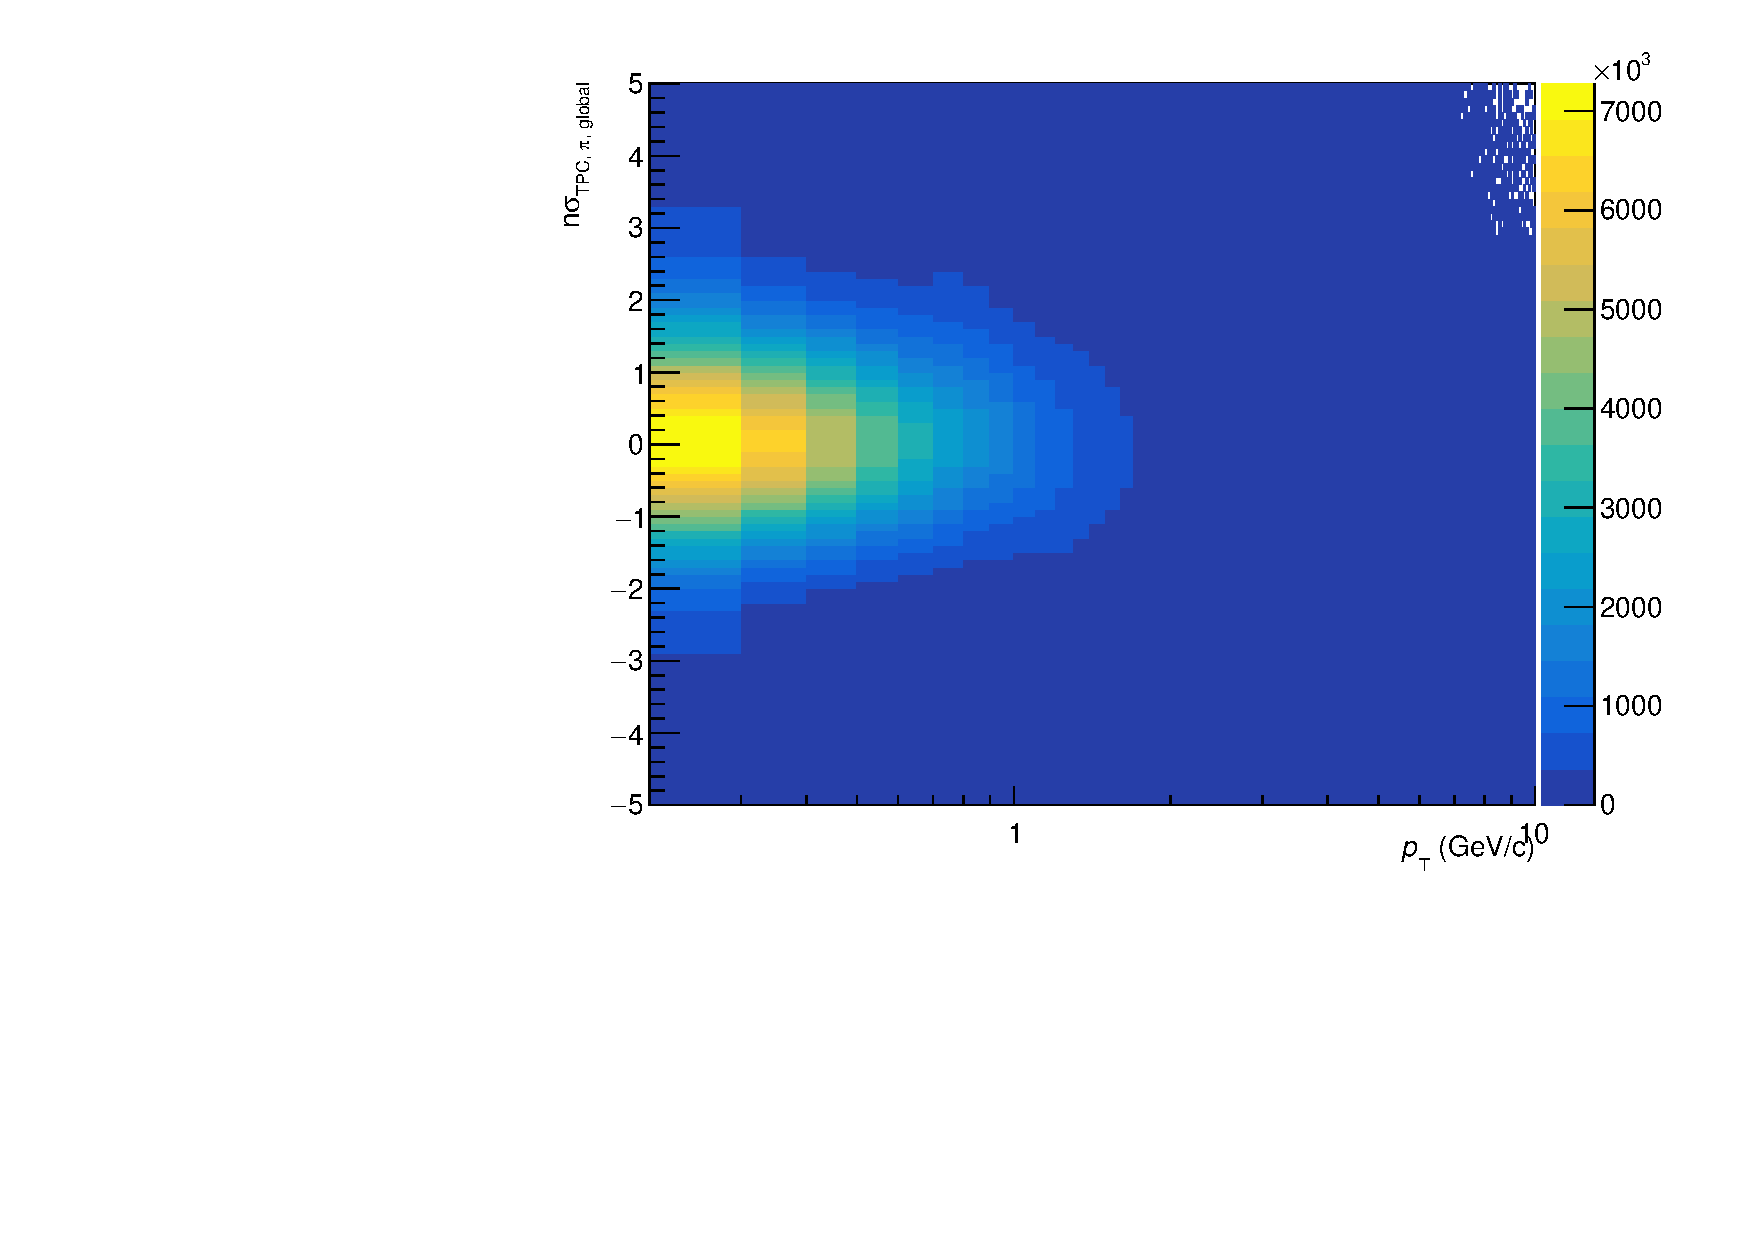
\includegraphics[width=3in]{figures/nsigma_tpc_pion_global.pdf}}
\end{subfigure}
\caption{$n\sigma$ for protons (left) and pions (right) from the global AOD track list in the TPC detector as a function of $p_{T}$. These plots are very similar to those generated from V0 daughter tracks, so we conclude no PID biases are introduced from the V0 finder method.}
\label{nsigma_tpc_global}
\end{figure}

\begin{figure}[ht]
\centering
\begin{subfigure}{
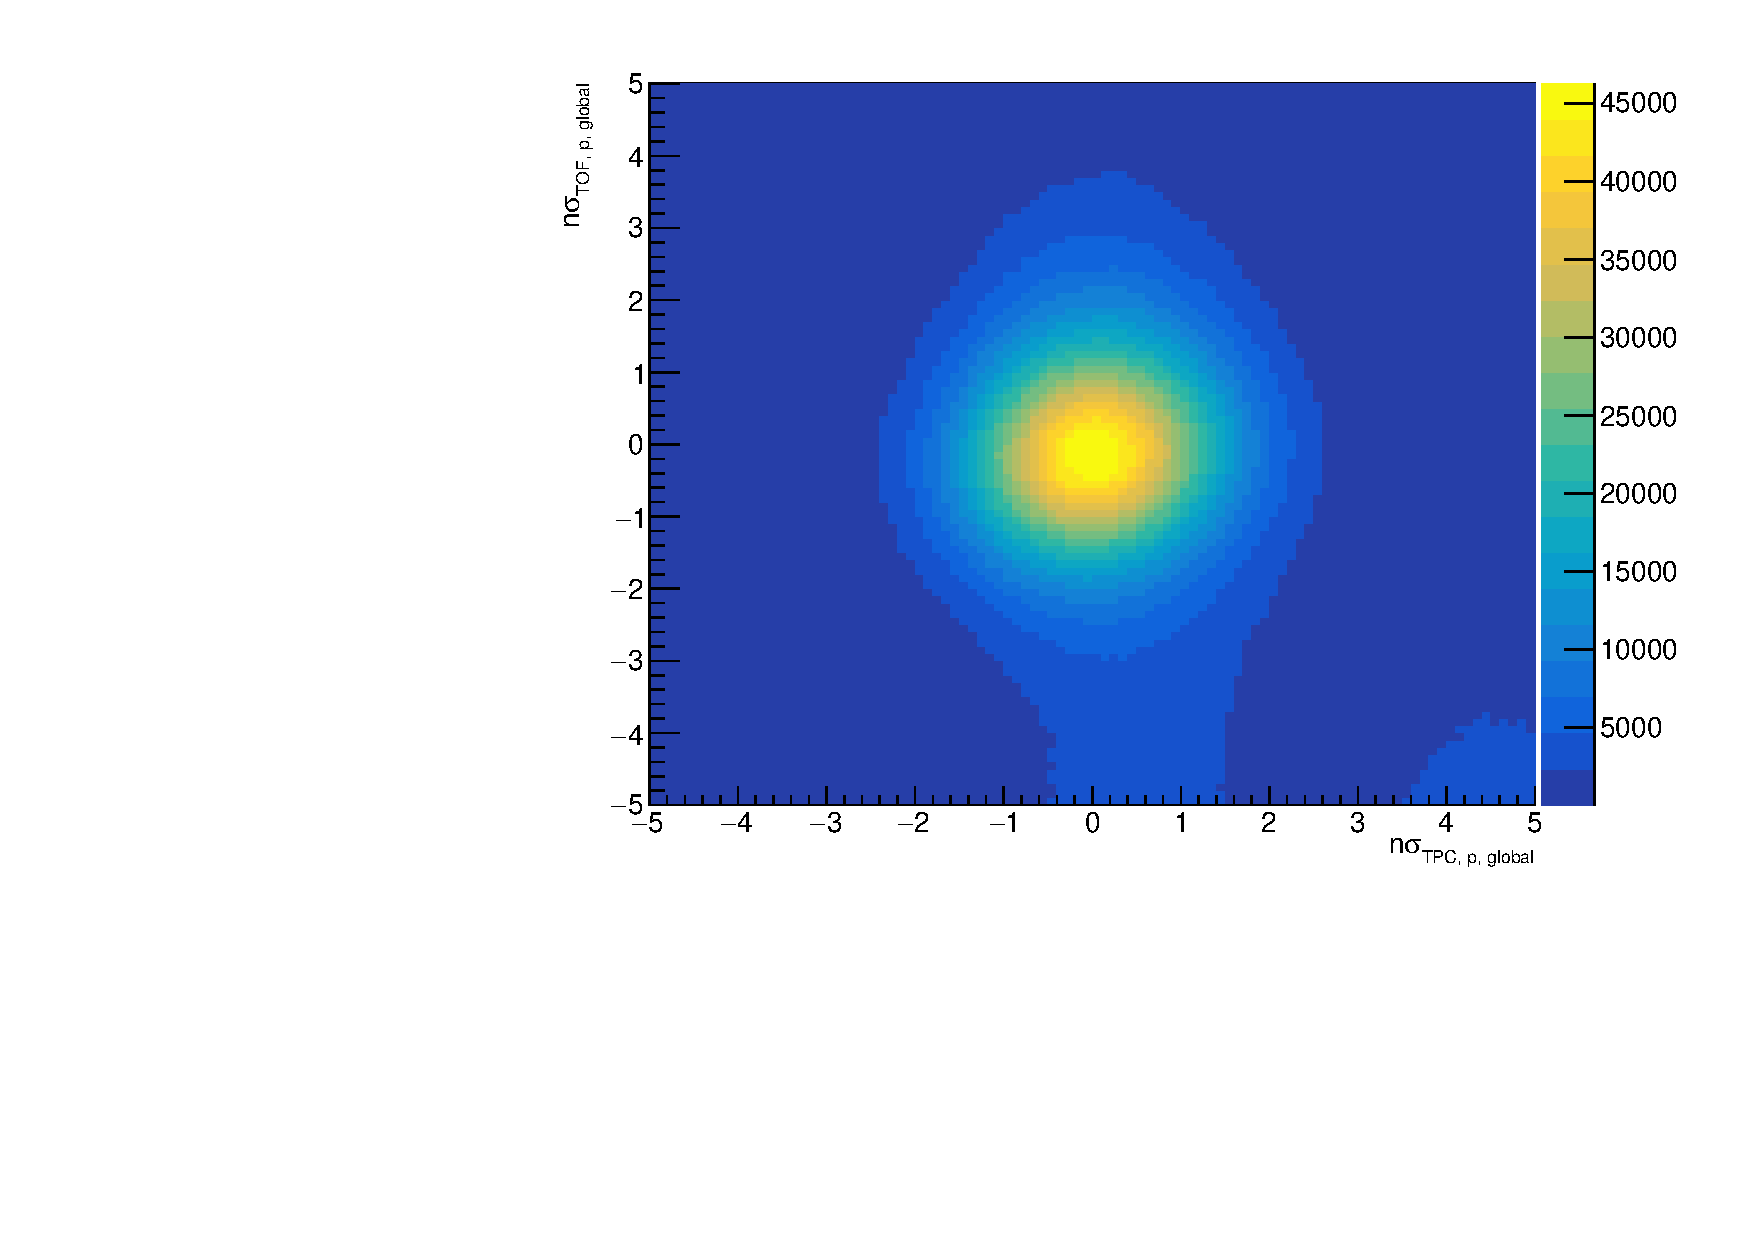
\includegraphics[width=3in]{figures/nsigma_tof_v_tpc_proton_global.pdf}}
\end{subfigure}
\begin{subfigure}{
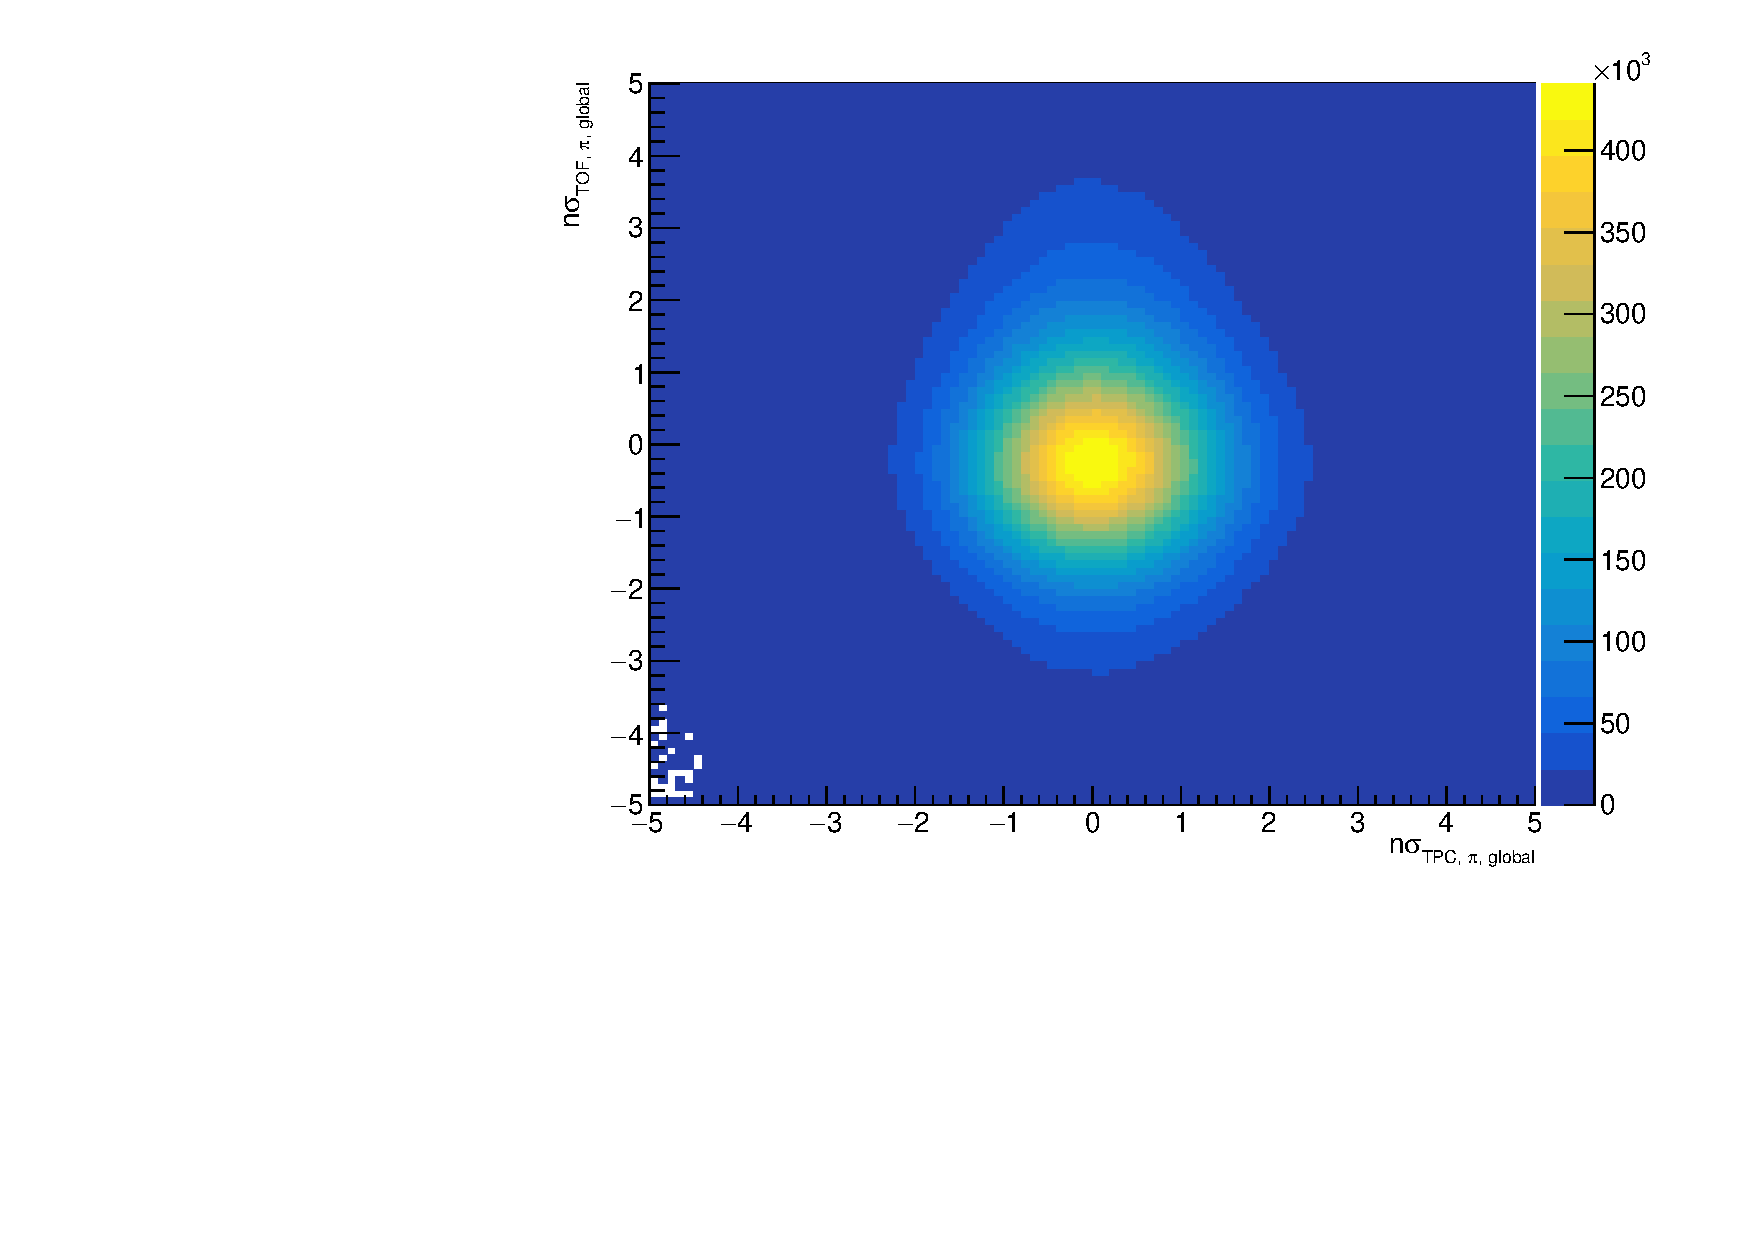
\includegraphics[width=3in]{figures/nsigma_tof_v_tpc_pion_global.pdf}}
\end{subfigure}
\caption{$n\sigma$ for protons (left) and pions (right) from the global AOD track list in the TOF detector as a function of $\it{p}_{T}$. Little to no contamination is observed.}
\label{nsigma_tof_global}
\end{figure}




 \subsection{Invariant Mass Region}
 \label{invariant_mass_region}

The invariant mass distributions in each multiplicity bin for the $\Lambda$s reconstructed using the V0 finder algorithm are shown in Figure \ref{v0_mass}. The $\Lambda$ peak is clearly visible with almost zero background. 

\begin{figure}[ht]
\centering
\begin{subfigure} {
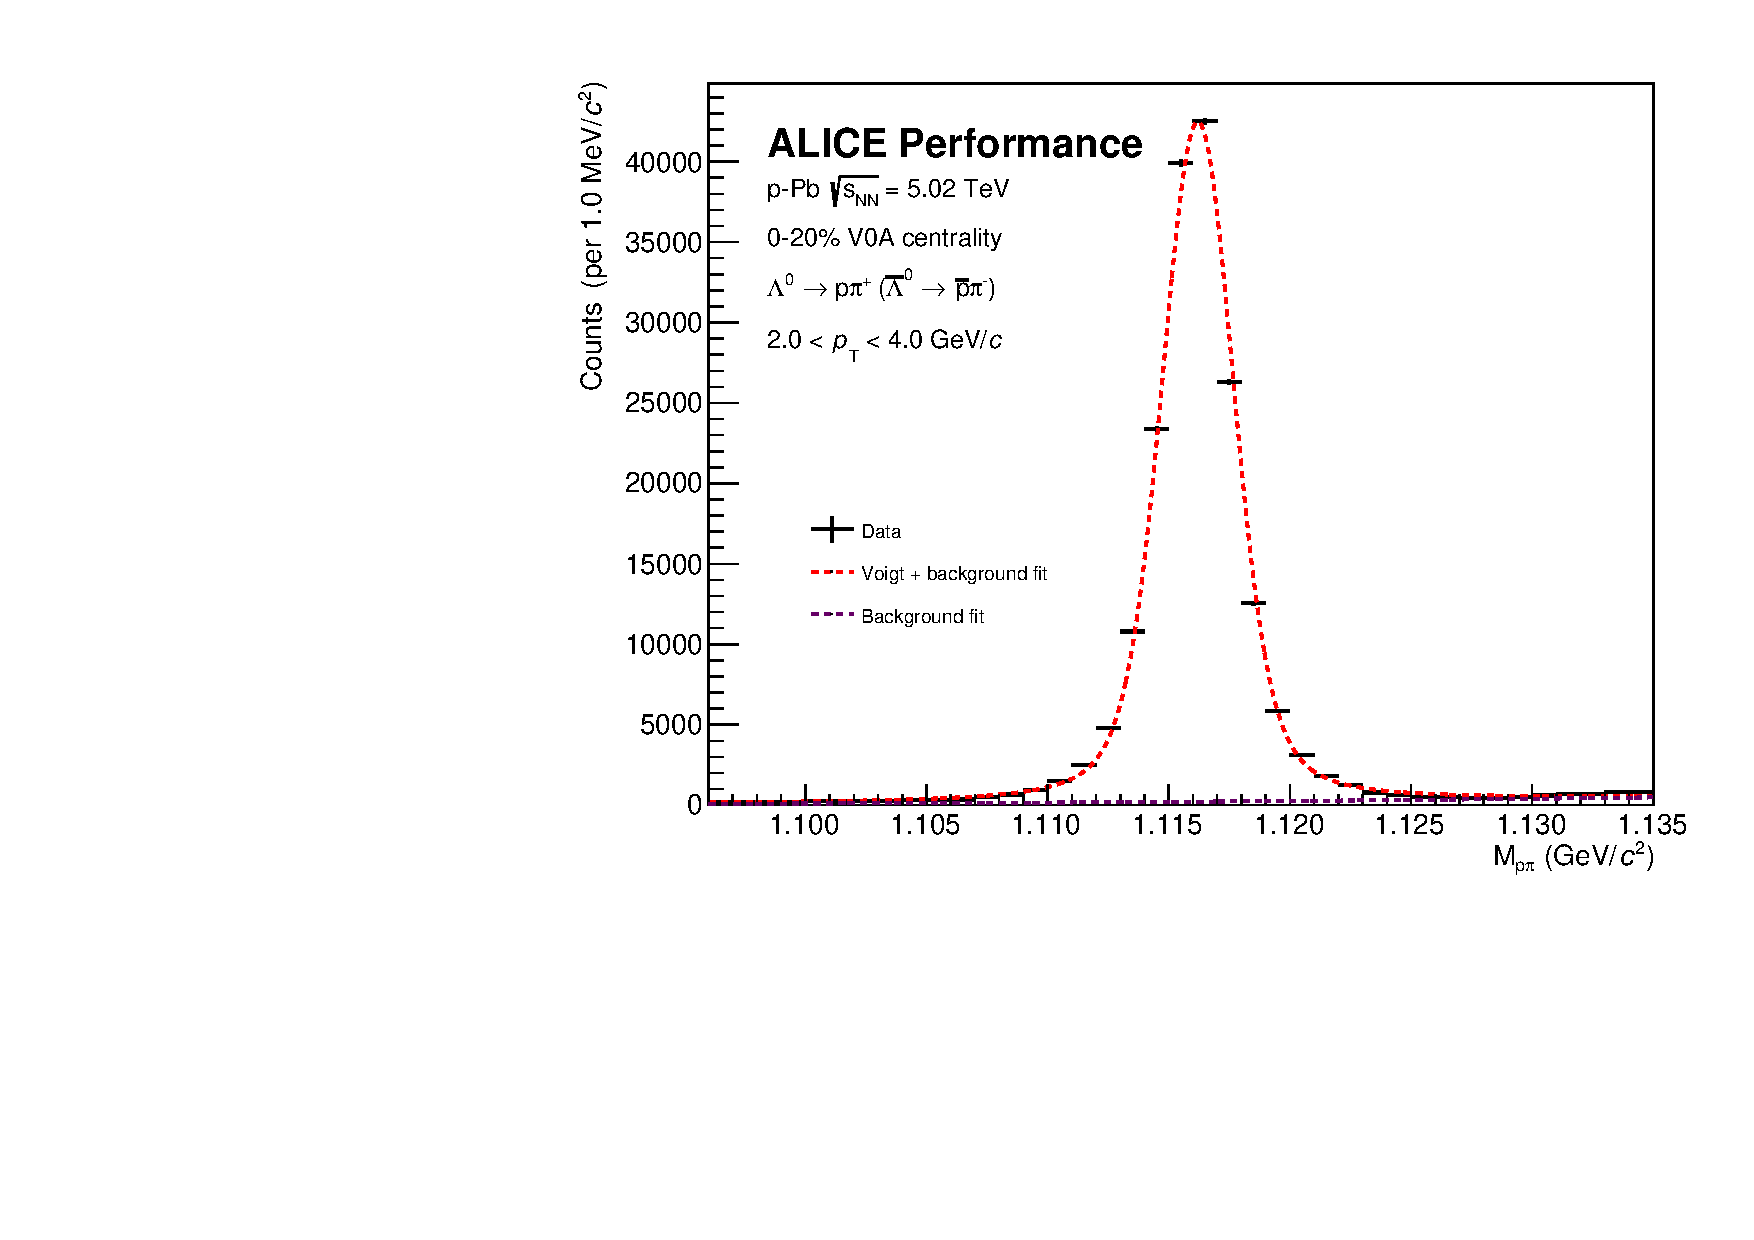
\includegraphics[width=2in]{figures/lambda_mass_0_20_v0_with_fit_zoomed.pdf}}
\end{subfigure}
\begin{subfigure} {
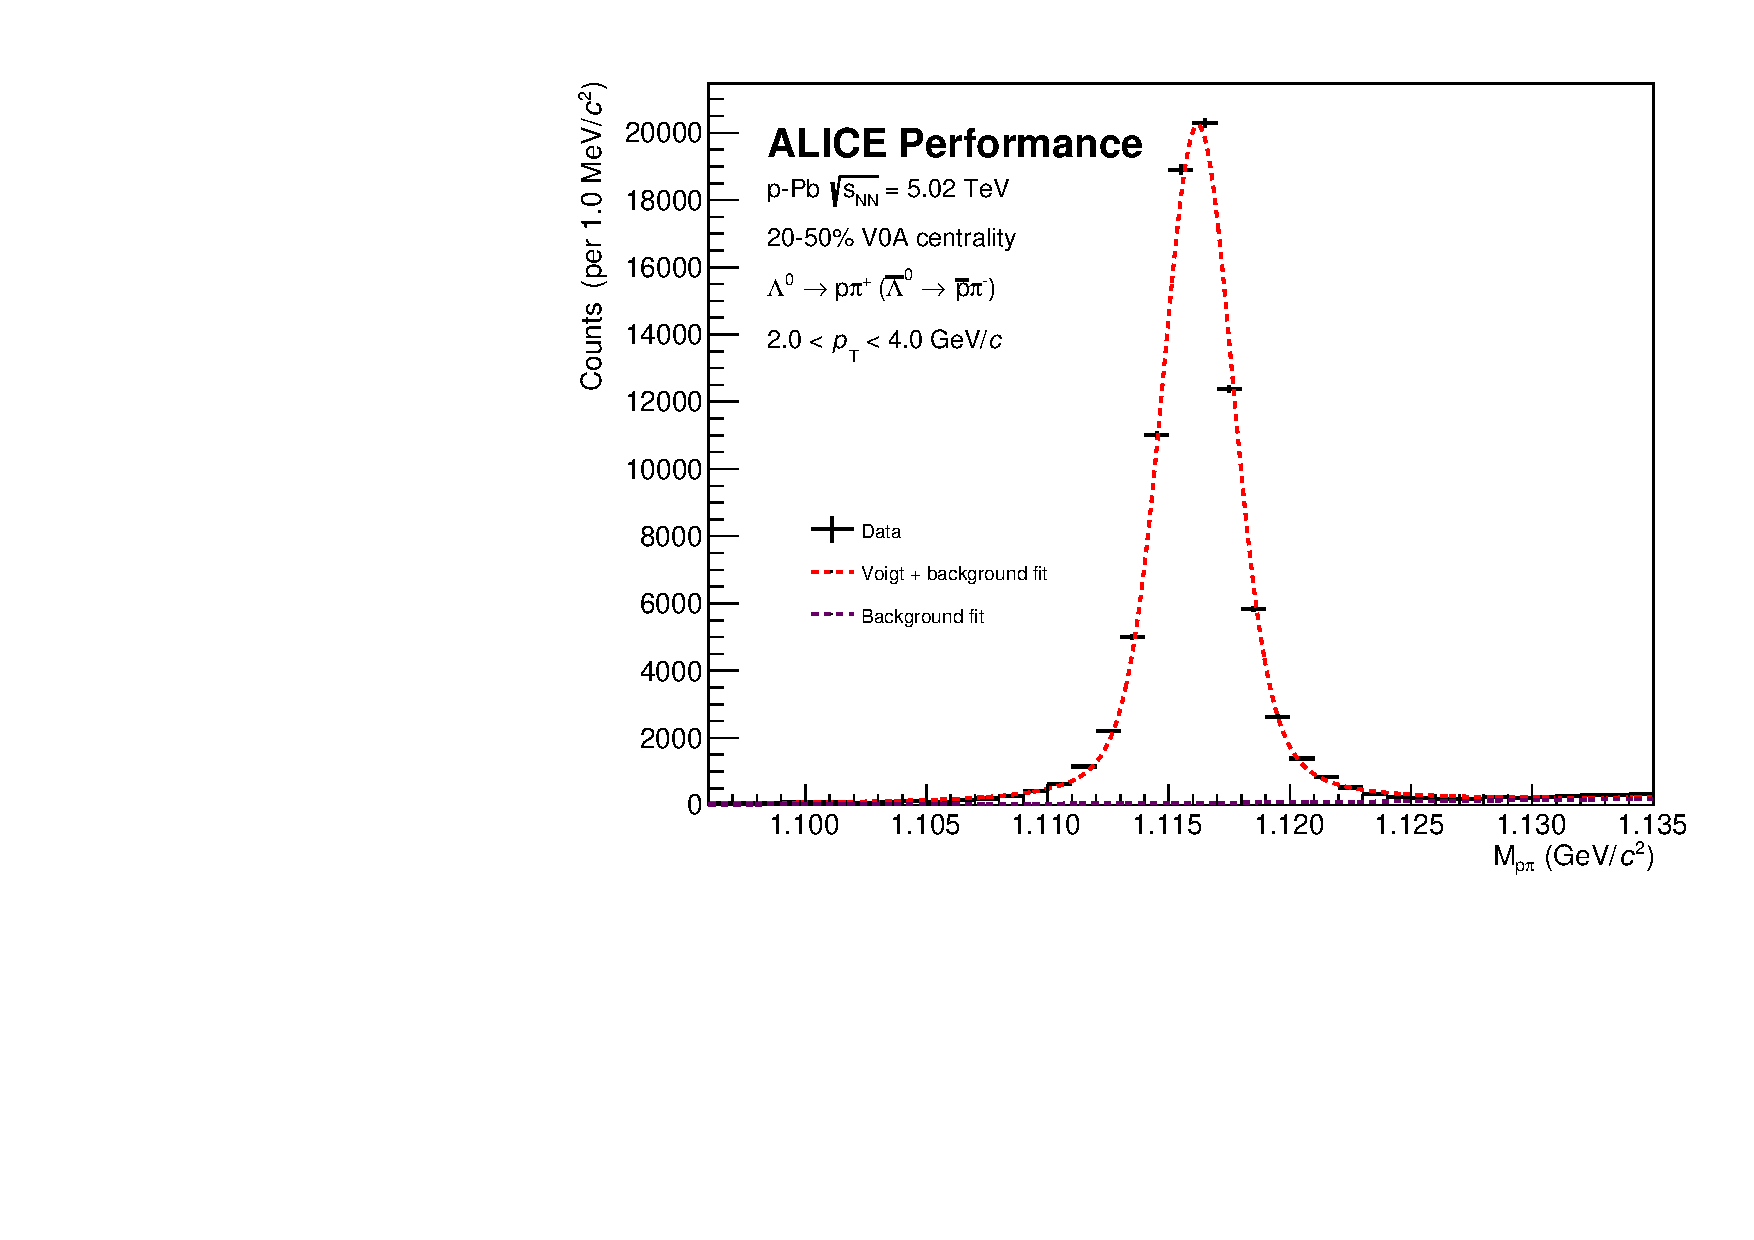
\includegraphics[width=2in]{figures/lambda_mass_20_50_v0_with_fit_zoomed.pdf}}
\end{subfigure}
\begin{subfigure} {
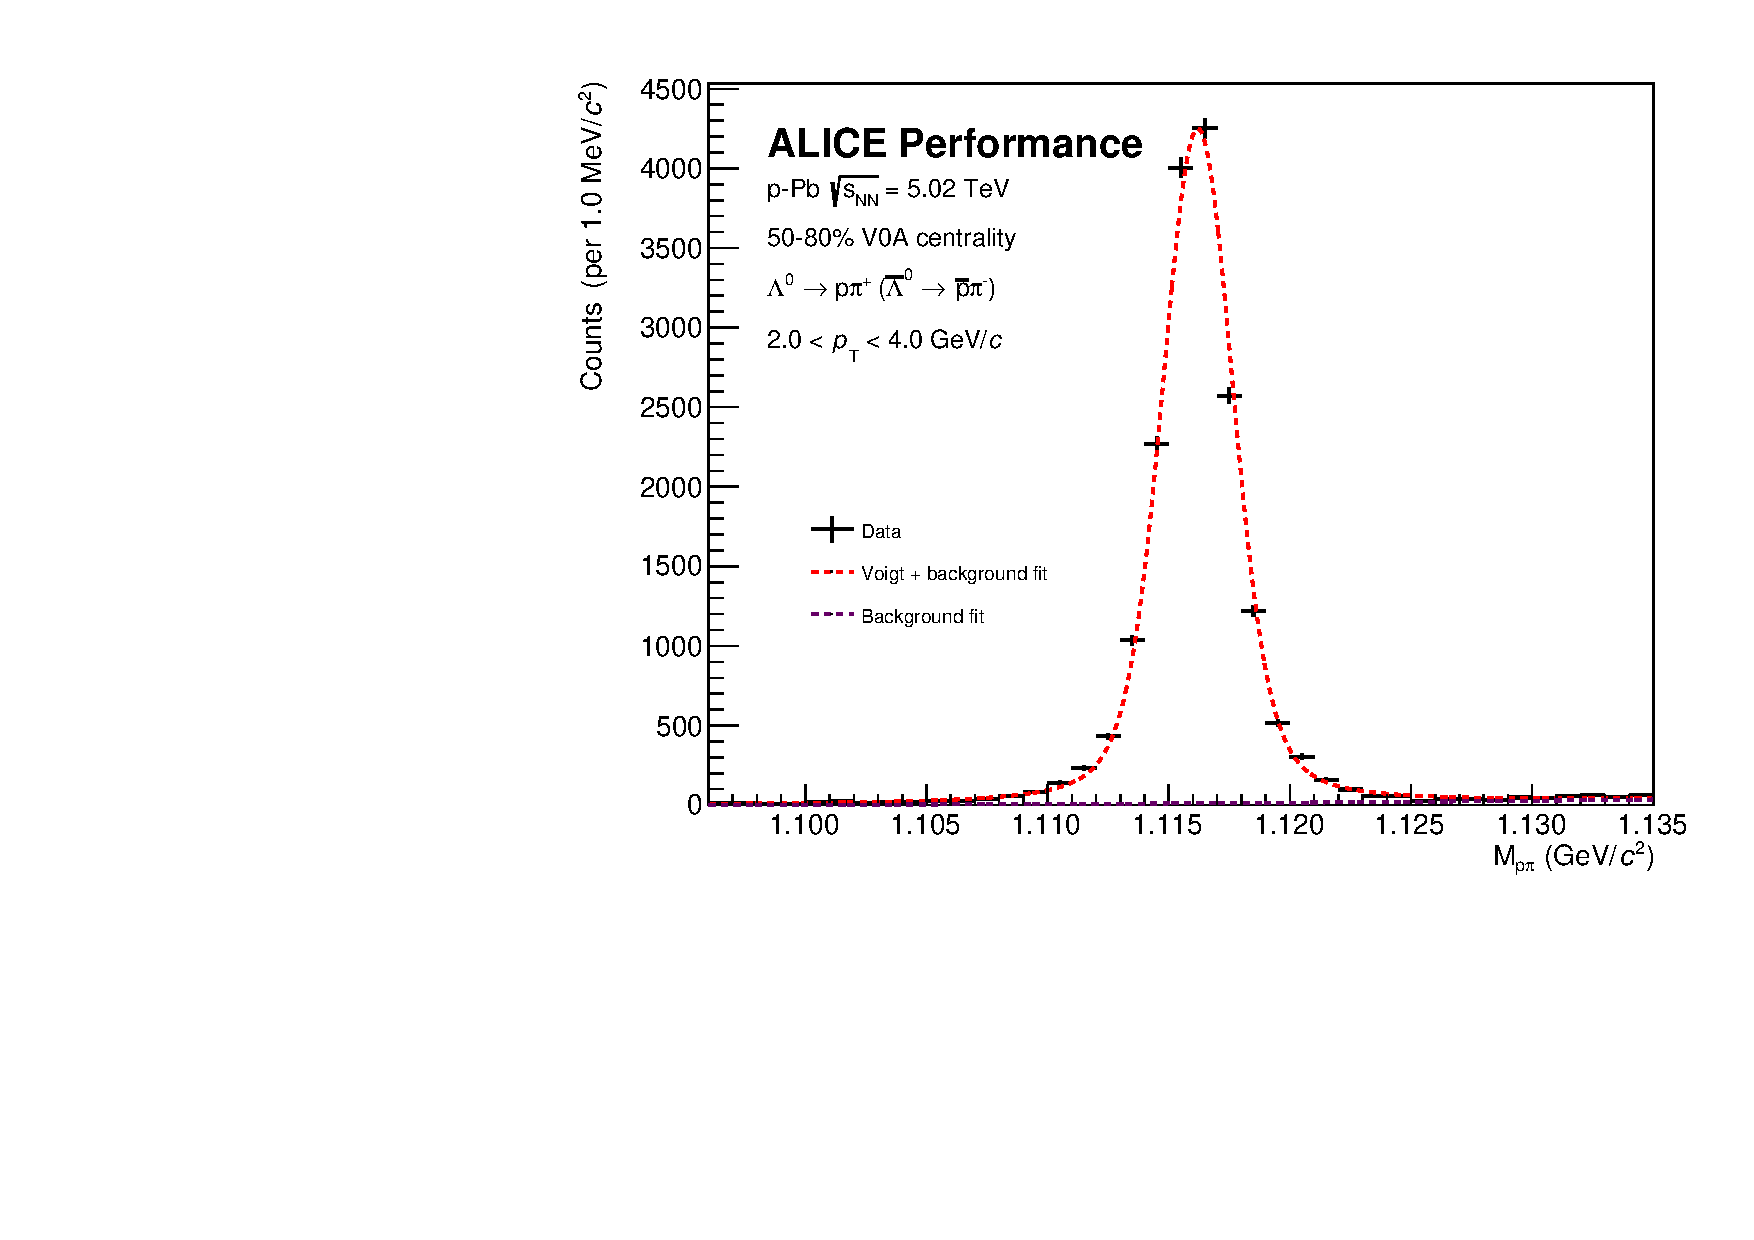
\includegraphics[width=2in]{figures/lambda_mass_50_80_v0_with_fit_zoomed.pdf}}
\end{subfigure}
\caption{Invariant mass distributions in the 0-20\% (left), 20-50\% (center), and 50-80\% (right) multiplicity bins for $\Lambda$s reconstructed using the V0 finder with $2 < \it{p}_T < 4$. The background from misidentified $\Lambda$s is negligible for all multiplicity bins, despite no topological cuts being applied to the V0s.}
\label{v0_mass}
\end{figure}

The relevant parameters for the Voigt fit applied to the invariant mass distributions for each multiplicy bin are shown in Table \ref{voigt_parameters}. While the background is nearly zero for each multiplciity bin, its effect on the final correlation measurement is investigated in Section \ref{systematics}.


 Measuring the $h-\Lambda$ correlation requires a clearly defined signal region for the unlike-sign $p\pi$ pairs from the V0 finder. The signal region range is as follows:

\begin{itemize}
	\item \makebox[7.5cm][l]{unlike-sign $p\pi$ in $\Lambda$ mass region:}  \SI{1.100}{GeV/c^2}$< M_{p\pi} < $\SI{1.134}{GeV/c^2}
\end{itemize}

This signal region was chosen to maximize statistical significance, and it does not depend on multiplicity. As it accounts for roughly ~99.5\% of the total signal, no correction for the tails of the distribution was applied. However, the choice of signal region and the corresponding correction factors are investigated more closely in Section \ref{systematics}.


\section{Correlation Measurement}
\label{corrsec}
\subsection{Full Correlation Measurement Method}

The per-trigger correlation is approximated using the formula:

\begin{align}
\label{perTrigEq}
C_{trig}(\Delta\varphi, \Delta\eta) = \frac{1}{N_{trig}}\frac{B(0,0)*S(\Delta\varphi,\Delta\eta)}{B(\Delta\varphi, \Delta\eta)}
\end{align}

where $S(\Delta\varphi, \Delta\eta)$ is the same event correlation and $B(\Delta\varphi, \Delta\eta)$ is the mixed-event correlation.  To properly account for the acceptance effects, the mixed-event distribution is scaled to the value of the $(\Delta\varphi = 0, \Delta\eta = 0)$ bin of the same event distribution. 


However, what is actually measured is an angular correlation of $h-(p\pi)$ pairs that is comprised of the real $h-\Lambda$ signal as well as a background of $h-(p\pi)$ pairs. The full correlation equation is then:

\begin{align}
\label{fullCorrEq}
\begin{split}
    C_{h-\phi}(\Delta\varphi, \Delta\eta) = r_{\text{Signal}}\biggl(&C_{(h-p\pi)^{US}_{\text{Signal}}}(\Delta\varphi, \Delta\eta)\\
    &- r_{LS}*C_{(h-p\pi)^{US}_{\text{RSB}}}(\Delta\varphi, \Delta\eta)\biggr)
\end{split}
\end{align}

Here, $r_{\text{Signal}}$ accounts for the signal that is missed by choosing a finite signal region, and is calculated using the Voigt fit discussed in Section \ref{invariant_mass_region} by dividing the integral of the fit across the entire range by the integral of the fit in the signal region. For our central values, this fraction is nearly unity and is thus not included in the final correlation measurement. $r_{LS}$ is a scaling factor that depends on the technique used to account for the $p\pi$ background and is discussed further in Sections \ref{systematics} and \ref{resonance_technique}.


While the $h-(p\pi)$ background is negligible within our main transverse momentum bin ($2 < \it{p}_{T} < 4$) for $\Lambda$s reconstructed using the V0 finder, the full correlation formula is still used in this analysis and is discussed further in Sections \ref{systematics} and \ref{resonance_technique}.

\subsection{Mixed Event Acceptance Correction}

For each multiplicity bin, events were separated into z-vertex position bins with a width of \SI{2}{cm}, ranging from \SI{-10}{cm} to \SI{10}{cm}. An AliEventPool of size 500 and track-depth 1000 was filled with a list of trigger tracks, then correlated with a list of associated hadrons (or $p\pi$ pairs) for each event once the pool was ready. The uncorrected and mixed-event distributions (h-$p\pi$, h-h) in the 0-20\% multiplicity bin are shown in Figures \ref{uncorr2d_0_20} and \ref{mixed2d_0_20}, respectively.

\begin{figure}[ht]
\centering
\begin{subfigure}{
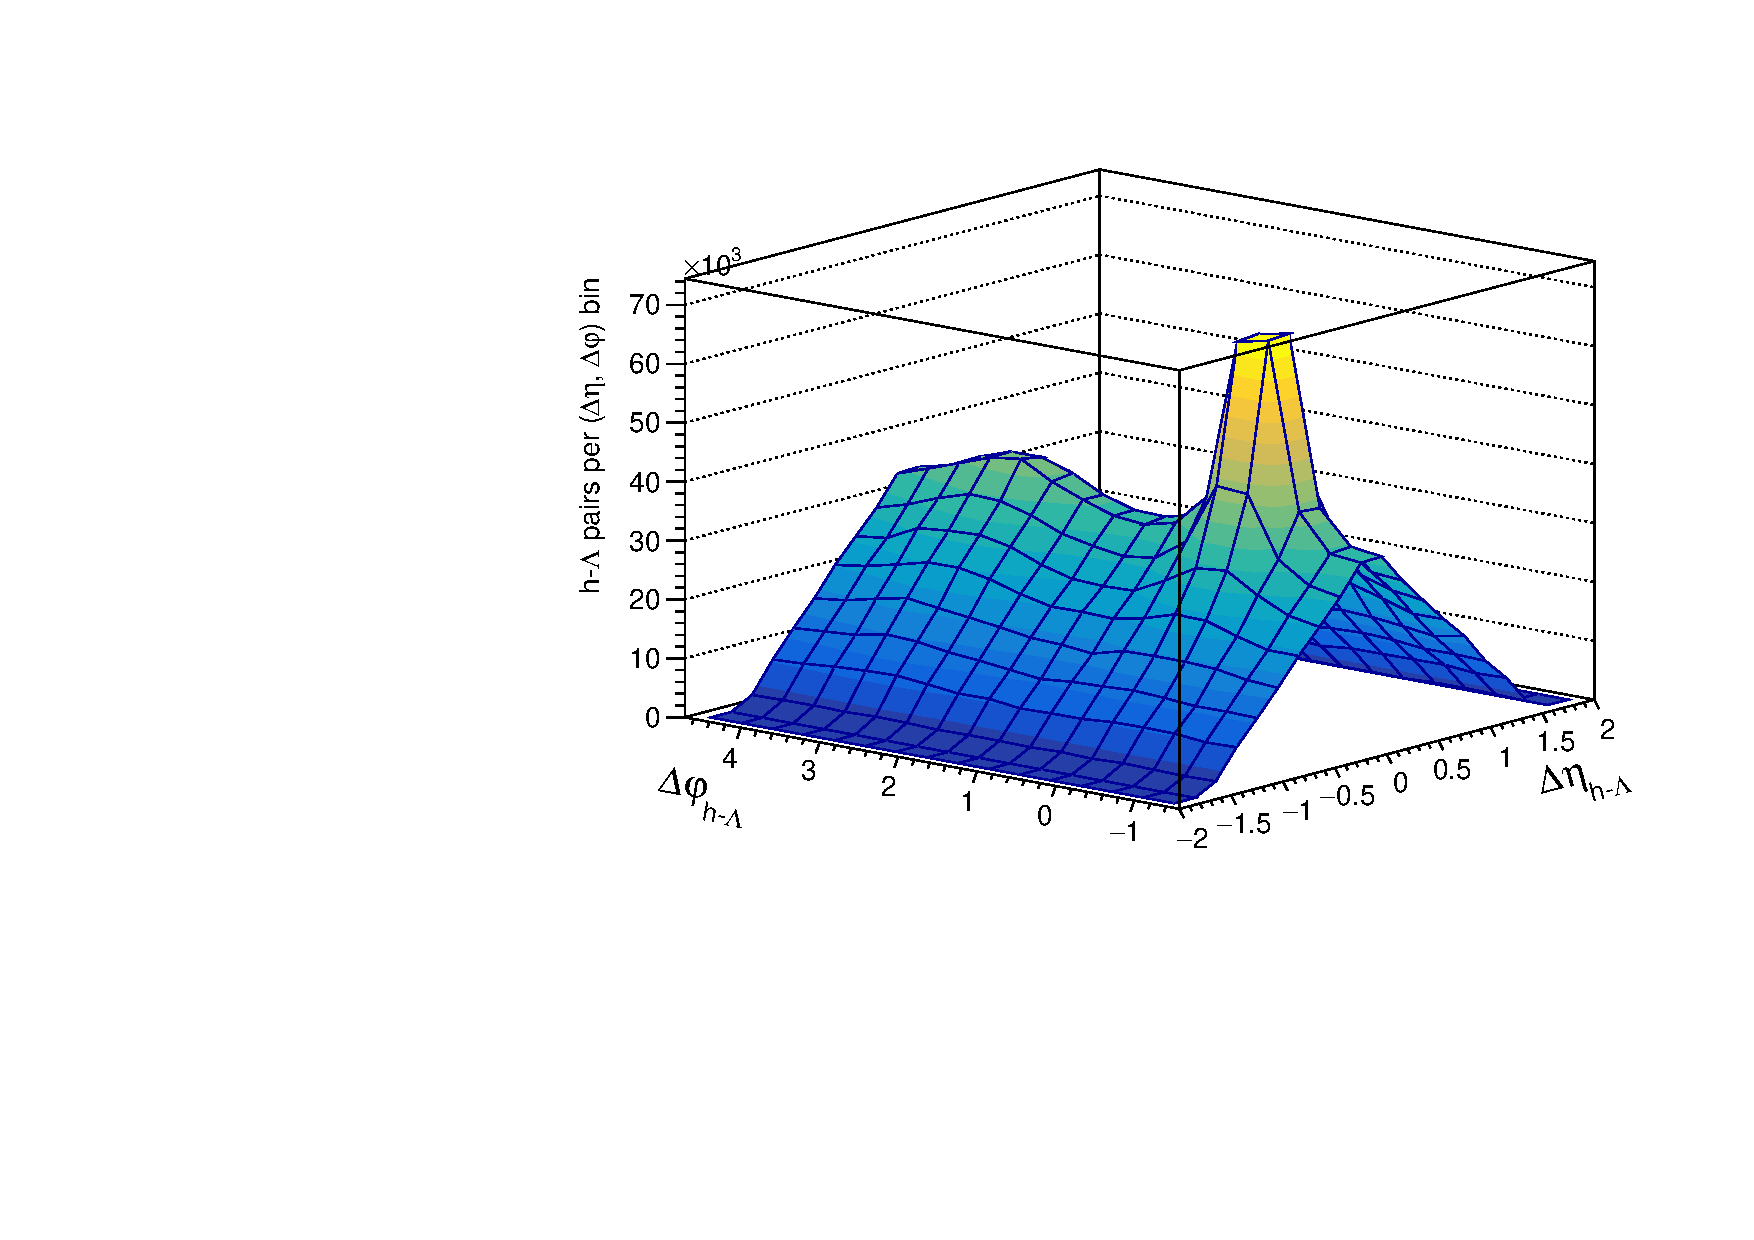
\includegraphics[width=3in]{figures/h_lambda_2d_nomixcor_0_20.pdf}}
\end{subfigure}
\begin{subfigure}{
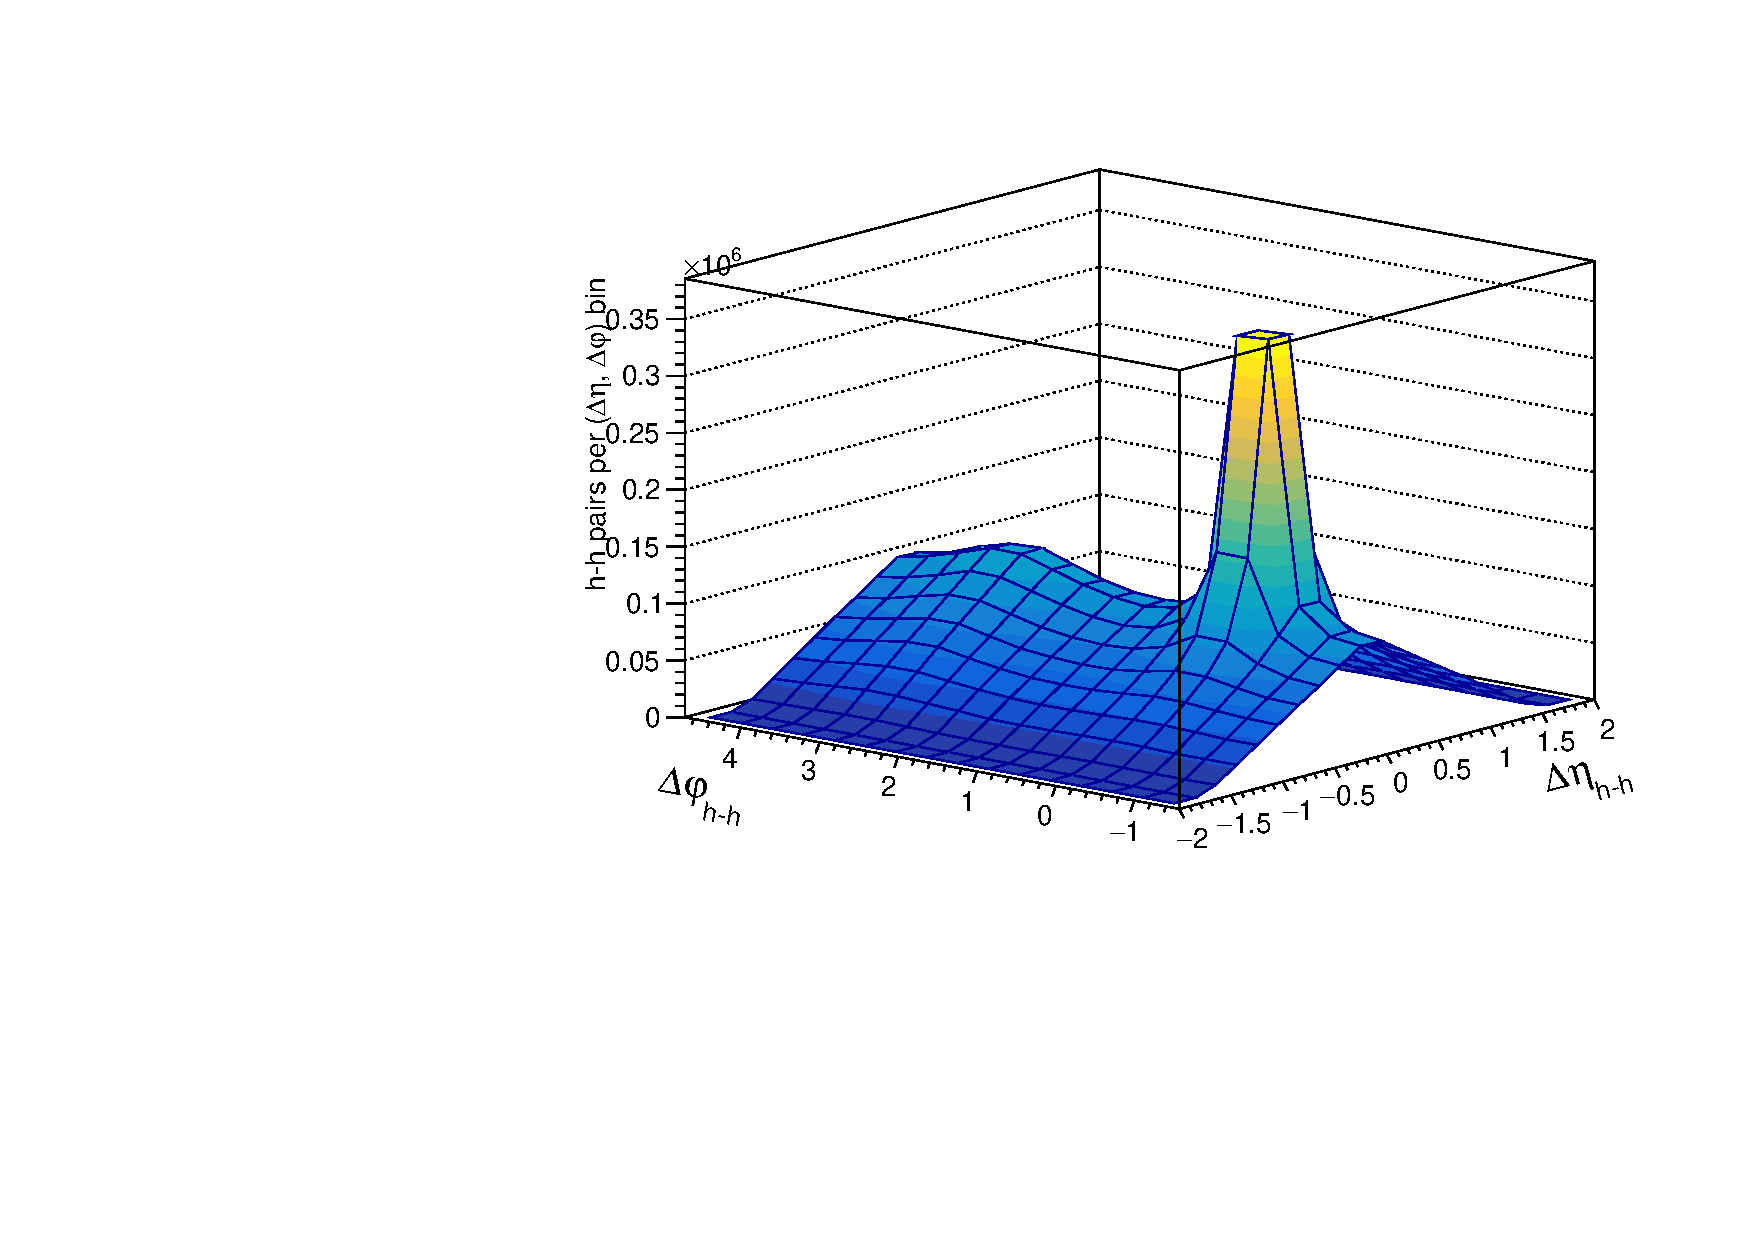
\includegraphics[width=3in]{figures/h_h_2d_nomixcor_0_20.pdf}}
\end{subfigure}
\caption{2-D non-acceptance corrected h-$p\pi$ (left) and h-h (right) angular correlations for the 0-20\% multiplicity bin (all z-vertex bins merged together)}
\label{uncorr2d_0_20}
\end{figure}

\begin{figure}[ht]
\centering
\begin{subfigure}{
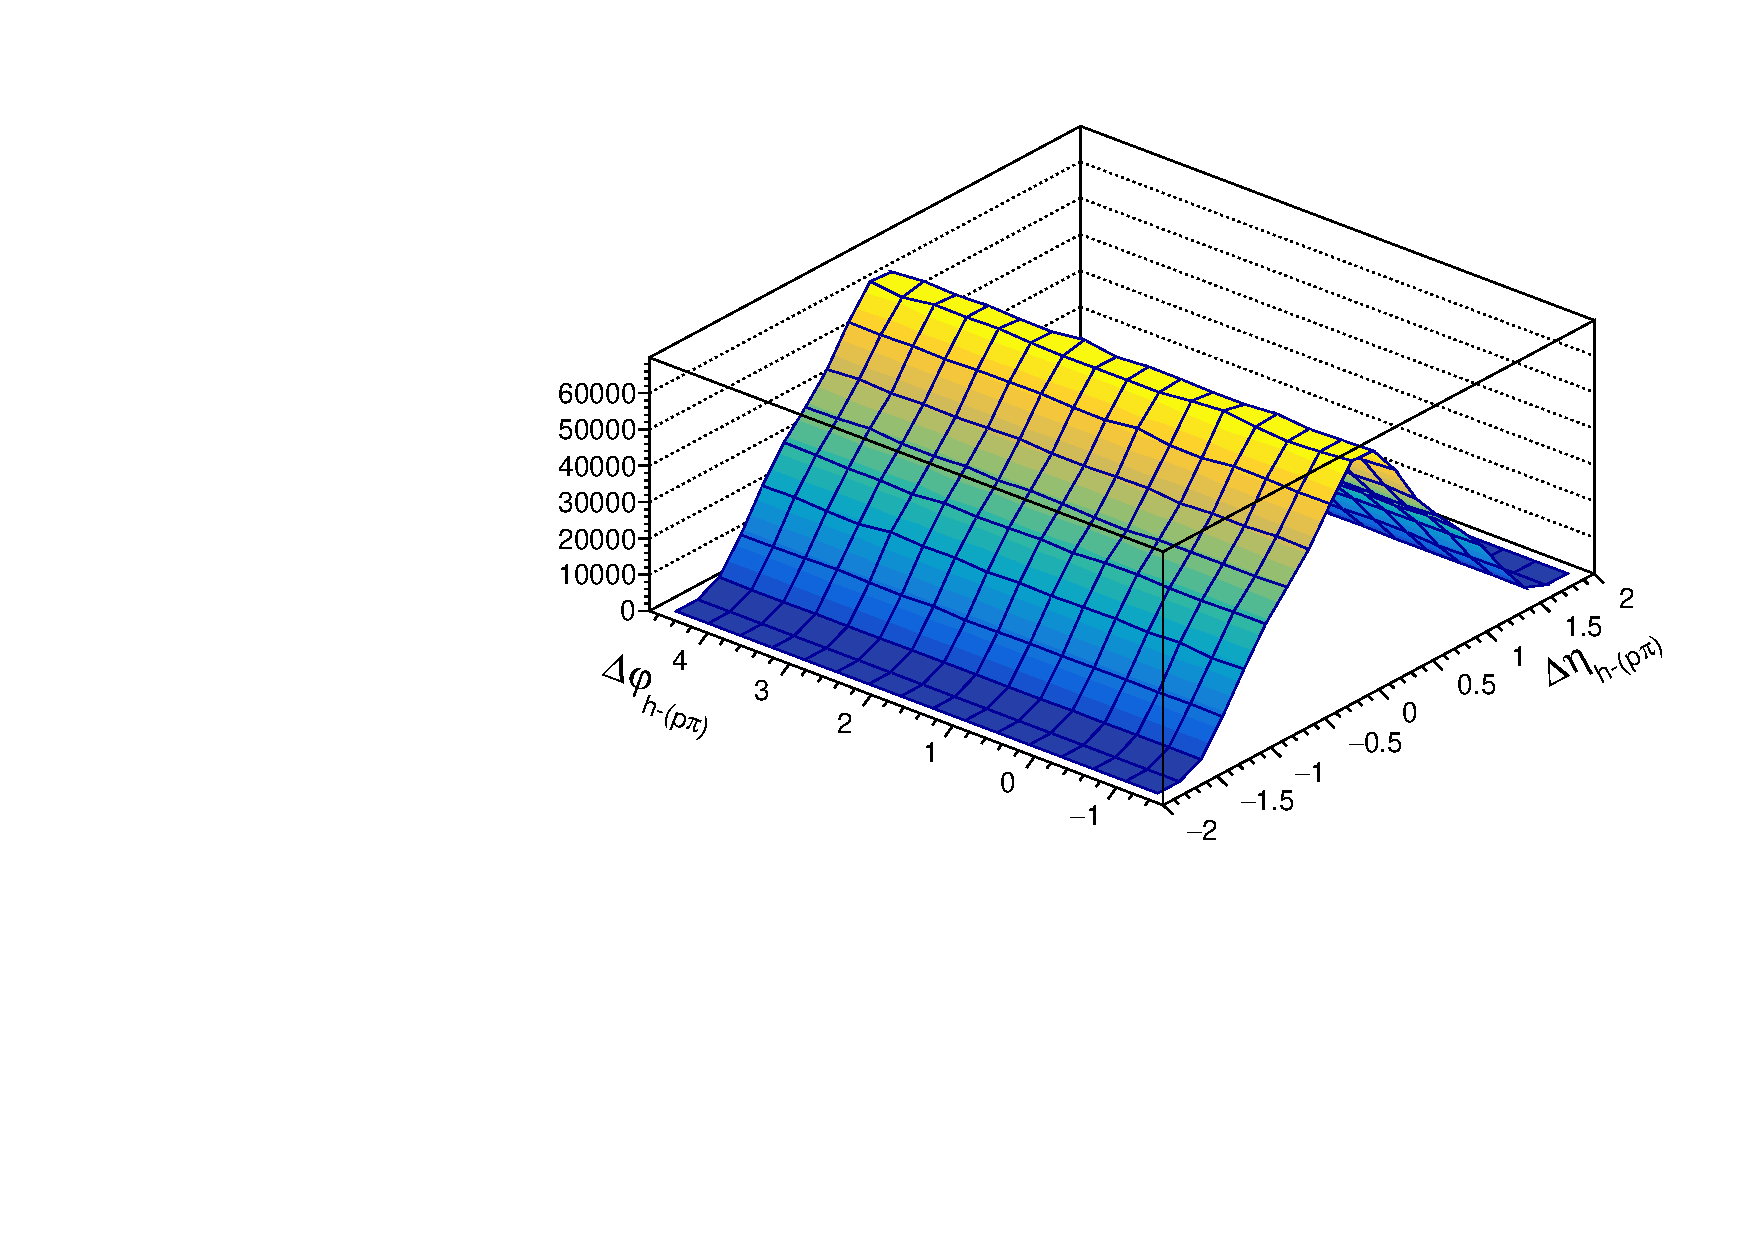
\includegraphics[width=3in]{figures/h_lambda_2d_mixed_0_20.pdf}}
\end{subfigure}
\begin{subfigure}{
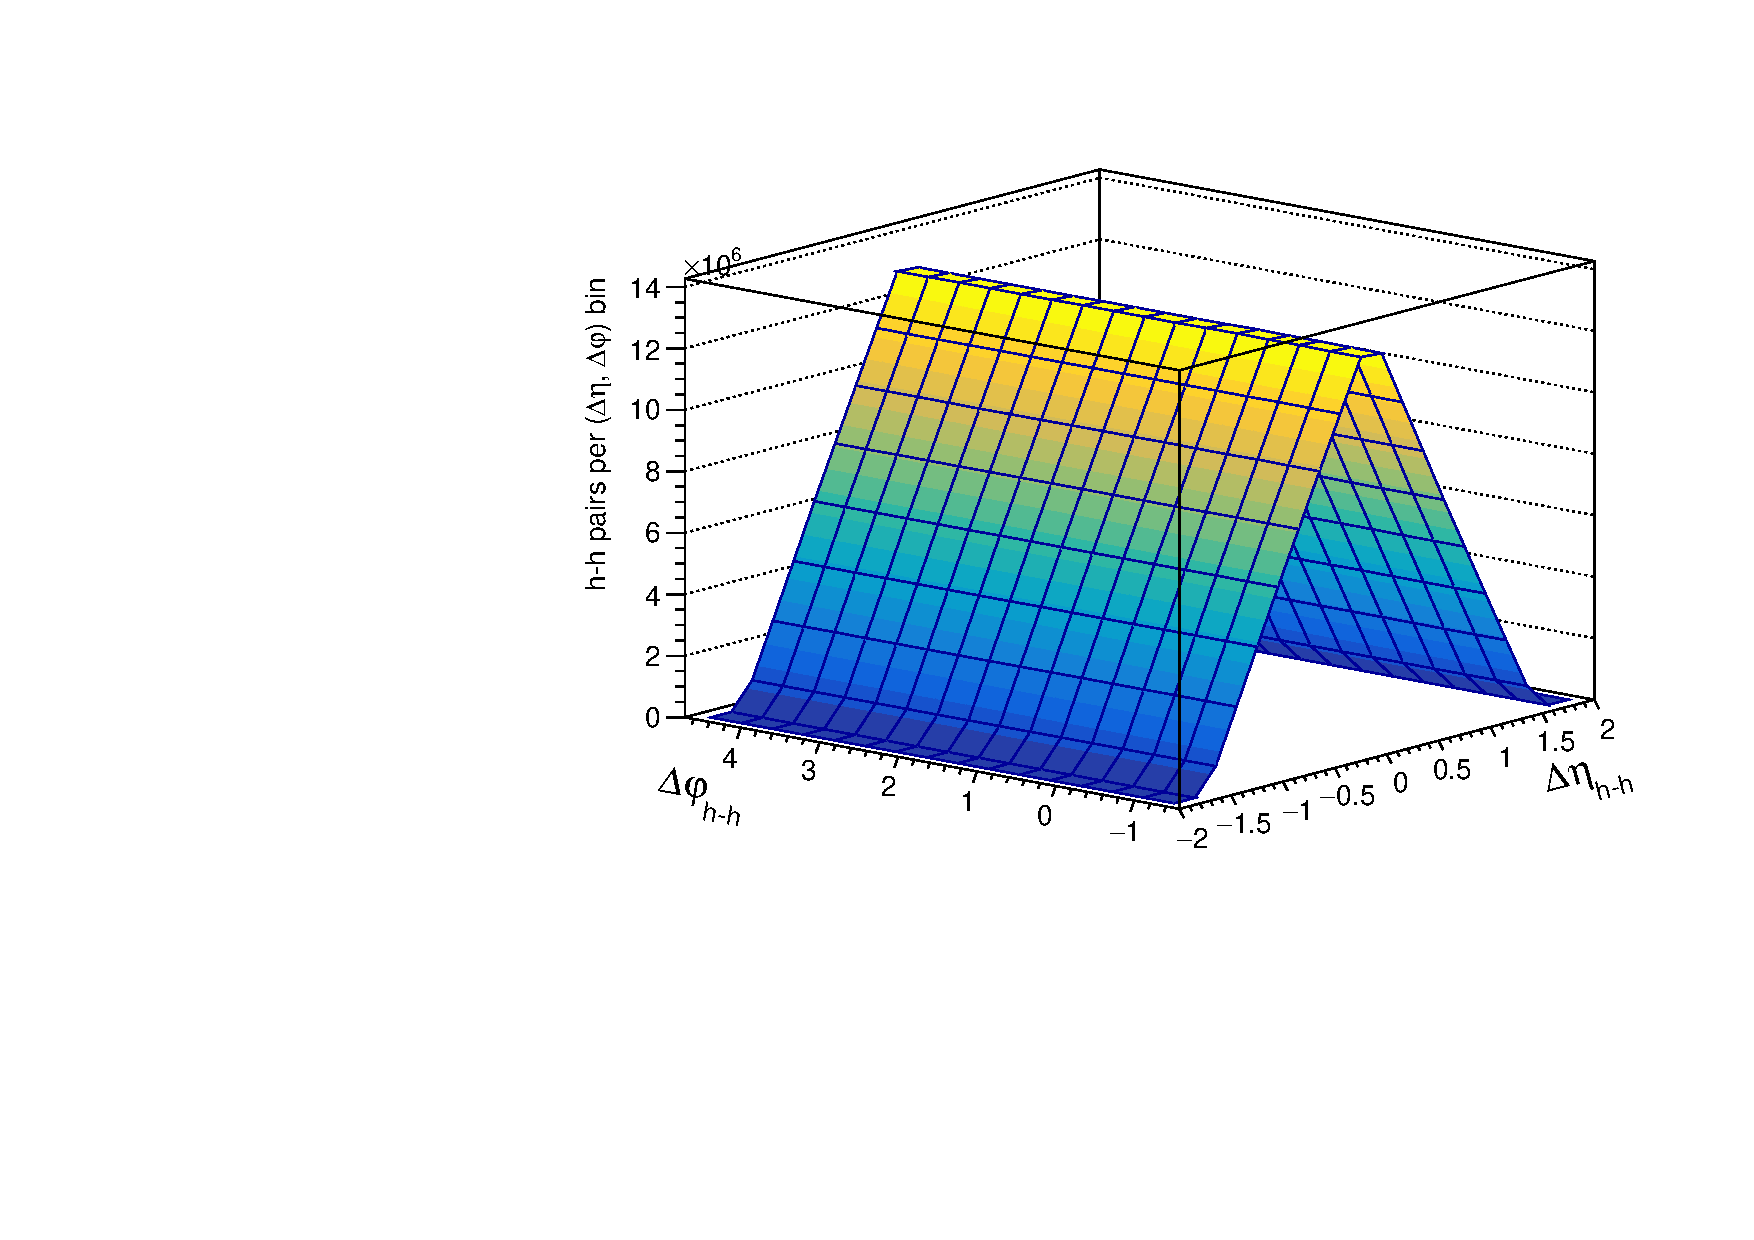
\includegraphics[width=3in]{figures/h_h_2d_mixed_0_20.pdf}}
\end{subfigure}
\caption{2-D mixed event h-$p\pi$ (left) and h-h (right) angular correlations for the 0-20\% multiplicity bin (all z-vertex bins merged together)}
\label{mixed2d_0_20}
\end{figure}

For each multiplicity bin, the acceptance correction (as described in Eq. 1) was performed for each z-vertex bin, then the results were merged together to form the acceptance-corrected distributions, shown in Figure \ref{mixcor2d}. 

\begin{figure}[ht]
\centering
\begin{subfigure}{
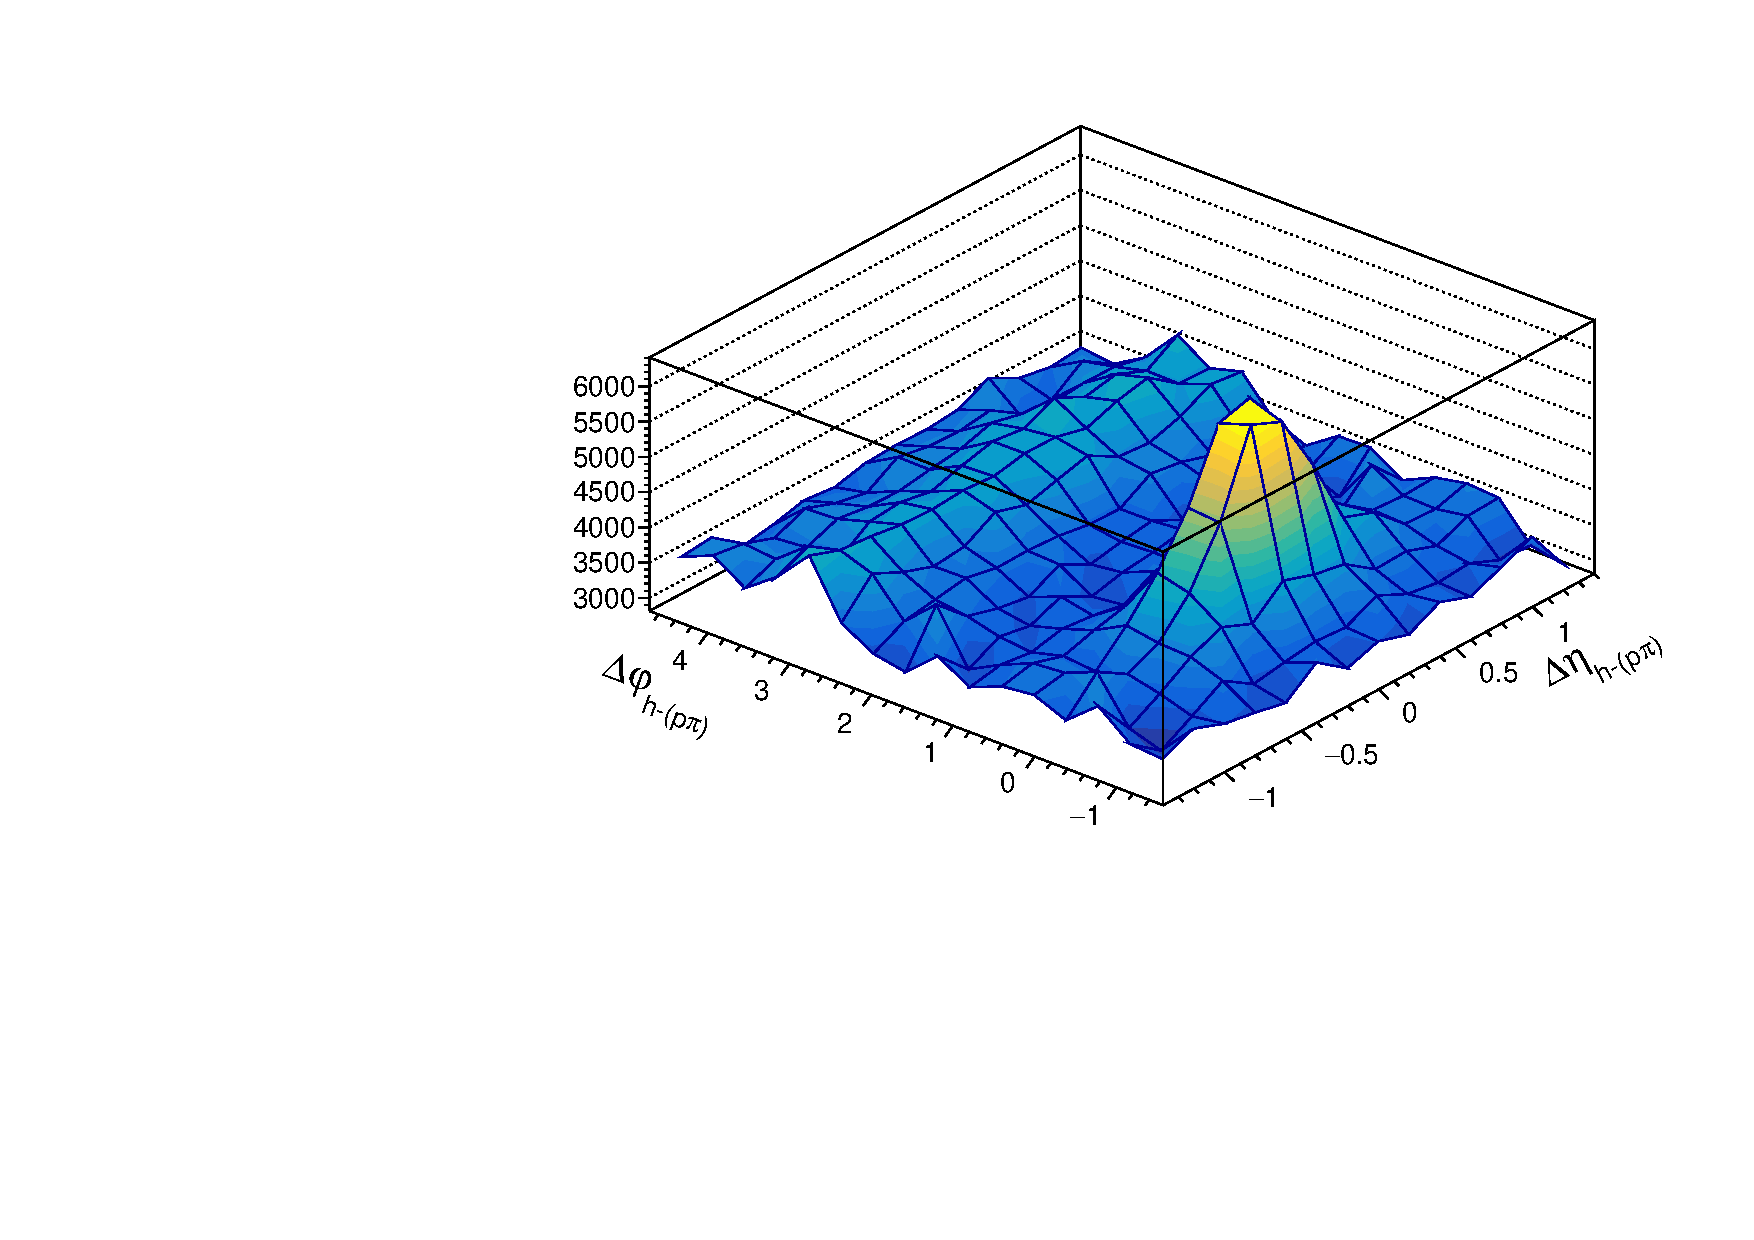
\includegraphics[width=3in]{figures/h_lambda_2d_mixcor_0_20.pdf}}
\end{subfigure}
\begin{subfigure}{
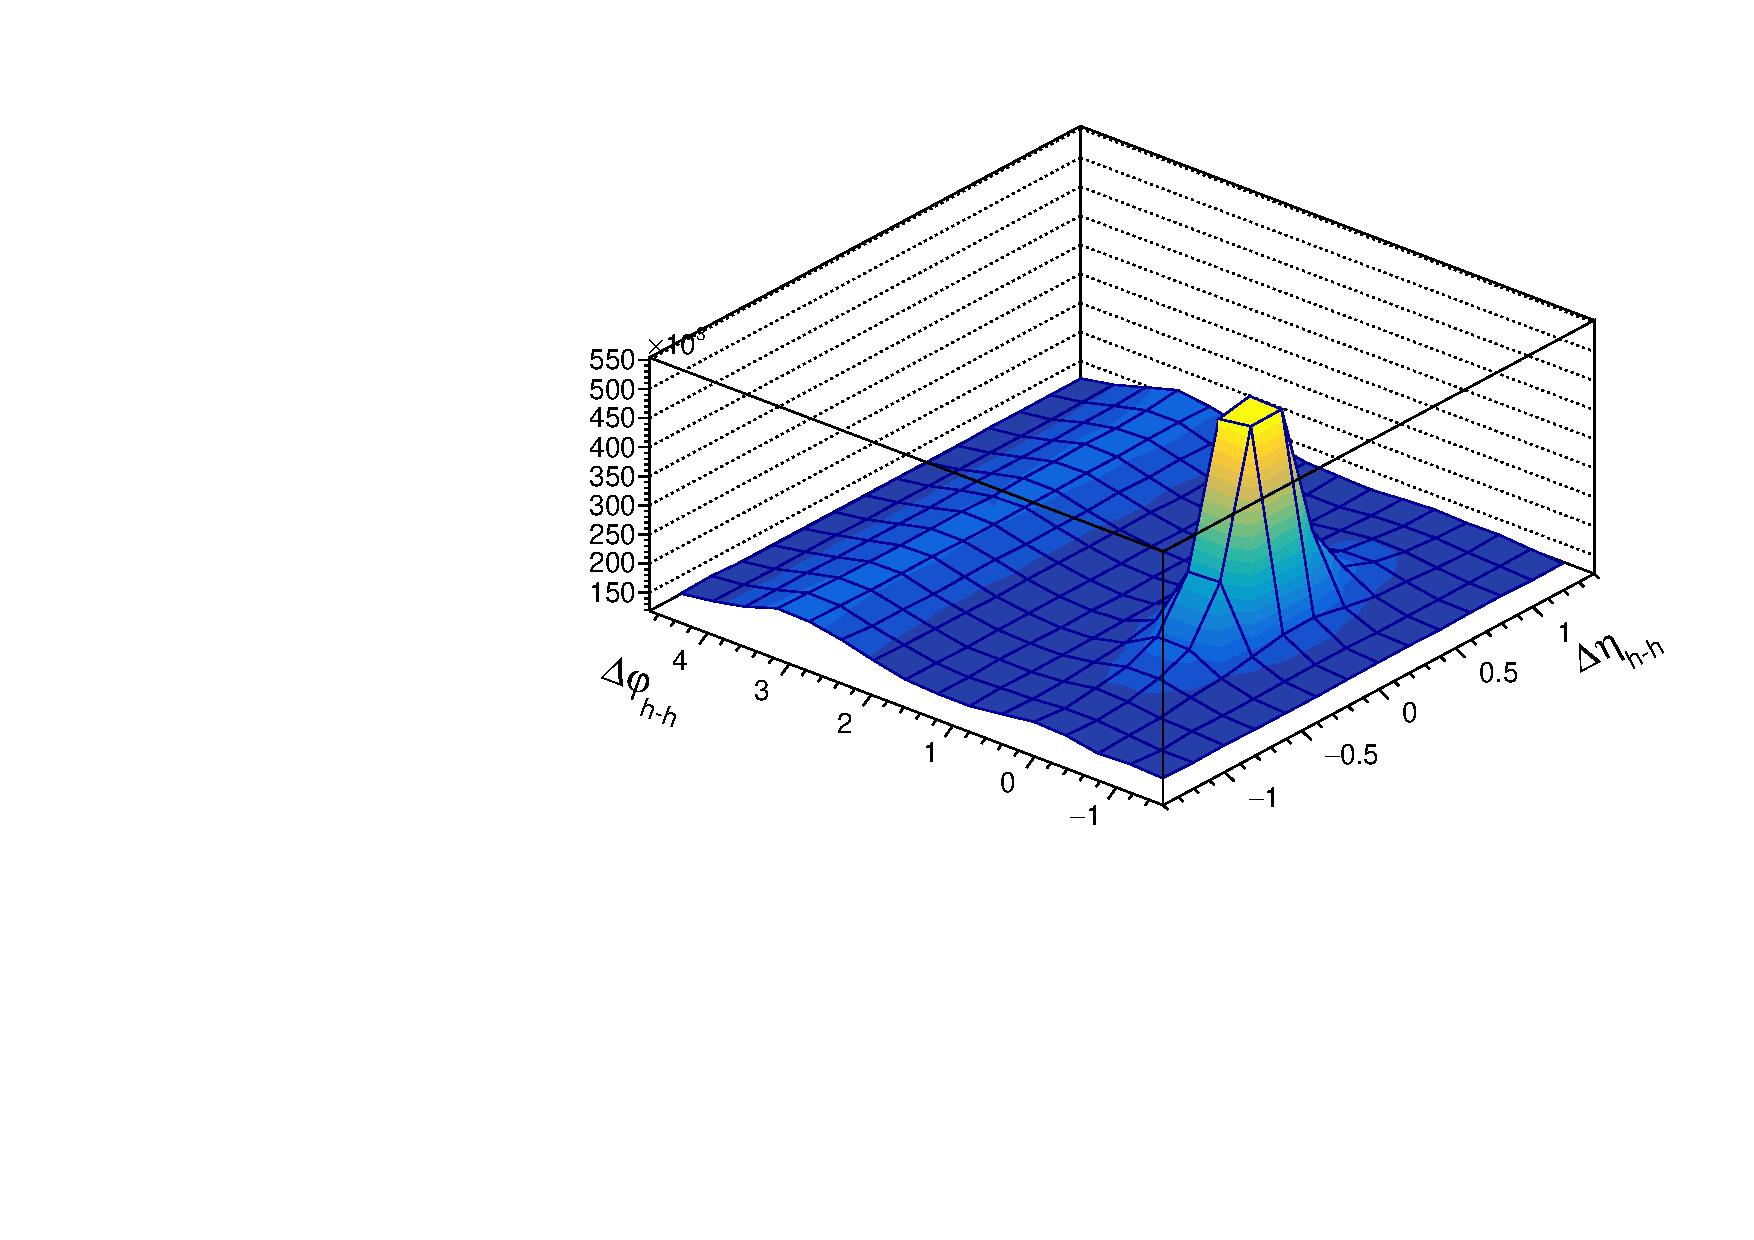
\includegraphics[width=3in]{figures/h_h_2d_mixcor_0_20.pdf}}
\end{subfigure}
\caption{2-D h-$p\pi$ (left) and h-h (right) angular correlations for the 0-20\% multiplicity bin after acceptance corrections. Note that the triangular shape in $\Delta\eta$ is no longer present.}
\label{mixcor2d_0_20}
\end{figure}

As this analysis relies on multiple angular correlations ($h-\Lambda$, $h-h$), the event mixing was done with a shared mixed event pool containing the list of trigger tracks, then the correlation was performed using the associated ($p\pi$) or hadron list for each event. After mixing, each correlation was corrected using its corresponding mixed-event distribution. The event mixing was only performed on events that contained both a $\Lambda$ candidate ($p\pi$ pair from either V0 finder or global AOD list) and an associated hadron.

\subsection{Reconstruction Efficiency}
\label{reconstruction_efficiency}

\subsubsection{$\Lambda$ Reconstruction Efficiency}
\label{lambda_efficiency}

To estimate the $\Lambda$ reconstruction efficiency, we compare $\Lambda$ yields reconstructed using the V0 finder to the true $\Lambda$ yields using the MC production LHC17f2b\_FAST (anchored to LHC16q\_FAST production). The efficiency was calculated using the following formula:

\begin{align*}
	\varepsilon_{\Lambda} &=  \frac{N_{\Lambda\text{, reco with V0 finder}}}{N_{\Lambda\text{, real MC yield}}},
\end{align*}

where each $\Lambda$ in $N_{\Lambda\text{, reco with V0 finder}}$ meets the following criteria:

\begin{itemize}
	\item Found in the list of offline V0s
	\item $|\eta_{V0}| \leq 0.8$
	\item The daughter $p, \pi$ pass the daughter track cuts outlined in Section \ref{daughtercuts}
	\item The daughter $p, \pi$ tracks have corresponding real $p, \pi$ in the MC stack
	\item The corresponding MC stack $p, \pi$ daughters come from the same mother $\Lambda$ (also in MC stack)
\end{itemize}

and each $\Lambda$ in $N_{\Lambda\text{, real MC yield}}$ meets the following criteria:

\begin{itemize}
	\item Found in the MC stack
	\item $|\eta_{\Lambda}| \leq 0.8$
	\item The $\Lambda$ decays to $p\pi$
\end{itemize}

While previous analyses focus solely on primary $\Lambda$s (exlcuding $\Omega$ and $\Xi$ contamination), there is no requirement for either the V0-reconstructed $\Lambda$ or the MC-generated $\Lambda$ to be a primary particle. As this analysis is mostly interested in the $\Lambda$ due to its strange quark content, whether or not the $\Lambda$ came from a cascade decay is irrelevant. This is important to note when making comparisons between this analysis and previous analyses, as secondary contamination from cascades accounts for nearly 20\% of all $\Lambda$s.

As mentioned in Section \ref{lambda_reconstruction}, both the $\Lambda$ and the $\bar{\Lambda}$ were combined together for this efficiency calculation. Efficiencies were calculated as a function of $p_T$, $\eta$, $\varphi$, Event Z vertex, and Multiplicity. Similarly to previous efficiency studies in 2013 pPb data, no significant dependency of efficiency on multiplicity was found (fig. \ref{oldeff}). The final efficiency correction was applied as a function of $p_T$ only.

\begin{figure}[ht]
\centering
\begin{subfigure}{
\includegraphics[width=3in]{images/myeff_pT.pdf}}
\end{subfigure}
\begin{subfigure}{
\includegraphics[width=3in]{images/2013_efficiency_analysisnote.pdf}}
\end{subfigure}
\caption{Efficiency vs. $p_T$ for $\phi$ meson reconstruction.  \textbf{Left:} New results for this study using LHC17f2b\_FAST MC dataset anchored to LHC16q\_FAST. \textbf{Right:} Old results using 2013 pPb data.  There is qualitative agreement between the 2013 and new 2016 calculated efficiency, and in both cases, there is no significant dependence on multiplicity.}
\label{oldeff}
\end{figure}

\subsection{Trigger and Associated Hadron Reconstruction Efficiency}
\label{trigassoc_efficiency}

The trigger and associated hadron reconstruction efficiencies are calculated using the following formula:

\begin{align*}
	\varepsilon_{trig, assoc} &=  \frac{N_{trig, assoc\text{, reco yield}}}{N_{trig, assoc\text{, real MC yield}}},
\end{align*}

where each trigger or associated hadron in $N_{trig, assoc\text{, reco yield}}$ meets the following criteria:

\begin{itemize}
	\item Found in the list of AOD tracks
	\item $|\eta_{track}| \leq 0.8$
	\item The track passes the track cuts outlined in Section \ref{trigcuts} (trigger) or \ref{assoccuts} (associated)
	\item The track has a corresponding real track in the MC stack
	\item The corresponding MC track is either a pion, proton, kaon, electron or muon
	\item The corresponding MC track is not a secondary particle (IsPhysicalPrimary() == true)
\end{itemize}

and each trigger or associated hadron in $N_{trig, assoc\text{, real MC yield}}$ meets the following criteria:

\begin{itemize}
	\item Found in the MC stack
	\item $|\eta_{track}| \leq 0.8$
	\item The track is either a pion, proton, kaon, electron or muon
	\item The track is not a secondary particle (IsPhysicalPrimary() == true)
\end{itemize}

The efficiencies for both the trigger and associated hadrons as a function of $\it{p}_T$ are shown in Figure \ref{trigassoc_eff_plots}.

\begin{figure}[ht]
\centering
\begin{subfigure}{
\includegraphics[width=3in]{images/myeff_pT.pdf}}
\end{subfigure}
\begin{subfigure}{
\includegraphics[width=3in]{images/2013_efficiency_analysisnote.pdf}}
\end{subfigure}
\caption{Efficiency vs. $p_T$ for $\phi$ meson reconstruction.  \textbf{Left:} New results for this study using LHC17f2b\_FAST MC dataset anchored to LHC16q\_FAST. \textbf{Right:} Old results using 2013 pPb data.  There is qualitative agreement between the 2013 and new 2016 calculated efficiency, and in both cases, there is no significant dependence on multiplicity.}
\label{oldeff}
\end{figure}

As our correlation measurement depends on both the trigger and associated particle, we must combine the two efficiencies to get the overall efficiency for the pair.  This is done using the following formula:

\begin{align*}
    \epsilon_{pair} = \epsilon_{trig}*\epsilon_{assoc}
\end{align*}

This efficiency is corrected for on-the-fly as the pairs are being filled into the total correlation distribtuion by using a weighting factor equal to the inverse of $\epsilon_{pair}$. The same trigger efficiency used in the pair efficiency is then also to correct our $N_{trig}$ for our final per-trigger correlation in both the h-h and h-$\Lambda$ case.



\subsection{Removal of Combinatorial K-K Background}
\label{removecomb}

Since we have no a priori knowledge of which kaon pairs came from a real $\phi$ decay, we must remove the contribution to the angular correlation structure due to the combinatorial background of random kaon pairs.

To do this, h-(KK) angular correlations are measured for un-likesign kaon pairs in two invariant mass sideband regions (fig. \ref{sidebands}).  The correlation structures in these regions are then normalized and averaged together to give an estimate of the combinatorial background shape.  The self-normalized 1D $\Delta\varphi$ correlations in the two sideband regions are shown in figure \ref{normSBcorr}, showing that within statistical fluctuations they have identical correlation shapes.

\begin{figure}[ht]
\centering
\begin{subfigure}{
\includegraphics[width=3in]{images/narrowmass_withSB_invmass.pdf}}
\end{subfigure}
\begin{subfigure}{
\includegraphics[width=3in]{images/dphi_masspeak.pdf}}
\end{subfigure}
\begin{subfigure}{
\includegraphics[width=3in]{images/dphi_LSB.pdf}}
\end{subfigure}
\begin{subfigure}{
\includegraphics[width=3in]{images/dphi_RSB.pdf}}
\end{subfigure}
\caption{Correlations are measured for three different regions of un-like sign Kaon pair Mass: the left sideband, the mass peak region, and the right sideband (colored regions of invariant mass plot). Each of these correlations are separately corrected for acceptance effects using Mixed-Event techniques. The final $h-\phi$ Correlation is calculated by taking the "mass peak" correlation, and subtracting a scaled average of the two sideband regions.}
\label{sidebands}
\end{figure}

\begin{figure}[ht]
\centering
\label{normSBcorr}
\includegraphics[width=3in]{images/SB_dphicompare.pdf}
\caption{Self normalized $\Delta\varphi$ correlations for the left and right mass sideband regions, which are averaged together and scaled to estimate the underlying correlation background in the mass peak region.}
\end{figure}

Next, the h-(LS kaons) angular correlations are measured in the sideband regions, and a scale-factor is calculated to scale the LS and US correlations to the same total integral.  This same scale-factor is then used to scale the combinatorial background shape to the proper values, giving the final formula for the combinatorial BG as:

\begin{align}
	\text{Combinatorial BG} = \frac{(h-US_{left}) + (h-US_{right})}{2}*{scale}
\end{align}

In order to understand how the choice of sideband distribution changes the overall correlation structure, the method above was compared to three other methods of estimating the combinatorial background:

\begin{itemize}
	\item Right US sideband Distribution
    \item Left US sideband Distribution
    \item LS Peak region Distribution
\end{itemize}

\begin{figure}[ht]
\centering
\includegraphics[width=6in]{images/differentBGmethods.pdf}
\caption{The bin-by-bin difference in three methods of estimating the combinatorial KK background compared to the averaged US sideband method used in this analysis (plotted in units of sigma i.e. the bin statistical error).}
\label{BGremoval}
\end{figure}

In order to visualize the differences of the correlation structure from these methods, the bin-by-bin difference was plotted in units of bin statistical error (fig.\ref{BGremoval}).  The two methods using the different US sidebands show only small difference to the average method used, while the larger differences caused by using the LS method can be mostly attributed to the lower statistics of the like-sign correlations.

Finally, once the combinatorial background is removed (fig. \ref{signalBGcorr}), we are left with the full $h-\phi$ 2D angular correlations (fig. \ref{hphi2D})

\begin{figure}[ht]
\centering
\includegraphics[width=4in]{images/dphi_bgcompare.pdf}
\caption{Plotted here is the total $\Delta\varphi$ correlation in the $\phi$ mass peak region (signal + background), as well as estimated correlation background given by the scaled average of the two sideband regions.  Within the mass peak region used for this analysis, the Signal/Background is $\approx$ 2.4}
\label{signalBGcorr}
\end{figure}

\begin{figure}[ht]
\centering
\includegraphics[width=4in]{images/2D_corr_hPhi.pdf}
\caption{The final $h-\phi$ 2D angular correlation measurement, after efficiency, mixed event acceptance, and combinatorial BG subtraction. Shown here is the single 0-20\% Multiplicity Percentile bin. }
\label{hphi2D}
\end{figure}

\subsection{Full h-$\phi$ and h-h Correlation Measurement}

Using Equation \ref{fullCorrEq} (Equation \ref{perTrigEq} for the di-hadron case) and the efficiencies calculated above , we can plot the 2D and 1D angular correlations for both h-$\phi$ and $h-h$ pairs.

\section{Ratio of Correlated $h-\phi/h-h$ Pairs}

\subsection{Fit of $\Delta \varphi$ Correlation Structure}

In order to measure the yields within the near- and away-side jet, the angular correlation must first be fit with a function that allows for the separation of jet-like and underlying event components.  For this, the 2D correlation function is projected onto $\Delta\varphi$ for the range $-1.2 < \Delta\eta < 1.2$ due to statistics limiting the ability to fit the full 2D correlation. Several methods were used to estimate the "underlying event" component of the $\Delta\varphi$ correlation (see Section \ref{corrfitproc}. For the 1D fit in $\Delta\varphi$ space, the following fit function was chosen:

\begin{align}
	\text{Fit}(\Delta\varphi) = C + A_{near}*\exp{\frac{(\Delta\varphi - M_{near})^2}{2*\sigma_{near}}} + A_{away}*\exp{\frac{(\Delta\varphi - M_{away})^2}{2*\sigma_{away}}} + \textit{periodicity}
\end{align}

where periodicity is taken into account by also including a gaussian with the same parameters as the near and awayside peaks but at offset intervals of $2\pi$. Both the $h-\phi$ and $h-h$ correlations are fit with this method (fig. \ref{dphi}).
\begin{figure}[ht]
\begin{subfigure}{
\includegraphics[width=3in]{images/dphi_hPhi_0_20.pdf}}
\end{subfigure}
\begin{subfigure}{
\includegraphics[width=3in]{images/dphi_hh_0_20.pdf}}
\end{subfigure}
\caption{Angular Correlations for $h-\phi$ (left) and $h-h$ (right) pairs after full acceptance and efficiency corrections.  Both distributions are fit with a function (dashed lines) consisting of two guassians and a constant BG term. The constant BG term of the fit is used in calculating the "Jet-like" yields in the near- and away-side peaks.}
\label{dphi}
\end{figure}
\subsection{Estimate of Near and Away-side Yields}

Once the fit of the 1D $\Delta\varphi$ angular correlations is performed, the constant component of the fit is used to estimate the non-jet yield of correlated pairs.  The near-side (away-side) yields are then the integral of the correlation distribution above this fit constant for the $-\pi/2$ to $\pi/2$ ($\pi/2$ to $3\pi/2$) region of $\Delta\varphi$ space (fig. \ref{regions}).

\begin{figure}[ht]
\centering
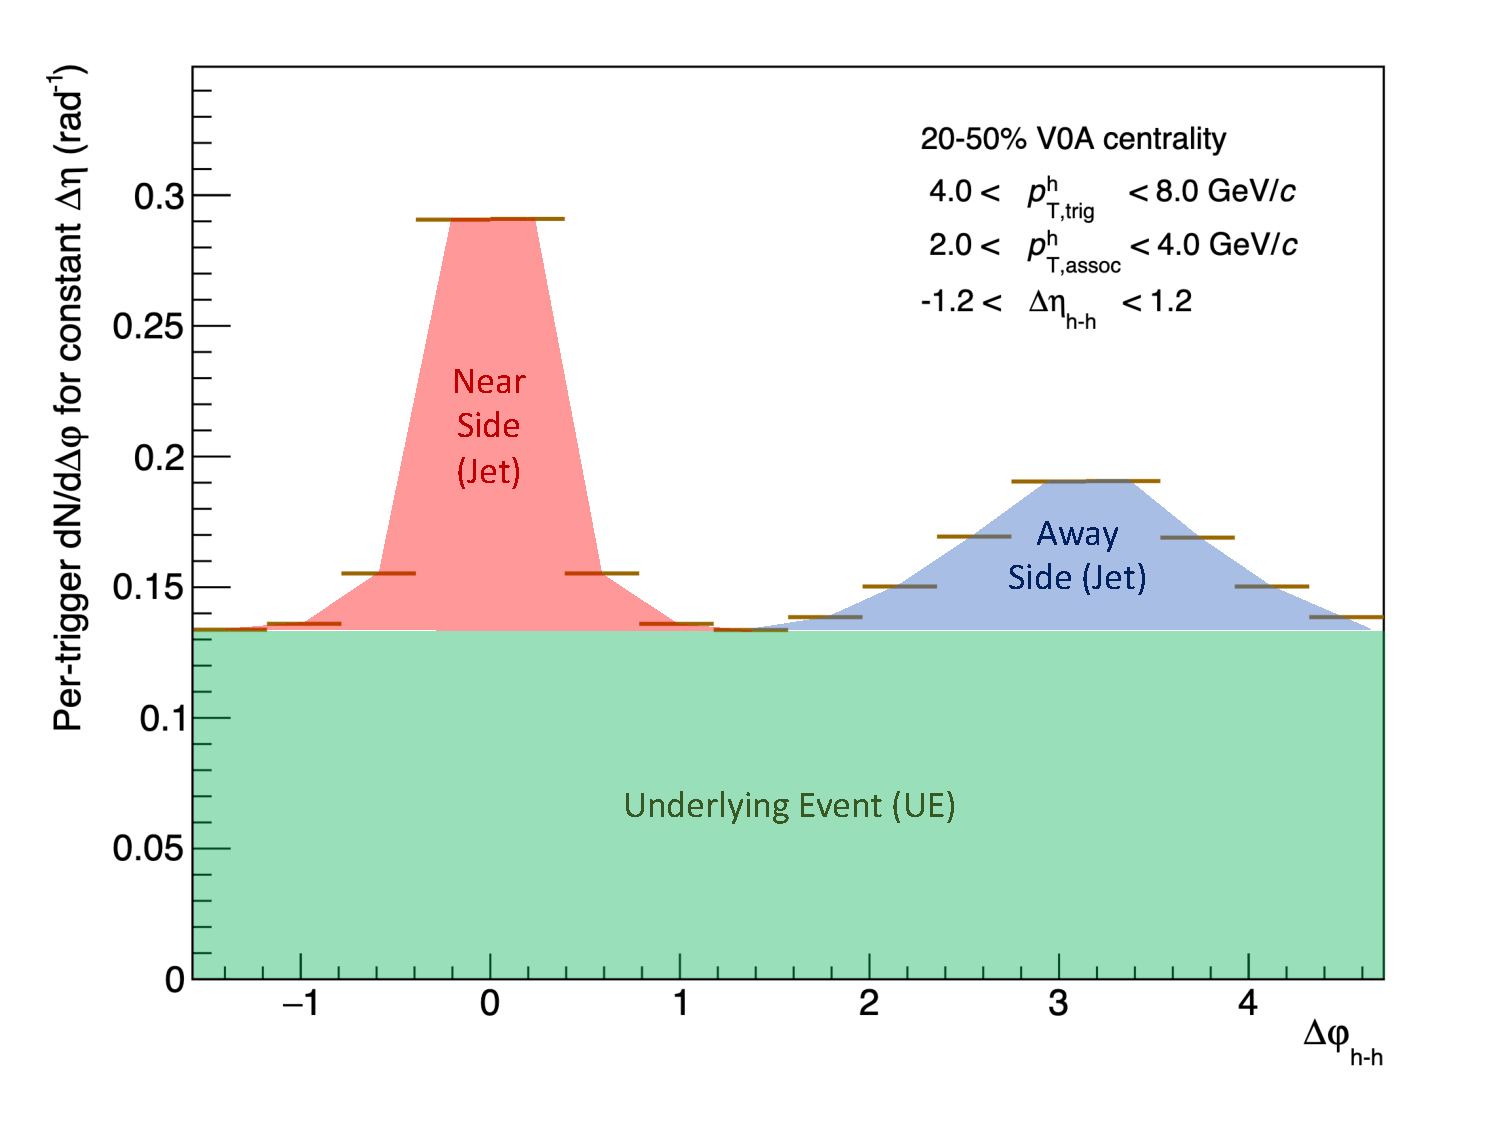
\includegraphics[width =4in]{images/dphi_regions.pdf}
\caption{Example histogram showing how the yields in the different regions of correlation space are calculated.  The green region represents the "Underlying Event", and is defined by the constant BG term of the $\Delta\varphi$ fit function.  The near- (red) and away-side (blue) Jet yields are defined as the area above the constant BG in the $-\pi/2 < \Delta\varphi < \pi/2$ and $\pi/2 < \Delta\varphi < 3\pi/2$ regions, respectively.}
\label{regions}
\end{figure}

These yields are calculated for the different multiplicity bins in both the near and away-side peaks, as well as the total yield of correlated pairs for both the $h-\phi$ and $h-h$ correlations.


\subsection{Multiplicity Dependent Ratio Measurement}

Performing the same type of fit for the $h-\phi$ and the $h-h$ correlations, we are able to measure the ratio of yields of $\frac{h-\phi}{h-h}$ correlated pairs both in the total event, as well as within the near- and away-side jets (fig.\ref{ratioplot}).

\begin{figure}[ht]
\centering
\includegraphics[width=6in]{images/approved/2019-06-04-finalratio.pdf}
\caption{Ratio of the yields of correlated $\frac{h-\phi}{h-h}$ pairs as a function of multiplicity percentile.  Near-side (away-side) yields are calculated by integrating the correlation distribution in the $-\pi/2$ to $\pi/2$ ($\pi/2$ to $3\pi/2$) and subtracting the flat background component of the $\Delta\varphi$ fit. The Underlying Event is estimated using the constant background term directly.}
\label{ratioplot}
\end{figure}

Comparing the ratio as a function of multiplicity for the different regions of correlation space, we see that the "Jet-like" yields increase as a function of multiplicity, while the "underlying event" stays relatively flat.  Since the overall yield of $\frac{h-\phi}{h-h}$ is increasing as a function of multiplicity, this suggests that the main cause of the increase in the inclusive pair ratio is due to the increase in the contribution of the "underlying event" to the total yields.  Indeed, at 50-80\% multiplicity, the total yield is comprised of ~70\% "underlying event" and 30\% "jets", while for the 0-20\% multiplicity, the total yield is comprised of ~90\% "underlying event" and 10\% jets (fig. \ref{jetratiofull}).

\begin{figure}[ht]
\centering
\includegraphics[width=4in]{images/jetratio_full.pdf}
\caption{Ratio of the yields of correlated pairs in the Jet peaks to the total number of correlated pairs for both h-h (orange) and h-$\phi$ (teal), as a function of multiplicity.  This ratio represents the percent of our correlation that is contained in within the near + away-side jets. As we move from low multiplicity to high multiplicity, we see that our jet component represents a smaller fraction of our correlation for both h-h and h-$\phi$ pairs.}
\label{jetratiofull}
\end{figure}

\section{Monte Carlo Studies}

\subsection{Correlation Method Test using Monte Carlo}

In order to test whether the full correlation measure (eq. \ref{fullCorrEq}) accurately describes the real $h-\phi$ correlation, several Monte Carlo studies were performed.  The first of these was a complete test of the correlation extraction method without detector inefficiencies.  To accomplish this test, two correlations were measured in MC dataset LHC17f2b\_FAST with the same set of high $p_T$ ($4 < p_T < \SI{8}{GeV/c}$) trigger hadrons.  The first used an associated particle taken from the MC generated $\phi$ mesons (identified via MC particle's associated PDG code), representing the real $h-\phi$ correlation. The second used the correlation method described in Section 4 to reconstruct the $h-\phi$ correlation, using the MC genereated Kaons identified via MC particle's PDG code instead of track PID cuts.

Comparing the generated vs. reconstructed correlation in $\Delta\varphi$ shows very good agreement, proving that the background subtraction method using the invariant sideband regions is sound (fig. \ref{methodtestFAST}).

\begin{figure}[ht]
\centering
\begin{subfigure}{
\includegraphics[width=3in]{images/truevsmethod.pdf}}
\end{subfigure}
\begin{subfigure}{
\includegraphics[width=3in]{images/ratio_method-true_fit.pdf}}
\end{subfigure}
\caption{Direct comparison of the generated (green) and reconstructed (red) $\Delta\varphi$ correlation, using the LHC17f2b\_FAST dataset (left). The ratio of the two distributions (right) shows that the reconstruction technique in Eq. \ref{fullCorrEq} is able to correctly capture the real $h-\phi$ correlation, with a straight line fit of the ratio giving a value of 0.99 $\pm$ 0.02}
\label{methodtestFAST}
\end{figure}

\subsection{MC Closure Test}

After the MC method test showed that the general measurement method was correctly recovering the generated $h-\phi$ correlations, a full MC closure test was performed using LHC17f2b\_FAST and LHC17f2b\_CENT datasets.  The generated correlation was taken the same way as the above method test.  For the reconstructed case, the full analysis procedure was used including tracking efficiency (Sec. \ref{corrsec}).  The reconstructed $\Delta\varphi$ distribution was then compared to the generated distribution (Fig. \ref{MCClosureFAST}).  A ratio of the two distributions fit with a straight line gives a closure of $0.98\pm 0.04$, consistent with 1.

\begin{figure}[ht]
\centering
\begin{subfigure}{
\includegraphics[width=3in]{images/truevsrecon_notrigger.pdf}}
\end{subfigure}
\begin{subfigure}{
\includegraphics[width=3in]{images/ratio_recon-true_notrigger.pdf}}
\end{subfigure}
\caption{Full MC Closure test (\textbf{left}) comparing the generated per-trigger correlation (green) with the correlation measured using the track reconstruction outlined in eq. \ref{fullCorrEq} (blue). The ratio of the two (\textbf{right}) shows good agreement with 1, within statistical fluctuations.}
\label{MCClosureFAST}
\end{figure}


\section(Resonance )
\section{Systematic Errors \& Crosschecks}


For all possible sources of systematic errors, the errors are first calculated per $\Delta\varphi$ bin in the full $\Delta\varphi$ distribution.  This is done using a ratio of all variations to the standard cut and finding the overall RMS across all $\Delta\varphi$ bin. After this is done, each variation then undergoes the full yield extraction.  The variation of the final yields is then calculated again as the RMS of all variations, giving a separate systematic error for the near-side, away-side, underlying-event, and total pair yield.  For the final $(h-\phi)/(h-h)$ pair ratios, the systematic errors from the individual $(h-\phi)$ and $(h-h$) yields are treated as uncorrelated.

\subsection()
\subsection{TOF Efficiency Crosscheck}

Since the TOF does not have uniform coverage in $\varphi$ and $\eta$, a crosscheck was necessary to ensure that the strict TOF PID signal was not influencing the final correlation measurement.  The correlation was performed separately for associated particles that fell in the angular range $0 < \varphi_{assoc} < \pi$ (with gap in TOF coverage), and in the angular range $\pi < \varphi_{assoc} < 2\pi$ (no gap in TOF coverage).  

These two correlations were then normalized to 1 to account for the different statistics and plotted against one another.  Within statistical errors, there was no difference between the correlations from one side of the detector and the other, showing that there was no effect on the final correlation shape due to the gap in TOF coverage.

\subsection{Invariant Mass Range Checks}
\label{rangeselection}
In order to test the systematic effects of the correlation method (i.e. choosing specific narrow mass regions for the "mass peak", as well as for the "side band" regions for background estimation), it is necessary to vary the width and positions of these regions and see the effect on the final correlation results.

\subsubsection{Mass Peak Region Check} 

The mass peak range can be varied by widening and narrowing the $\phi(1020)$ signal mass region considered. Since this directly changes the Signal/Background of the uncorrected correlation, this variation tests whether or not the Signal/Background of the considered region has an effect on the final correlation even after the fraction of total signal that is excluded is taken into account (i.e. the correlation is corrected by the factor $k_{\text{Signal}}$ from Eq. \ref{fullCorrEq}, which changes with the mass window used).

\begin{figure}[ht]
\centering
\begin{subfigure}{
\includegraphics[width=3in]{images/masspeakdphi.pdf}}
\end{subfigure}
\begin{subfigure}{
\includegraphics[width=3in]{images/masspeakratios.pdf}}
\end{subfigure}
\caption{$\Delta\varphi$ correlation (\textbf{left}) showing the differences between different invariant mass ranges for the $\phi(1020)$ signal region.  By looking at the ratio of these correlations to the chosen range (\SI{1.014}{GeV/c^2}$ < M_{\phi} <$ \SI{1.026}{GeV/c^2})}
\label{masspeakcheck}
\end{figure}

Within the range variation considered, we see no significant effect on the correlation function (fig. \ref{masspeakcheck}) due to the changing Signal/Background ratio. The ratio of each cut to the standard is also plotted, and found to be uniform in $\Delta\varphi$ and consistent with 1.  We also project all ratio points for each $\Delta\varphi$ bin onto a single distribution (fig. \ref{masspeakRMS}) to find an RMS value of 1.4\%, well below the statistical error of the distribution.

\begin{figure}[ht]
\centering
\includegraphics[width=3in]{images/masspeaksyst.pdf}
\caption{ }
\label{masspeakRMS}
\end{figure}


\subsubsection{Sideband Region Check}

The sideband regions of the invariant mass distribution are used for both estimating the correlation background under the mass peak, as well as for the like-sign scaling factor.  In order to make sure the choice of sideband region does not significantly change the final correlation structure, both the left and right sideband regions were varied from their standard ranges (fig. \ref{RSBcheck} \& \ref{LSBcheck}).  In both cases, variation of the sideband region shows no significant changes to the correlation distribution, with any differences well below the statistical errors of the correlation.

\begin{figure}[ht]
\centering
\begin{subfigure}{
\includegraphics[width=3in]{images/RSBrangedphi.pdf}}
\end{subfigure}
\begin{subfigure}{
\includegraphics[width=3in]{images/RSBrangeratios.pdf}}
\end{subfigure}
\caption{Plot showing the variation in final $\Delta\varphi$ correlation (\textbf{left}) from varying the right sideband invariant mass region.  This variation changes both the correlation background subtraction, as well as the likesign scaling factor. However, from the ratios of the variation to the standard range (\textbf{left}), we see this variation has no effect on the final correlation structure.}
\label{RSBcheck}
\end{figure}

\begin{figure}[ht]
\centering
\includegraphics[width=3in]{images/RSBrangesyst.pdf}
\caption{Projection of the ratio $\Delta\varphi$ points onto a single distribution shows no significant difference from the variation in right sideband region (RMS of 0.5\%)}
\label{RSBRMS}
\end{figure}

\begin{figure}[ht]
\centering
\begin{subfigure}{
\includegraphics[width=3in]{images/LSBrangedphi.pdf}}
\end{subfigure}
\begin{subfigure}{
\includegraphics[width=3in]{images/LSBrangeratio.pdf}}
\end{subfigure}
\caption{Plot showing the variation in final $\Delta\varphi$ correlation (\textbf{left}) from varying the left sideband invariant mass region.  This variation changes both the correlation background subtraction, as well as the likesign scaling factor. However, from the ratios of the variation to the standard range (\textbf{left}), we see this variation has no effect on the final correlation structure.}
\label{LSBcheck}
\end{figure}

\begin{figure}[ht]
\centering
\includegraphics[width=3in]{images/LSBrangesyst.pdf}
\caption{Projection of the ratio of $\Delta\varphi$ points from fig. \ref{LSBcheck} onto a single distribution shows no significant difference from the variation in left sideband region (RMS of 1.0\%)}
\label{LSBRMS}
\end{figure}

\subsubsection{Likesign Sideband Scaling Factor Check}

To estimate the Signal/Background ratio in the $\phi(1020)$ mass peak region, the like sign invariant mass distribution is scaled to the integral of the unlike sign sideband regions. Since this scaling factor is influenced both by the statistics of the integral (of both the like and un-like sign distributions), as well as the specific sideband mass ranges, the choice of scaling was varied between the following options:

\begin{itemize}
    \item Right Sideband only
    \item Right Sideband + Statistical Error
    \item Right Sideband - Statistical Error
    \item Left Sideband only
    \item Left Sideband + Statistical Error
    \item Left Sideband - Statistical Error
    \item Average of Left and Right Sideband
    \item Average + Statistical Error
    \item Average - Statistical Error
\end{itemize}

The "Average" case is taken to be the central value, and the ratio to the variations to the central correlation is plotted as a function of $\Delta\varphi$ (fig. \ref{scalingcheck}). Combining the ratios at each point into a single distribution (fig. \ref{scalingRMS}) gives an RMS value of ~2\%.  Since this scaling factor directly shifts the correlation function up or down, the variation cannot be ignored even with the larger statistical errors, and must be accounted for in the final systematic errors.

\begin{figure}[ht]
\centering
\begin{subfigure}{
\includegraphics[width=3in]{images/sbscalingdphi.pdf}}
\end{subfigure}
\begin{subfigure}{
\includegraphics[width=3in]{images/sbavgscalingratios.pdf}}
\end{subfigure}
\caption{Plot showing the variation in final $\Delta\varphi$ correlation (\textbf{left}) from varying the likesign scaling factor, directly changing the Signal/Background estimation.  This variation acts to shift the overall correlation up or down.}
\label{scalingcheck}
\end{figure}

\begin{figure}[ht]
\centering
\includegraphics[width=3in]{images/sbavgscalingsyst.pdf}
\caption{Projection of the ratio of all $\Delta\varphi$ points from fig. \ref{scalingcheck} onto a single distribution shows a variation due to the choice of scaling factor used (RMS of 2.0\%)}
\label{scalingRMS}
\end{figure}

\subsection{Correlation Fitting Procedure}
\label{corrfitproc}
Since there are several different methods of separating the "underlying event" from the jet peaks in the $\Delta\varphi$ correlation, a systematic check is needed to see if the final ratios are dependent on the method chosen.  The correlation consists of 16 bins in $\Delta\varphi$, and the underlying event can be estimated by looking at those bins that are farthest from the near and away jet peaks:

\begin{center}
\begin{itemize}
    \item Average of bins 1, 8, 9, 16
    \item Average of bins 1, 8, 9
    \item Average of bins 1, 2, 7, 8, 9, 16
    \item Full Correlation Fit (straight line as free parameter)
\end{itemize}
\end{center}

For the "Full Correlation Fit", the whole distribution is fit with two gaussians (the near and away-side peaks) and a straight line component.  After the full fit converges, only the straight line parameter is extracted and used as the "underyling event".

For our final systematic, we take the RMS value of the distribution of ratios given from each of the listed BG estimation procedures (fig. \ref{uesyst}). This gives us the following related systematic for the near-side, away-side, and UE:

\begin{table}[h!]
    \centering
\begin{tabular}{| c | c | c | c |}
\hline
Region & 0-20\% Error & 20-50\% Error & 50-80\% Error \\
\hline
near-side & 3.2\% & 5.8\% & 8\% \\
away-side & 8.8\% & 4.9 & 7.7\% \\
U.E. & 0.7\% & 0.7\% & 2\% \\
\hline
\end{tabular}
\caption{Systematic error in percent from the estimation method of our underlying event.}
\label{evttab}
\end{table}

\begin{figure}[ht]
\centering
\begin{subfigure}{
\includegraphics[width=3in]{images/nearside_uesyst.pdf}}
\end{subfigure}
\begin{subfigure}{
\includegraphics[width=3in]{images/awayside_uesyst.pdf}}
\end{subfigure}
\caption{Plot showing the variation in the yield ratios for the different flat background assumptions}
\label{uesyst}
\end{figure}

\subsection{PID cuts}
\label{PIDcuts}

With a relatively wide PID cut, we need to check that the inclusion of pion contamination does not effect our final correlation structure.  To do this, the TPC PID cut was varied from the standard cut of $|n\sigma_{TPC} < 3|$ to 2.8, 2.6, 2.4, 2.2 and 2.0.

\subsection{Affect of v2 Assumption on Ratios}

Since the near and away-side peak (and underlying event) yields are calculated based on the assumption of a flat background underneath the jets, an additional check is needed to see if the inclusion of a v2 term changes the final $(h-\phi)/(h-h)$ ratios.  Since a published value for $\phi$ $v_2$ in p-Pb was not available, we chose to use the published values for inclusive charged hadrons to estimate a systematic error.  Using the published ALICE values (https://doi.org/10.1016/j.physletb.2013.08.024) gives us a $v_2$ in the 0-20\% bin of 0.15, while the 20-50\% and 50-80\% values are taken as 85\% and 50\% of the high multiplicity value, respectively.

By computing the pair yields using the non-zero $v_2$ values, we can compare the effect on the (h-$\phi$)/(h-h) ratio measurement to our flat background assumption.  Since the (h-h) and (h-$\phi$) correlations are treated with the same charge particle $v_2$, the overall effect on the ratio is a slight decrease in the jet yields at high multiplicity.  On the other hand, since the non-jet component is so dominant within our correlation momentum ranges, the non-zero $v_2$ does not have a visible effect on the Underlying Event ratio.


\clearpage
\appendix
\section{Second Momentum Bin Measurement}

In order to further study the $\phi(1020)$ production in jets vs. the underlying event, we can also split the associated momentum bin into a high and low $p_{\text{T}}$ component.  This allows us to look at the same measurement in a more jet-dominated regime (higher momentum) and in a more underlying-event dominated regime (lower momentum). For this purpose, we chose the associated momentum bins of $1.5 < p^{\phi}_{\text{T}} < \SI{2.5}{GeV/c}$ for the lower bin, and $2.5 < p^{\phi}_{\text{T}} < \SI{4.0}{GeV/c}$ for the higher momentum bin.  The correlation analysis is performed for these two separate momentum bins exactly as laid out in Section 4, and is done for both h-$\phi$ and h-h correlated pairs.

\begin{figure}[ht]
\centering
\begin{subfigure}{
\includegraphics[width=5in]{images/addendum/dphi_hphi_25-40.pdf}}
\end{subfigure}
\begin{subfigure}{
\includegraphics[width=5in]{images/addendum/dphi_hphi_15-25.pdf}}
\end{subfigure}
\caption{h-$\phi$ correlations for both the higher momentum (top) and lower momentum (bottom) regimes, after the underlying event has been subtracted.  Jet peaks are structurally similar between the two momentum bins, within the increased errors due to decreased statistics.}
\label{split_momentum_corr}
\end{figure}

By comparing the ratio of $(h-\phi)/(h-h)$ pairs in these two different momentum regimes (fig. \ref{high_momentum_ratio} \& \ref{low_momentum_ratio}), we can see that the general trends of an enhanced $\phi$ production in the Underlying Event, and the increase in $\phi/h$ production as a function of multiplicity, both hold true.  This suggests that these general trends are not influenced by being measured in a more jet-production dominated regime (high momentum) vs. an underlying-event production dominated regime (low momentum).

\begin{figure}[ht]
\centering
\includegraphics[width=5in]{images/addendum/ratio_25-40.pdf}
\caption{}
\label{high_momentum_ratio}
\end{figure}

\begin{figure}[ht]
\centering
\includegraphics[width=5in]{images/addendum/ratio_15-25.pdf}
\caption{}
\label{low_momentum_ratio}
\end{figure}

We also note that the low momentum regime shows a smaller separation between the jet-like production and the underlying event production across all multiplicities. In addition, there is a steeper increase in the ratio within the away-side jet as a function of multiplicity, hinting that jet-medium interactions in the low momentum region may be causing the away-side $h-\phi/h-h$ ratio to approach the underlying event ratio at high multiplicity (fig. \ref{low_momentum_ratio}).

In looking at the underlying event production, the lower momentum $h-\phi/h-h$ ratio shows a little increase across multiplicity, while for the higher momentum region, we see a marked enhancement.  In both momentum regions, the Total ratio's increase as a function of multiplicity is driven in part by the shrinking jet contribution as multiplicity increases.

\section{Resonance Technique for $\Lambda$ Reconstruction}
\label{resonance_technique}

While using the V0 finder to reconstruct $\Lambda$ baryons is the most common method, it is possible that the V0 finder alogrithm introduces some topological biases in the $\Lambda$ reconstruction, even when no further topological cuts are being applied to the V0 or its corresponding daughters. Because of this, we also investigate another method for reconstructing $\Lambda$ baryons whereby all proton and pion pairs from the global AOD track list that pass the daughter cuts (Section \ref{daughtercuts}) within an event are combined to reconstruct the $\Lambda$s. This method is referred to as the \it{resonance technique}, as it is the technique used to reconstruct short-lived particles that could otherwise not be reconstructed using the V0 finder.

\subsection{Combinatorial Background Estimation}

As $\Lambda$ baryons reconstructed using the resonance technique will have a large combinatorial background, the final correlation will contain $h-(p\pi)$ pairs that need to be removed. In order to remove this background, we need both an estimate of the correlation shape of the $h-(p\pi)$ pairs, as well as an estimate of the Signal/Background in the $\Lambda$ mass peak region.

 The background shape of the $\Lambda$ invariant mass distribution can be estimated using one of the two following techniques:

 \begin{itemize}
	\item \textbf{Like-sign $p\pi$ pairs} - Reconstruct the invariant mass of like-sign $p\pi$ pairs, and scale the like-sign $p\pi$ distribution to the un-like sign $p\pi$ distribution in a region outside of the $\Lambda$ signal region.
	\item \textbf{Rotated $p\pi$ pairs} - Reconstruct the invariant mass of unlike-sign $p\pi$ pairs, but rotate either the pion or proton around the z-axis by $\pi$ radians, and scale the rotated $p\pi$ distribution to the un-like sign $p\pi$ distribution in a region outside of the $\Lambda$ signal region.
 \end{itemize}

To determine which of these techniques is more effective, we compare the background shape of the $\Lambda$ invariant mass distribution for both techniques in MonteCarlo where we have direct access to the background shape. The like-sign and rotated $p\pi$ pairs are shown along with the extracted signal comparsion in Figure \ref{background_approx_MC}. The like-sign $p\pi$ pairs match the background shape of the $\Lambda$ invariant mass distribution more closely than the rotated $p\pi$ pairs, so we use the like-sign $p\pi$ pairs to estimate the combinatorial background in the $\Lambda$ invariant mass distribution in data.

\begin{figure}[ht]
	\centering
	\begin{subfigure}{
	\includegraphics[width=3in]{figures/background_approx_MC.pdf}}
	\end{subfigure}
	\begin{subfigure}{
	\includegraphics[width=3in]{figures/background_subtracted_signal_MC.pdf}}
	\end{subfigure}
	\caption{Left: Invariant Mass distribution for unlike-sign $p\pi$ pairs (black) in our MonteCarlo sample.  The like-sign $p\pi$ pair mass distribution (purple) and unlike-sign rotated $p\pi$ distributions are scaled to match the unlike-sign distribution within the invariant mass region. The true combinatorial background (red) matches most closesly with the like-sign pairs. Right: The actual $\Lambda$ signal (magenta) compared with the result of subracting the like-sign from the total unlike-sign $p\pi$ distribution (green). The two distributions show good agreement.}
	\label{background_approx_MC}
	\end{figure}
	
	The region outside of the $\Lambda$ signal region used for scaling the background estimates is called the Right SideBand region, or RSB. The choice of RSB has a large systematical effect on the background approximation as neither the like-sign nor rotated $p\pi$ pairs match the background shape throughout the entirety of the distribution. The RSBs were chosen for each multiplicity bin to minimize the difference in shape between the extracted signal in data (total - like-sign BG) and the resonance-technique reconstructed signal shape in MonteCarlo, generated from all $p\pi$ pairs which guaranteed came from a $\Lambda$. The raw unlike-sign $p\pi$ distribution for the 0-20\% Multiplicity Percentile is shown in Figure \ref{res_invariant_mass_0_20}, and the extracted signal and comparison with MonteCarlo is shown in Figure \ref{res_invariant_mass_signal_0_20}.
	
	
	\begin{figure}[ht]
	\centering
	\begin{subfigure}{
	\includegraphics[width=3in]{figures/lambda_mass_0_20_resonance_with_ls_with_rsb.pdf}}
	\end{subfigure}
	\begin{subfigure}{
	\includegraphics[width=3in]{figures/lambda_mass_0_20_resonance_signal_comp.pdf}}
	\end{subfigure}
	\caption{Left: Invariant Mass distribution for unlike-sign $p\pi$ pairs (black) along with the like-sign $p\pi$ background (purple) and the RSB region (red) in the 0-20\% multiplicity bin. Right: The extracted signal (green) compared with the resonance-technique reconstructed signal shape in MonteCarlo (magenta). The RSB was chosen such that these shapes are similar. }
	\label{res_invariant_mass_0_20}
	\end{figure}


\subsection{Invariant Mass Regions}

The signal shape and background from $\Lambda$s reconstructed using the resonance technique is vastly different than those reconstructed using the V0 finder, thus it is necessarry to define new invariant mass regions such that the signal can be properly extracted:

\begin{itemize}
	\item \makebox[7.5cm][l]{unlike-sign $p\pi$ in $\Lambda$ mass region:}  \SI{1.014}{GeV/c^2}$< M_{p\pi} < $\SI{1.026}{GeV/c^2}
	\item \makebox[7.5cm][l]{like-sign $p\pi$ in $\Lambda$ mass region:}  \SI{1.014}{GeV/c^2}$< M_{p\pi} < $\SI{1.026}{GeV/c^2}
	\item  \makebox[7.5cm][l]{unlike-sign $p\pi$ in 0-20\% multiplicity bin RSB:}  \SI{0.995}{GeV/c^2}$< M_{p\pi} < $\SI{1.005}{GeV/c^2}
	\item  \makebox[7.5cm][l]{unlike-sign $p\pi$ in 20-50\% multiplicity bin RSB:}  \SI{0.995}{GeV/c^2}$< M_{p\pi} < $\SI{1.005}{GeV/c^2}
	\item  \makebox[7.5cm][l]{unlike-sign $p\pi$ in 50-80\% multiplicity bin RSB:}  \SI{0.995}{GeV/c^2}$< M_{p\pi} < $\SI{1.005}{GeV/c^2}
\end{itemize}

The signal regions were chosen to maximize significance and were not multiplicty dependent, whereas the RSB regions were chosen to minimize the difference in shape between the extracted signal in data (total - like-sign BG) and the resonance-technique reconstructed signal shape in MonteCarlo, generated from all $p\pi$ pairs which guaranteed came from a $\Lambda$, as was demonstrated in Figure \ref{res_invariant_mass_0_20}. This process was repeated for each multiplicity bin resulting in slight fluctuations of the RSB with respect to multiplicity.

For the resonance technique, the combinatorial background contribution to the correlation was removed using the like-sign $p\pi$ distribution scaled to the RSB for each mulitiplicty bin, a procedure described with more detail in Section \ref{resonance_technique_bg_subtraction}.


 


\section{Jet vs. Total Production comparison}

To get a quantitative look at the differences between low multiplicity events (more jet) and high multiplicity events (more underlying event) and the effect this has on the correlation ratios, we can measure the ratio of Jet pairs over Total pairs (i.e. the fraction of correlated pairs that are in a jet) (fig. \ref{jetvstot}).

\begin{figure}[ht]
\centering
\begin{subfigure}{
\includegraphics[width=3in]{images/addendum/jet2totratio_lowpt.pdf}}
\end{subfigure}
\begin{subfigure}{
\includegraphics[width=3in]{images/addendum/jet2totratio_highpt.pdf}}
\end{subfigure}
\caption{Fraction of Jet Produced correlated pairs as a function of multiplicity for low momentum (left) and high momentum (right) regions.  In both momentum regions, the Jet fraction of h-h pairs decreases significantly as a function of multiplicity.  For h-$\phi$ pairs, however, the overall fraction coming from jets only slightly decreases as multiplicity increases.}
\label{jetvstot}
\end{figure}

From this measurement, there is a clear difference in behavior of jet production of associated $\phi$ mesons vs. associated inclusive hadrons as multiplicity increases.  The fraction of jet-produced hadrons shows a sharp decrease as a function of multiplicity, while the fraction of jet-produced $\phi$ mesons is significantly lower and flatter as a function of multiplicity. This shows that the balance of production methods of $\phi$ mesons are mostly independent of multiplicity, while the production methods of hadrons significantly shifts from jet production towards underlying event production as multiplicity increases.

\section{Investigating Radial Flow Effects}

The two momentum bins chosen show that there is a relatively narrow momentum range (approx. $2 < p_{\text{T}} < \SI{4}{GeV/c}$ that contains sufficient jet production as well as sufficient production in the underlying event to give a statistically meaningful comparison.  However, since this ratio is performed in a narrow range, an additional check was performed to look for the effect of radial flow pushing particles into this momentum range as multiplicity increases.

For this purpose, a simple Boltzmann model was chosen to reflect the effect of the radial flow on the spectra of the different particle species:

\begin{align}
    B(p_{\text{T}}) = \frac{C}{T(m+T)}p_{\text{T}}\exp{-(m_{\text{T}}-m)/T}
\end{align}

where $m$ is the particle's mass, $m_{\text{T}}$ is the transverse mass, $C$ is a scaling parameter, and $T$ is the free temperature parameter.

For each particle species, $T$ was found such that the $\langle p_{\text{T}}\rangle$ for the Boltzmann distribution for a given multiplicity matched with the measured $\langle p_{\text{T}}\rangle$ previously reported by ALICE (fig. \ref{mean_pt}).

\begin{figure}[ht]
\centering
\begin{subfigure}{
\includegraphics[width=2.8in]{images/addendum/boltz/boltz_temp.png}
}
\end{subfigure}
\begin{subfigure}{
\includegraphics[width=3in]{images/addendum/boltz/pub_meanpt.png}
}
\end{subfigure}
\caption{Temperature of the Boltzmann model for different particle species and multiplicities (left) to match the Boltzmann spectra $\langle p_{T}\rangle$ to the published ALICE values (right).}
\label{mean_pt}
\end{figure}

After fitting the temperatures of the Boltzmann spectra to the measured $\langle p_{\text{T}} \rangle$, the spectra were compared between low and high multiplicity regions to see the effect of the increased temperature on production in our chosen momentum region (fig. \ref{boltzspectra}).  This shows that the lower mass particles have a larger shift into our momentum region than the $\phi$ meson, due to the fact that the $\phi$ has a much higher $\langle p_{\text{T}} \rangle$ than the other particle species.

\begin{figure}[ht]
\centering
\begin{subfigure}{
\includegraphics[width=2.8in]{images/addendum/boltz/boltz_phispectra.png}
}
\end{subfigure}
\begin{subfigure}{
\includegraphics[width=3in]{images/addendum/boltz/boltz_pispectra.png}
}
\end{subfigure}
\caption{Boltzmann model spectra comparison between a low and high multiplicity bin for the $\phi$ (left) and pion (right). While both particles are shifted to high momentum at high multiplicity, the pion sees a much larger increase in the marked $2 < p_{\text{T}} < \SI{4}{GeV/c}$ region}
\label{boltzspectra}
\end{figure}

From these normalized model Boltzmann Spectra, a ratio is constructed in the $2 < p_{\text{T}} < \SI{4}{GeV/c}$ region to see the effect this simplified radial flow model would have on the final ratio results (fig. \ref{boltzratio}).  Since the $\phi$ has a much larger $\langle p_{\text{T}} \rangle$, and therefore experiences less of a shift into this region, the overal effect is actually a decrease in the $\phi/h$ ratio vs multiplicity within this momentum region. As this is the opposite of what we see in the measured $\phi/h$ ratio, we conclude this effect is not confounded our measurement of strangeness enhancement.

\begin{figure}[ht]
\centering
\includegraphics[width=4in]{images/addendum/boltz/boltzratio.png}
\caption{Normalized ratio of $\phi$ to stable hadrons vs. multiplicity based on the simplified Boltzmann model fit from measured $\langle p_{\text{T}} \rangle$ in the region $2 < p_{\text{T}} < \SI{4}{GeV/c}$.  From the model results, the effect of increased $\langle p_{\text{T}} \rangle$ would actually decrease the $\phi/h$ ratio due to the much higher $\langle p_{\text{T}} \rangle$ of the $\phi$ compared to the other hadrons.}
\label{boltzratio}
\end{figure}

\section{Single Trigger Selection and Results}

Since the correlation measurement gives per-trigger yields of associated pairs , rather than the associated particles directly, it is possible that event-by-event fluctuations in the number of trigger and associated particles can lead to a small difference between the ratio of associated pairs and associated particles. While the number of events with multiple trigger particles in the defined momentum range $4 < p_{\text{T}} < \SI{8}{GeV/c}$ is only $~12\%$ (and therefore the possibility of discrepancy is limited), an additional crosscheck was performed to look for any effect this had on the final measurement.

For this crosscheck, only a single trigger particle was chosen from each event for the correlation (fig. \ref{singletrigcorr}).  In events with multiple triggers in the $4 < p_{\text{T}} < \SI{8}{GeV/c}$, only the highest momentum trigger was kept.  In this way, the correlation measurement is changed from a per-trigger yield to a per-triggered-event yield, with the presence of at least one $4 < p_{\text{T}} < \SI{8}{GeV/c}$ hadron being the trigger condition.

\begin{figure}[!htb]
\centering
\includegraphics[width=6in]{images/addendum/singletrig_dphi.png}
\caption{Comparison between the standard per-trigger correlation (solid markers) and the highest-trigger correlation (open markers) for the 20-50\% multiplicity bin.}
\label{singletrigcorr}
\end{figure}

Dividing the per-trigger measurement by the single-trigger measurement,  effects on the final $\Delta\varphi$ correlations is seen to be a flat scale factor across multiplicity. This scale factor for the (h-h) correlation is found to be ~1.2, while the (h-$\phi$) correlation is essentially unchanged (fig. \ref{singletrigratio}).  The slight difference seen in the structure of the (h-h) correlation is caused by the hardening of the trigger spectra (since choosing the highest trigger will skew the trigger momentum).

\begin{figure}[!htb]
\centering
\includegraphics[width=6in]{images/addendum/singletrig_ratio.png}
\caption{Ratio of the standard per-trigger correlation to the single-trigger correlation. The effect of choosing a single high trigger is a constant scaling across all multiplicities.  Since most events that have a $\phi$ meson only have a single $\phi$ meson, the change in trigger scaling has a negligible effect on the $h-\phi$ correlation.}
\label{singletrigratio}
\end{figure}

Since the single trigger analysis acts as a flat scale factor on our original correlation, the effect on our measurement would only be a change of scale on the final $\phi/h$ ratio.  This shows the validity of our method of using standard per-trigger correlations to accurately capture the behavior of the $\phi/h$ ratio in different production regimes, while also demonstrating the care that needs to be taken when directly comparing this measurement to inclusive $\phi/h$ yield measurements. 

\clearpage
\section {Additional Plots}

\subsection{Approved Plots}

\begin{figure}[!htb]
\centering
\includegraphics[width=4in]{images/approved/2019-06-05-invmass_raw.pdf}
\caption{}
\label{}
\end{figure}

\begin{figure}[!htb]
\centering
\includegraphics[width=4in]{images/approved/2019-06-05-invmass_corr.pdf}
\caption{}
\label{}
\end{figure}

\begin{figure}[!htb]
\centering
\includegraphics[width=4in]{images/approved/2019-06-04-dphi_bgcompare.pdf}
\caption{}
\label{}
\end{figure}

\begin{figure}[!htb]
\centering
\includegraphics[width=4in]{images/approved/2019-06-05-dphi_SBcompare.pdf}
\caption{}
\label{}
\end{figure}

\begin{figure}[!htb]
\centering
\begin{subfigure}{
\includegraphics[width=6in]{images/approved/2019-06-05-dphi_hhall.pdf}}
\end{subfigure}
\begin{subfigure}{
\includegraphics[width=6in]{images/approved/2019-06-05-dphi_hphiall.pdf}
}
\end{subfigure}
\caption{}
\label{}
\end{figure}

\clearpage
\subsection{Misc. Plots}

\begin{figure}[!htb]
\centering
\begin{subfigure}{
\includegraphics[width=3in]{images/addendum/hh_50_80_fullbg.pdf}
}
\end{subfigure}
\begin{subfigure}{
\includegraphics[width=3in]{images/addendum/hphi_50_80_fullbg.pdf}
}
\end{subfigure}
\caption{}
\label{}
\end{figure}

\begin{figure}[!htb]
\centering
\begin{subfigure}{
\includegraphics[width=3in]{images/addendum/hh_20_50_fullbg.pdf}
}
\end{subfigure}
\begin{subfigure}{
\includegraphics[width=3in]{images/addendum/hphi_20_50_fullbg.pdf}
}
\end{subfigure}
\caption{}
\label{}
\end{figure}

\begin{figure}[!htb]
\centering
\begin{subfigure}{
\includegraphics[width=3in]{images/addendum/hh_0_20_fullbg.pdf}
}
\end{subfigure}
\begin{subfigure}{
\includegraphics[width=3in]{images/addendum/hphi_0_20_fullbg.pdf}
}
\end{subfigure}
\caption{}
\label{}
\end{figure}
\end{document}